\documentclass{article}\usepackage[]{graphicx}\usepackage[]{color}
%% maxwidth is the original width if it is less than linewidth
%% otherwise use linewidth (to make sure the graphics do not exceed the margin)
\makeatletter
\def\maxwidth{ %
  \ifdim\Gin@nat@width>\linewidth
    \linewidth
  \else
    \Gin@nat@width
  \fi
}
\makeatother

\definecolor{fgcolor}{rgb}{0.345, 0.345, 0.345}
\newcommand{\hlnum}[1]{\textcolor[rgb]{0.686,0.059,0.569}{#1}}%
\newcommand{\hlstr}[1]{\textcolor[rgb]{0.192,0.494,0.8}{#1}}%
\newcommand{\hlcom}[1]{\textcolor[rgb]{0.678,0.584,0.686}{\textit{#1}}}%
\newcommand{\hlopt}[1]{\textcolor[rgb]{0,0,0}{#1}}%
\newcommand{\hlstd}[1]{\textcolor[rgb]{0.345,0.345,0.345}{#1}}%
\newcommand{\hlkwa}[1]{\textcolor[rgb]{0.161,0.373,0.58}{\textbf{#1}}}%
\newcommand{\hlkwb}[1]{\textcolor[rgb]{0.69,0.353,0.396}{#1}}%
\newcommand{\hlkwc}[1]{\textcolor[rgb]{0.333,0.667,0.333}{#1}}%
\newcommand{\hlkwd}[1]{\textcolor[rgb]{0.737,0.353,0.396}{\textbf{#1}}}%

\usepackage{framed}
\makeatletter
\newenvironment{kframe}{%
 \def\at@end@of@kframe{}%
 \ifinner\ifhmode%
  \def\at@end@of@kframe{\end{minipage}}%
  \begin{minipage}{\columnwidth}%
 \fi\fi%
 \def\FrameCommand##1{\hskip\@totalleftmargin \hskip-\fboxsep
 \colorbox{shadecolor}{##1}\hskip-\fboxsep
     % There is no \\@totalrightmargin, so:
     \hskip-\linewidth \hskip-\@totalleftmargin \hskip\columnwidth}%
 \MakeFramed {\advance\hsize-\width
   \@totalleftmargin\z@ \linewidth\hsize
   \@setminipage}}%
 {\par\unskip\endMakeFramed%
 \at@end@of@kframe}
\makeatother

\definecolor{shadecolor}{rgb}{.97, .97, .97}
\definecolor{messagecolor}{rgb}{0, 0, 0}
\definecolor{warningcolor}{rgb}{1, 0, 1}
\definecolor{errorcolor}{rgb}{1, 0, 0}
\newenvironment{knitrout}{}{} % an empty environment to be redefined in TeX

\usepackage{alltt}
\usepackage{geometry}
\usepackage{amsmath}
\usepackage{lscape}
\geometry{verbose,tmargin=2.5cm,bmargin=2.5cm,lmargin=2.5cm,rmargin=2.5cm}
\IfFileExists{upquote.sty}{\usepackage{upquote}}{}
\begin{document}



\title{NSWPCN Predictor Training}
\maketitle

%%%%%%%%%%%%%%%%%%%%%%%%%%%%%%%%%%%%%%%%%%%%%%%%%%%%%%%%%%%%%%%%%%%%%%
% LIBRARIES
%%%%%%%%%%%%%%%%%%%%%%%%%%%%%%%%%%%%%%%%%%%%%%%%%%%%%%%%%%%%%%%%%%%%%%
\section{Preparation}
\begin{knitrout}
\definecolor{shadecolor}{rgb}{0.969, 0.969, 0.969}\color{fgcolor}\begin{kframe}
\begin{alltt}
\hlkwd{library}\hlstd{(survival)}
\end{alltt}


{\ttfamily\noindent\itshape\color{messagecolor}{\#\# Loading required package: splines}}\begin{alltt}
\hlkwd{library}\hlstd{(glmulti)}
\end{alltt}


{\ttfamily\noindent\itshape\color{messagecolor}{\#\# Loading required package: rJava}}\begin{alltt}
\hlkwd{library}\hlstd{(flexsurv)}
\hlkwd{library}\hlstd{(randomForestSRC)}
\end{alltt}


{\ttfamily\noindent\itshape\color{messagecolor}{\#\# Loading required package: parallel\\\#\# \\\#\#\ \ randomForestSRC 1.5.5 \\\#\#\ \ \\\#\#\ \ Type rfsrc.news() to see new features, changes, and bug fixes. \\\#\# }}\begin{alltt}
\hlkwd{library}\hlstd{(reshape2)}
\hlkwd{library}\hlstd{(plyr)}
\hlkwd{library}\hlstd{(ggplot2)}

\hlkwd{library}\hlstd{(MASS)}
\hlkwd{library}\hlstd{(boot)}
\end{alltt}


{\ttfamily\noindent\itshape\color{messagecolor}{\#\# \\\#\# Attaching package: 'boot'\\\#\# \\\#\# The following object is masked from 'package:survival':\\\#\# \\\#\#\ \ \ \  aml}}\begin{alltt}
\hlkwd{library}\hlstd{(timeROC)}
\end{alltt}


{\ttfamily\noindent\itshape\color{messagecolor}{\#\# Loading required package: pec\\\#\# Loading required package: mvtnorm\\\#\# Loading required package: timereg}}\begin{alltt}
\hlkwd{source}\hlstd{(}\hlstr{"stdca.R"}\hlstd{)}

\hlkwd{load}\hlstd{(}\hlstr{"03_NSWPCN_subset.rda"}\hlstd{)}
\end{alltt}
\end{kframe}
\end{knitrout}


%%%%%%%%%%%%%%%%%%%%%%%%%%%%%%%%%%%%%%%%%%%%%%%%%%%%%%%%%%%%%%%%%%%%%%
% DATA SELECTION
%%%%%%%%%%%%%%%%%%%%%%%%%%%%%%%%%%%%%%%%%%%%%%%%%%%%%%%%%%%%%%%%%%%%%%
\section{Cohort selection and transformation}
\begin{knitrout}
\definecolor{shadecolor}{rgb}{0.969, 0.969, 0.969}\color{fgcolor}\begin{kframe}
\begin{alltt}
\hlstd{x} \hlkwb{=} \hlstd{data[,}\hlkwd{c}\hlstd{(}\hlstr{"Patient.Sex"}\hlstd{,} \hlstr{"History.Diagnosis.AgeAt.Cent"}\hlstd{,} \hlstr{"Path.LocationBody"}\hlstd{,} \hlstr{"Path.Size.Cent"}\hlstd{,} \hlstr{"Path.Ca199.Preop"}\hlstd{,} \hlstr{"Molec.S100A2.DCThresh"}\hlstd{,} \hlstr{"Molec.S100A4.DCThresh"}\hlstd{)]}
\hlkwd{colnames}\hlstd{(x)} \hlkwb{=} \hlkwd{c}\hlstd{(}\hlstr{"SexM"}\hlstd{,} \hlstr{"AgeCent"}\hlstd{,} \hlstr{"LocBody"}\hlstd{,} \hlstr{"SizeCent"}\hlstd{,} \hlstr{"Ca199"}\hlstd{,} \hlstr{"A2"}\hlstd{,} \hlstr{"A4"}\hlstd{)}
\hlstd{x}\hlopt{$}\hlstd{SexM} \hlkwb{=} \hlstd{x}\hlopt{$}\hlstd{Sex} \hlopt{==} \hlstr{"M"}
\hlstd{x}\hlopt{$}\hlstd{Ca199} \hlkwb{=} \hlstd{x}\hlopt{$}\hlstd{Ca199} \hlopt{>} \hlnum{100}

\hlstd{y} \hlkwb{=} \hlkwd{Surv}\hlstd{(}\hlkwd{as.numeric}\hlstd{(data}\hlopt{$}\hlstd{History.Death.Date} \hlopt{-} \hlstd{data}\hlopt{$}\hlstd{History.Diagnosis.Date), data}\hlopt{$}\hlstd{History.DSDeath.Event)}
\hlcom{# Note no surgery dates, though for almost all pts there were only a few days difference.}

\hlstd{temp} \hlkwb{=} \hlnum{NA}
\hlstd{temp} \hlkwb{=} \hlkwd{ls}\hlstd{()}
\hlkwd{rm}\hlstd{(}\hlkwc{list} \hlstd{= temp[}\hlopt{!}\hlstd{(temp} \hlopt \hlkwd{c}\hlstd{(}\hlstr{"x"}\hlstd{,} \hlstr{"y"}\hlstd{))])}

\hlstd{sel} \hlkwb{=} \hlopt{!}\hlkwd{is.na}\hlstd{(y[,}\hlnum{1}\hlstd{])} \hlopt{& !}\hlkwd{is.na}\hlstd{(y[,}\hlnum{2}\hlstd{])} \hlopt{& !}\hlkwd{is.na}\hlstd{(x}\hlopt{$}\hlstd{A2)} \hlopt{& !}\hlkwd{is.na}\hlstd{(x}\hlopt{$}\hlstd{A4)} \hlopt{& !}\hlkwd{is.na}\hlstd{(x}\hlopt{$}\hlstd{LocBody)}
\hlstd{x} \hlkwb{=} \hlstd{x[sel,]}
\hlstd{y} \hlkwb{=} \hlstd{y[sel,]}
\hlkwd{rm}\hlstd{(sel)}

\hlcom{# Remove CA-19-9 measurements as they're mostly missing}
\hlstd{x} \hlkwb{=} \hlstd{x[,}\hlkwd{colnames}\hlstd{(x)} \hlopt{!=} \hlstr{"Ca199"}\hlstd{]}

\hlstd{data} \hlkwb{=} \hlkwd{as.data.frame}\hlstd{(}\hlkwd{cbind}\hlstd{(}\hlkwc{Time} \hlstd{= y[,}\hlnum{1}\hlstd{],} \hlkwc{DSD} \hlstd{= y[,}\hlnum{2}\hlstd{], x))}
\hlkwd{rm}\hlstd{(x, y)}
\hlstd{data}\hlopt{$}\hlstd{DSD} \hlkwb{=} \hlstd{data}\hlopt{$}\hlstd{DSD} \hlopt{==} \hlnum{1}
\end{alltt}
\end{kframe}
\end{knitrout}


%%%%%%%%%%%%%%%%%%%%%%%%%%%%%%%%%%%%%%%%%%%%%%%%%%%%%%%%%%%%%%%%%%%%%%
% DATA SPLITTING
%%%%%%%%%%%%%%%%%%%%%%%%%%%%%%%%%%%%%%%%%%%%%%%%%%%%%%%%%%%%%%%%%%%%%%
\section{Data splitting}
There's going to be an awful lot of model manipulation and black magic going on.  Create a holdout validation set for final model comparison and selection.
\begin{knitrout}
\definecolor{shadecolor}{rgb}{0.969, 0.969, 0.969}\color{fgcolor}\begin{kframe}
\begin{alltt}
\hlkwd{set.seed}\hlstd{(}\hlnum{20150110}\hlstd{)}
\hlstd{sel.val} \hlkwb{=} \hlkwd{sample.int}\hlstd{(}\hlkwd{nrow}\hlstd{(data),} \hlkwd{floor}\hlstd{(}\hlkwd{nrow}\hlstd{(data)}\hlopt{/}\hlnum{4}\hlstd{))}
\hlstd{sel.val} \hlkwb{=} \hlnum{1}\hlopt{:}\hlkwd{nrow}\hlstd{(data)} \hlopt \hlstd{sel.val}
\hlkwd{mean}\hlstd{(sel.val)}
\end{alltt}
\begin{verbatim}
## [1] 0.25
\end{verbatim}
\begin{alltt}
\hlstd{data.val} \hlkwb{=} \hlstd{data[sel.val,,}\hlkwc{drop} \hlstd{=} \hlnum{FALSE}\hlstd{]}
\hlstd{data} \hlkwb{=} \hlstd{data[}\hlopt{!}\hlstd{sel.val,,}\hlkwc{drop} \hlstd{=} \hlnum{FALSE}\hlstd{]}
\end{alltt}
\end{kframe}
\end{knitrout}


%%%%%%%%%%%%%%%%%%%%%%%%%%%%%%%%%%%%%%%%%%%%%%%%%%%%%%%%%%%%%%%%%%%%%%
% MODEL SPECIFICATION
%%%%%%%%%%%%%%%%%%%%%%%%%%%%%%%%%%%%%%%%%%%%%%%%%%%%%%%%%%%%%%%%%%%%%%
\section{EDA}
Use the CPH model as a convenient framework for EDA.
\subsection{Functional form}
Investigate functional form with martingale residuals.
\begin{knitrout}
\definecolor{shadecolor}{rgb}{0.969, 0.969, 0.969}\color{fgcolor}\begin{kframe}
\begin{alltt}
\hlstd{fit.cph.NoAge} \hlkwb{=} \hlkwd{coxph}\hlstd{(}\hlkwd{Surv}\hlstd{(Time, DSD)} \hlopt{~} \hlstd{SexM} \hlopt{+} \hlstd{LocBody} \hlopt{+} \hlstd{SizeCent} \hlopt{+} \hlstd{A2} \hlopt{+} \hlstd{A4,} \hlkwc{data} \hlstd{= data)}
\hlkwd{scatter.smooth}\hlstd{(data}\hlopt{$}\hlstd{AgeCent,} \hlkwd{resid}\hlstd{(fit.cph.NoAge,} \hlkwc{type} \hlstd{=} \hlstr{"martingale"}\hlstd{),} \hlkwc{xlab} \hlstd{=} \hlstr{""}\hlstd{,} \hlkwc{ylab} \hlstd{=} \hlstr{"Martingale residual"}\hlstd{)}
\end{alltt}
\end{kframe}

{\centering 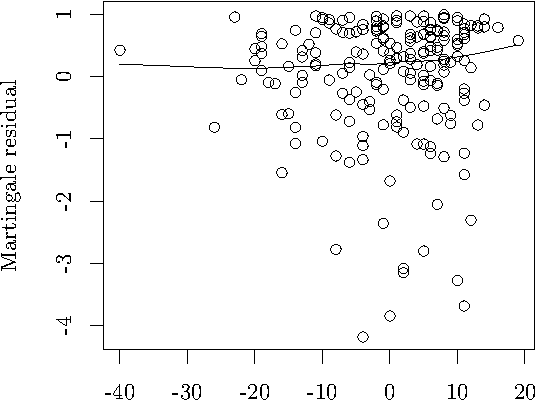
\includegraphics[width=\maxwidth]{figure/05-eda-func-form-age-1} 

}


\begin{kframe}\begin{alltt}
\hlkwd{scatter.smooth}\hlstd{(data}\hlopt{$}\hlstd{AgeCent,} \hlkwd{resid}\hlstd{(fit.cph.NoAge,} \hlkwc{type} \hlstd{=} \hlstr{"martingale"}\hlstd{),} \hlkwc{xlab} \hlstd{=} \hlstr{""}\hlstd{,} \hlkwc{ylab} \hlstd{=} \hlstr{"Martingale residual"}\hlstd{,} \hlkwc{ylim} \hlstd{=} \hlkwd{c}\hlstd{(}\hlopt{-}\hlnum{1}\hlstd{,} \hlnum{1}\hlstd{))}
\end{alltt}
\end{kframe}

{\centering 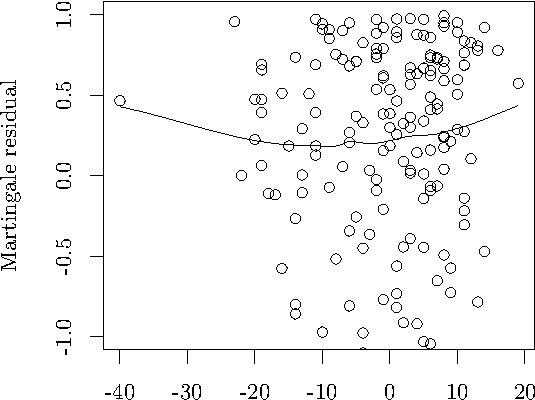
\includegraphics[width=\maxwidth]{figure/05-eda-func-form-age-2} 

}



\end{knitrout}

\begin{knitrout}
\definecolor{shadecolor}{rgb}{0.969, 0.969, 0.969}\color{fgcolor}\begin{kframe}
\begin{alltt}
\hlstd{fit.cph.NoSize} \hlkwb{=} \hlkwd{coxph}\hlstd{(}\hlkwd{Surv}\hlstd{(Time, DSD)} \hlopt{~} \hlstd{SexM} \hlopt{+} \hlstd{AgeCent} \hlopt{+} \hlstd{LocBody} \hlopt{+} \hlstd{A2} \hlopt{+} \hlstd{A4,} \hlkwc{data} \hlstd{= data)}
\hlkwd{scatter.smooth}\hlstd{(data}\hlopt{$}\hlstd{SizeCent,} \hlkwd{resid}\hlstd{(fit.cph.NoSize,} \hlkwc{type} \hlstd{=} \hlstr{"martingale"}\hlstd{),} \hlkwc{xlab} \hlstd{=} \hlstr{""}\hlstd{,} \hlkwc{ylab} \hlstd{=} \hlstr{"Martingale residual"}\hlstd{)}
\end{alltt}
\end{kframe}

{\centering 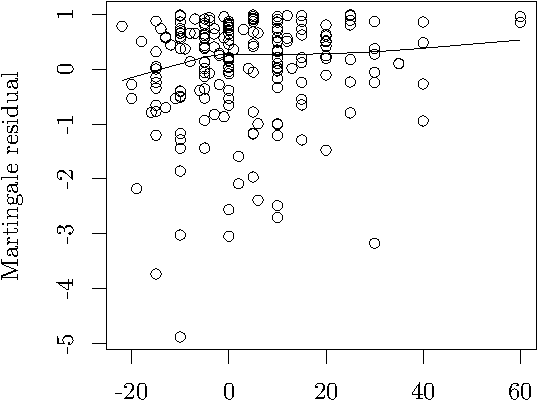
\includegraphics[width=\maxwidth]{figure/05-eda-func-form-size-1} 

}


\begin{kframe}\begin{alltt}
\hlkwd{scatter.smooth}\hlstd{(data}\hlopt{$}\hlstd{SizeCent,} \hlkwd{resid}\hlstd{(fit.cph.NoSize,} \hlkwc{type} \hlstd{=} \hlstr{"martingale"}\hlstd{),} \hlkwc{xlab} \hlstd{=} \hlstr{""}\hlstd{,} \hlkwc{ylab} \hlstd{=} \hlstr{"Martingale residual"}\hlstd{,} \hlkwc{ylim} \hlstd{=} \hlkwd{c}\hlstd{(}\hlopt{-}\hlnum{1}\hlstd{,} \hlnum{1}\hlstd{))}
\end{alltt}
\end{kframe}

{\centering 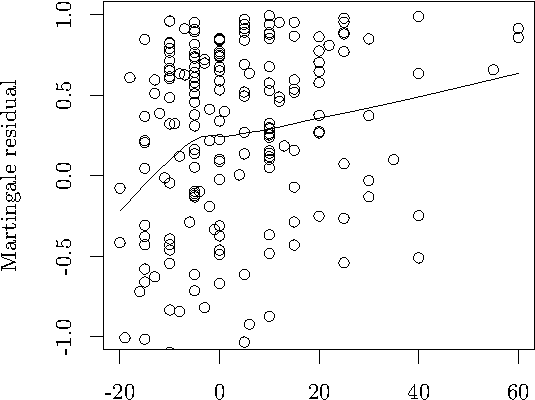
\includegraphics[width=\maxwidth]{figure/05-eda-func-form-size-2} 

}



\end{knitrout}
It looks like age has a minor nonlinear component, leading to a quadratic-like U shape.  The size relationship appears to have a knee, close to size == 0, around which the relationship is approximately linear.

Model age as:  $AgeCent + AgeCent^2$
Model size as: $SizeCent + SizeCent I(SizeCent > 0) \equiv SizeCent + SizeCent_+$

\begin{knitrout}
\definecolor{shadecolor}{rgb}{0.969, 0.969, 0.969}\color{fgcolor}\begin{kframe}
\begin{alltt}
\hlstd{data}\hlopt{$}\hlstd{SizeSmall} \hlkwb{=} \hlstd{data}\hlopt{$}\hlstd{SizeCent} \hlopt{*} \hlstd{(data}\hlopt{$}\hlstd{SizeCent} \hlopt{<} \hlnum{0}\hlstd{)}
\hlstd{data}\hlopt{$}\hlstd{AgeCent2} \hlkwb{=} \hlstd{data}\hlopt{$}\hlstd{AgeCent}\hlopt{^}\hlnum{2}
\end{alltt}
\end{kframe}
\end{knitrout}

\subsection{PH assumption: full model}
\begin{knitrout}
\definecolor{shadecolor}{rgb}{0.969, 0.969, 0.969}\color{fgcolor}\begin{kframe}
\begin{alltt}
\hlstd{fit.cph} \hlkwb{=} \hlkwd{coxph}\hlstd{(}\hlkwd{Surv}\hlstd{(Time, DSD)} \hlopt{~} \hlstd{SexM} \hlopt{+} \hlstd{AgeCent} \hlopt{+} \hlstd{AgeCent2} \hlopt{+} \hlstd{LocBody} \hlopt{+} \hlstd{SizeCent} \hlopt{+} \hlstd{SizeSmall} \hlopt{+} \hlstd{A2} \hlopt{+} \hlstd{A4,} \hlkwc{data} \hlstd{= data)}
\hlkwd{cox.zph}\hlstd{(fit.cph)}
\end{alltt}
\begin{verbatim}
##                 rho   chisq      p
## SexMTRUE     0.1571  4.2500 0.0393
## AgeCent     -0.0746  0.9839 0.3212
## AgeCent2     0.0391  0.2379 0.6258
## LocBodyTRUE -0.1295  2.6406 0.1042
## SizeCent     0.0074  0.0112 0.9157
## SizeSmall   -0.0575  0.6037 0.4372
## A2TRUE       0.0447  0.3555 0.5510
## A4TRUE      -0.0493  0.4172 0.5183
## GLOBAL           NA 12.8286 0.1179
\end{verbatim}
\begin{alltt}
\hlkwd{plot}\hlstd{(}\hlkwd{cox.zph}\hlstd{(fit.cph))}
\end{alltt}
\end{kframe}

{\centering 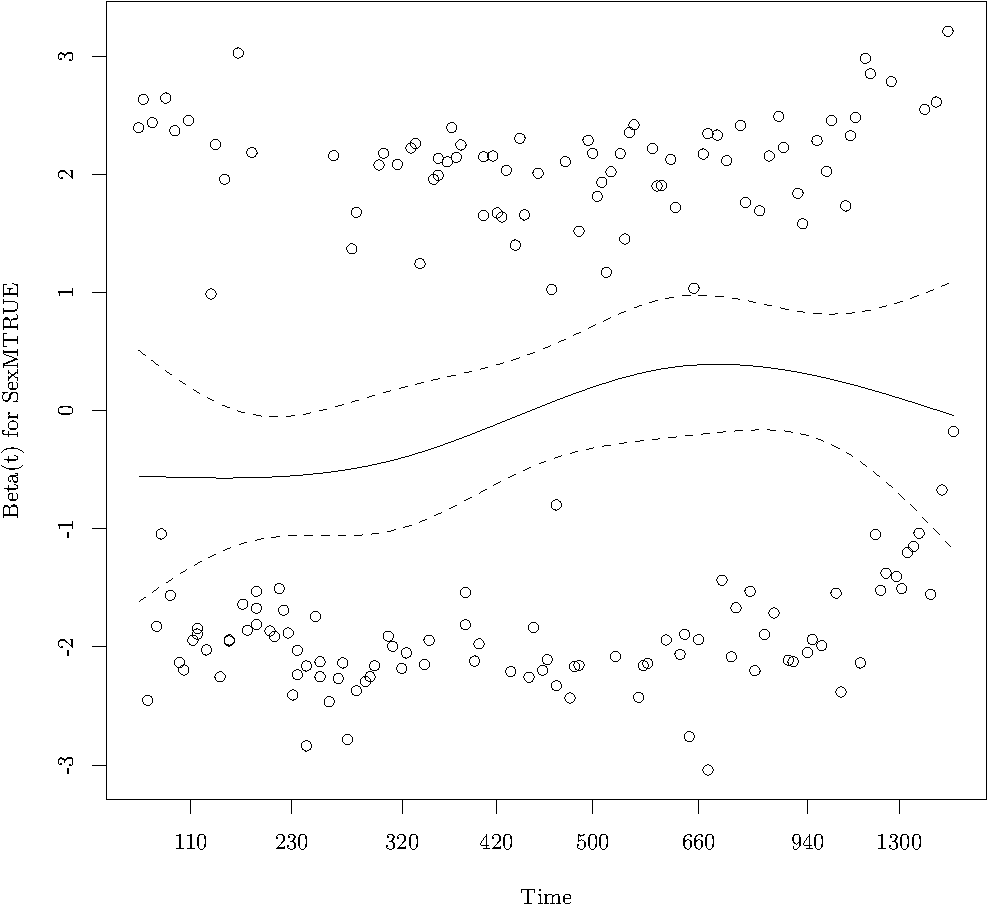
\includegraphics[width=\maxwidth]{figure/05-eda-ph-check-full-1} 

}




{\centering 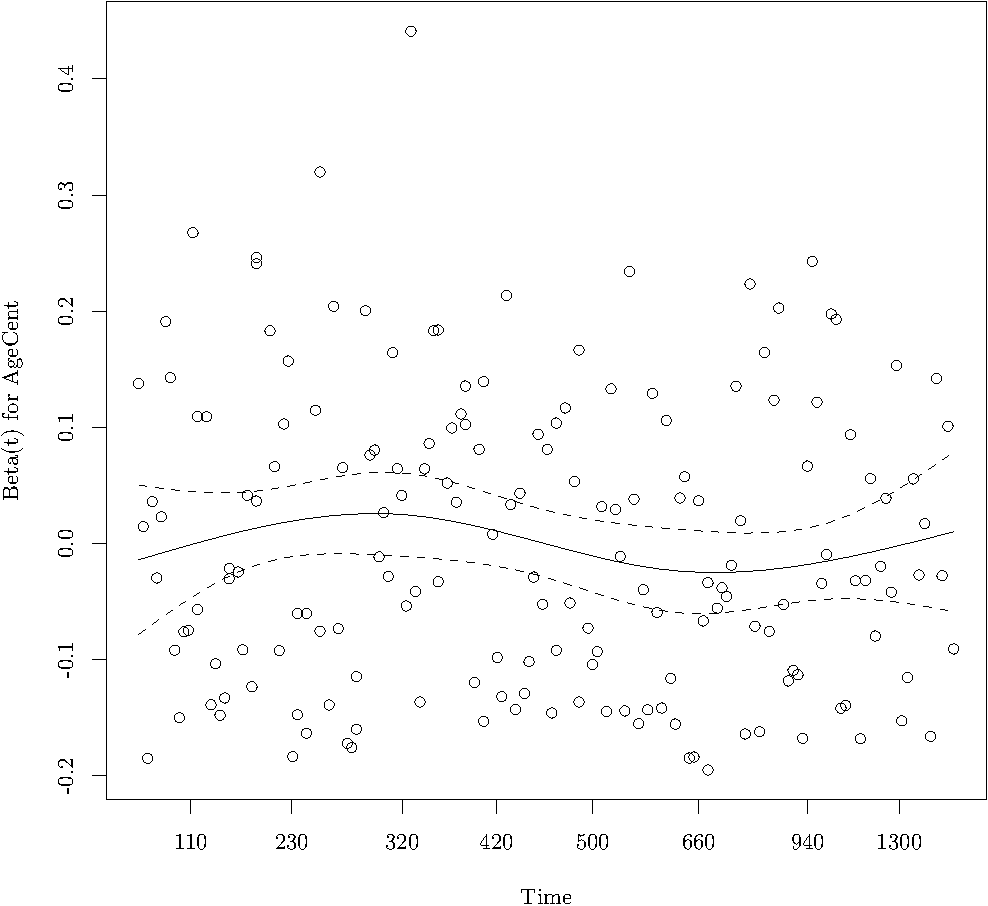
\includegraphics[width=\maxwidth]{figure/05-eda-ph-check-full-2} 

}




{\centering 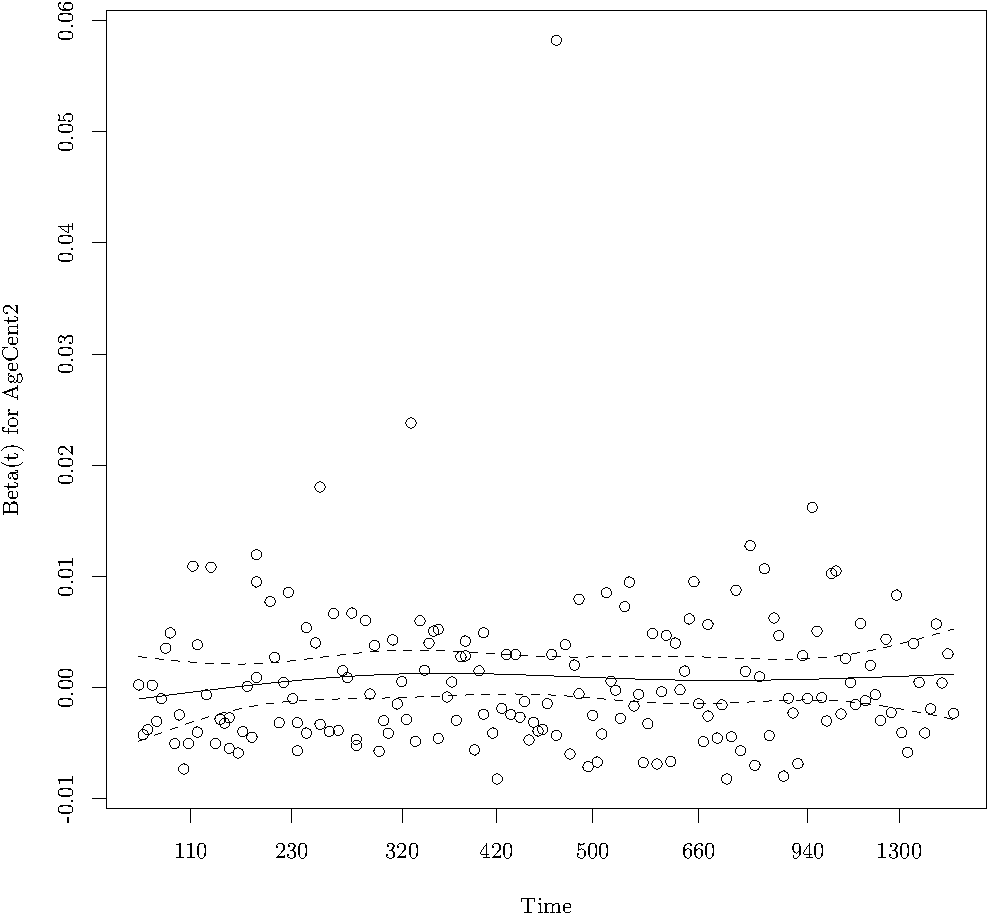
\includegraphics[width=\maxwidth]{figure/05-eda-ph-check-full-3} 

}




{\centering 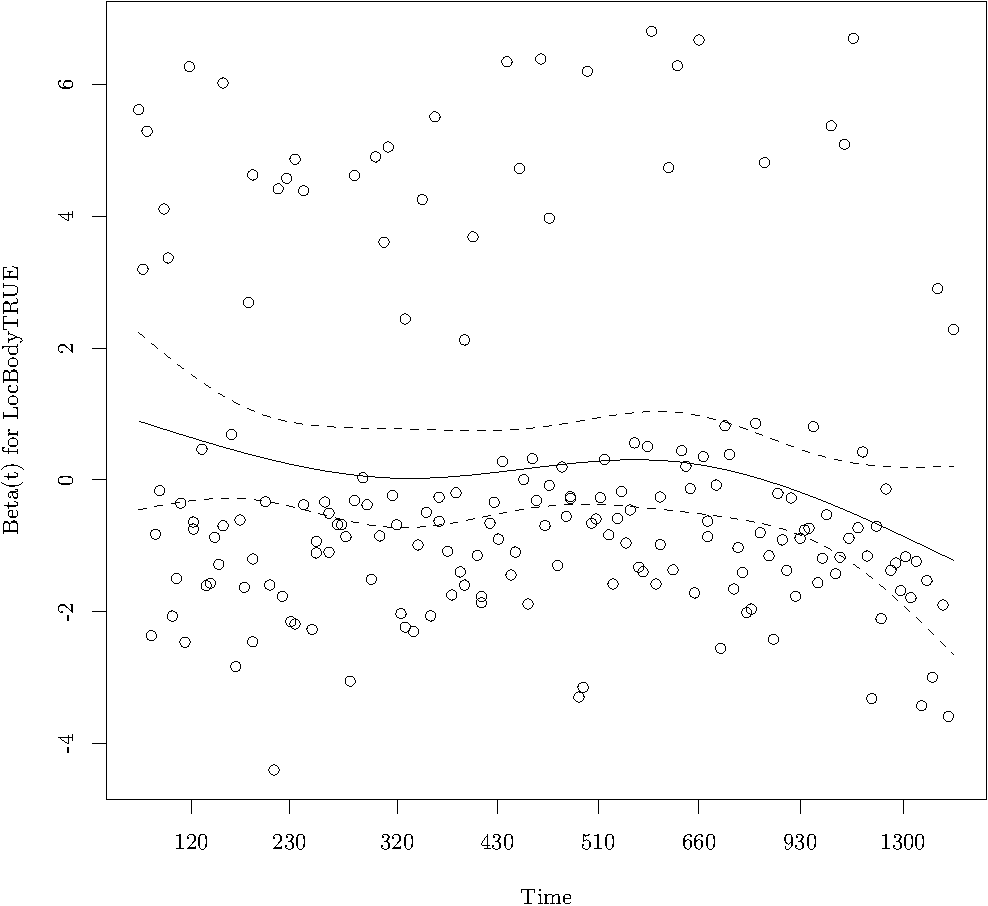
\includegraphics[width=\maxwidth]{figure/05-eda-ph-check-full-4} 

}




{\centering 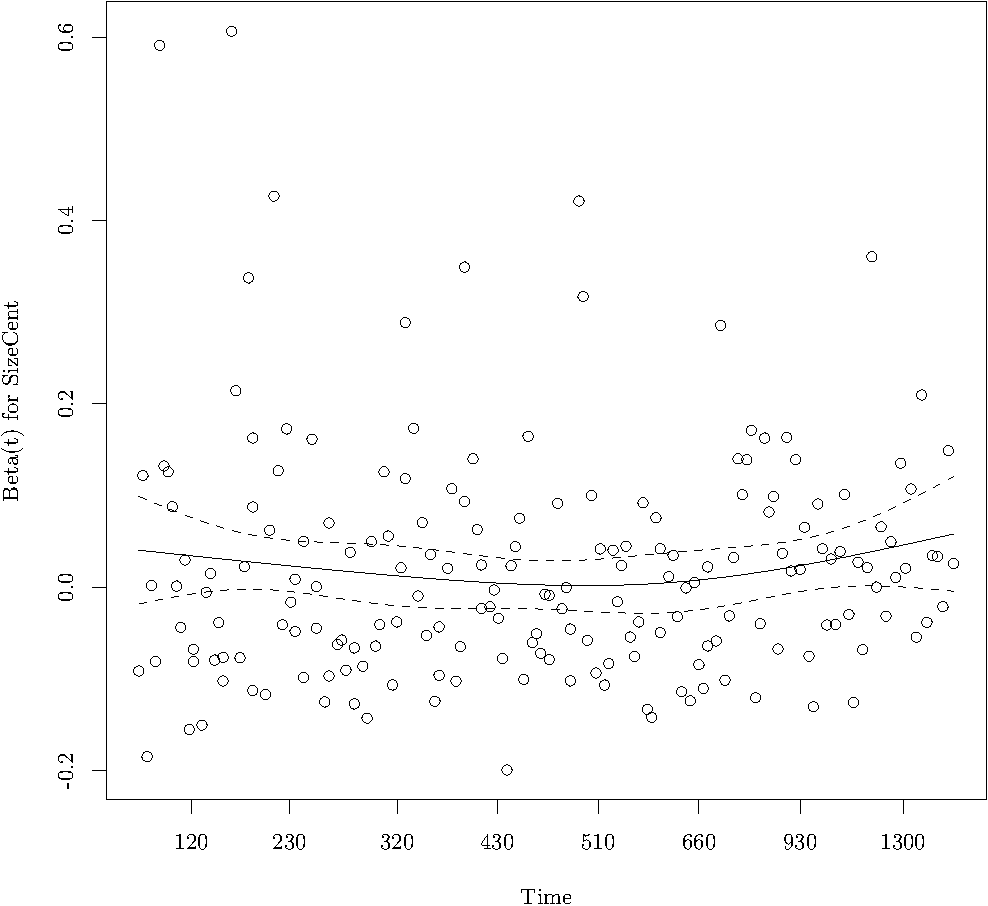
\includegraphics[width=\maxwidth]{figure/05-eda-ph-check-full-5} 

}




{\centering 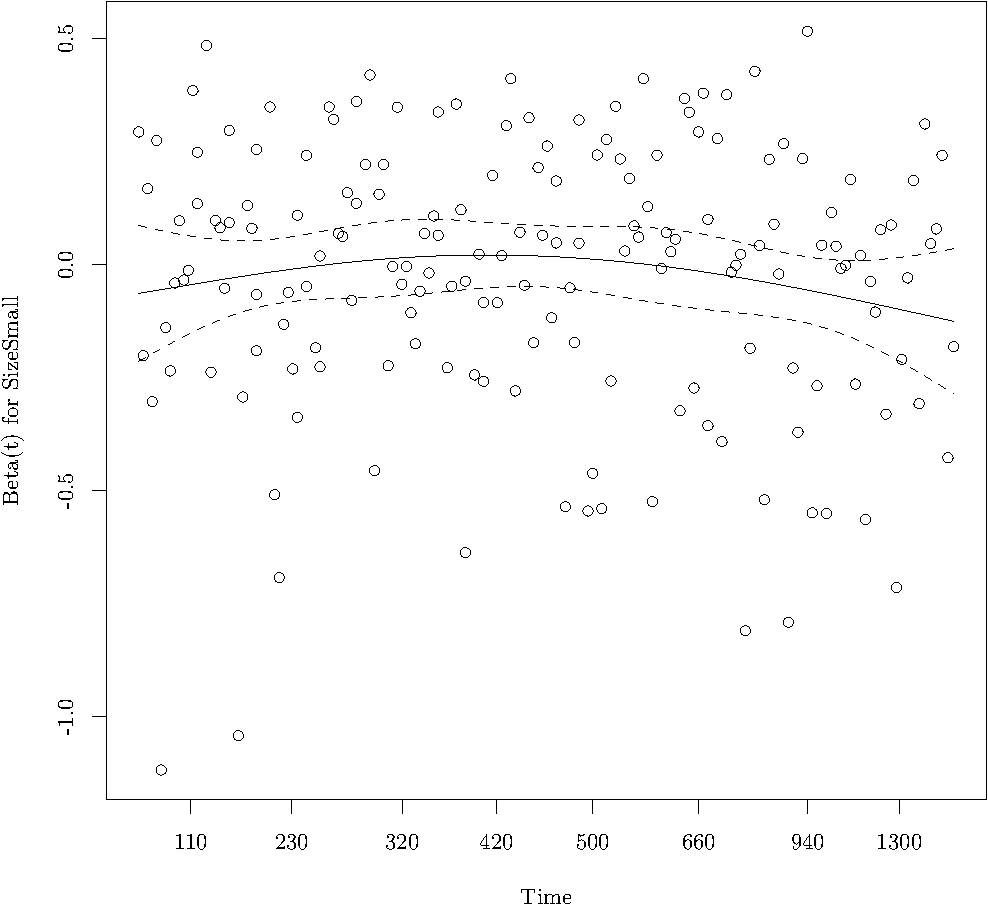
\includegraphics[width=\maxwidth]{figure/05-eda-ph-check-full-6} 

}




{\centering 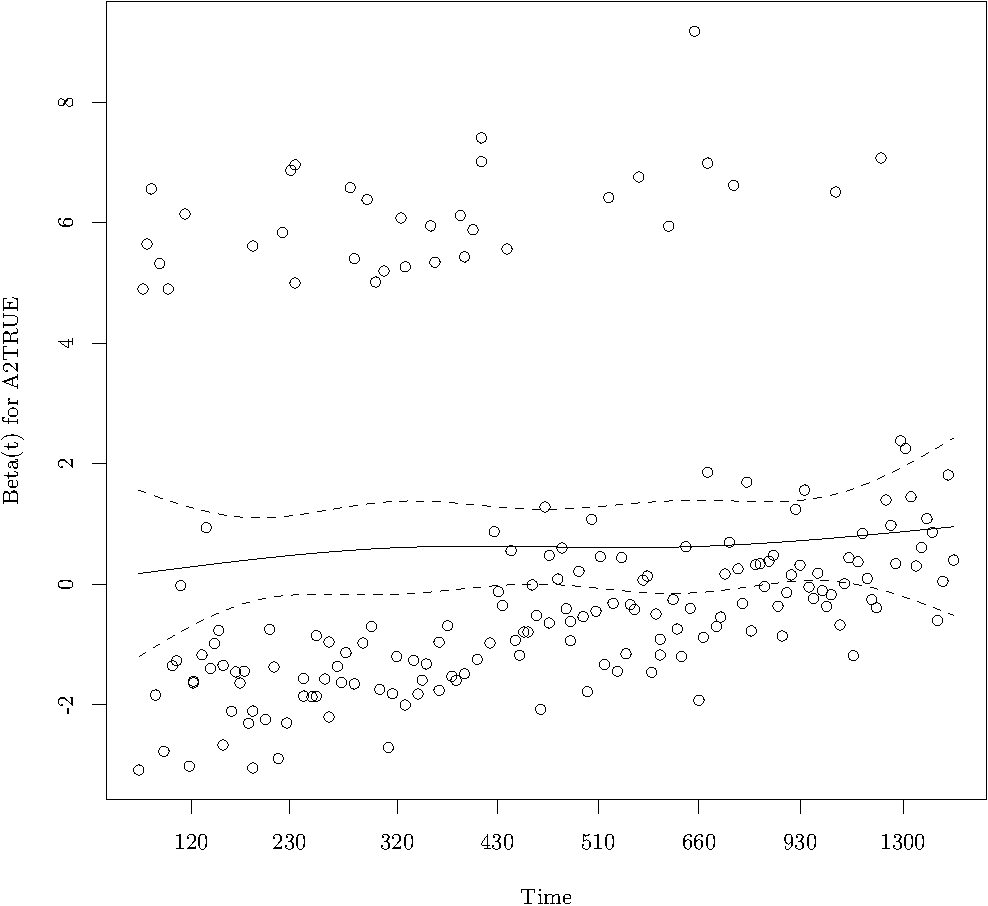
\includegraphics[width=\maxwidth]{figure/05-eda-ph-check-full-7} 

}




{\centering 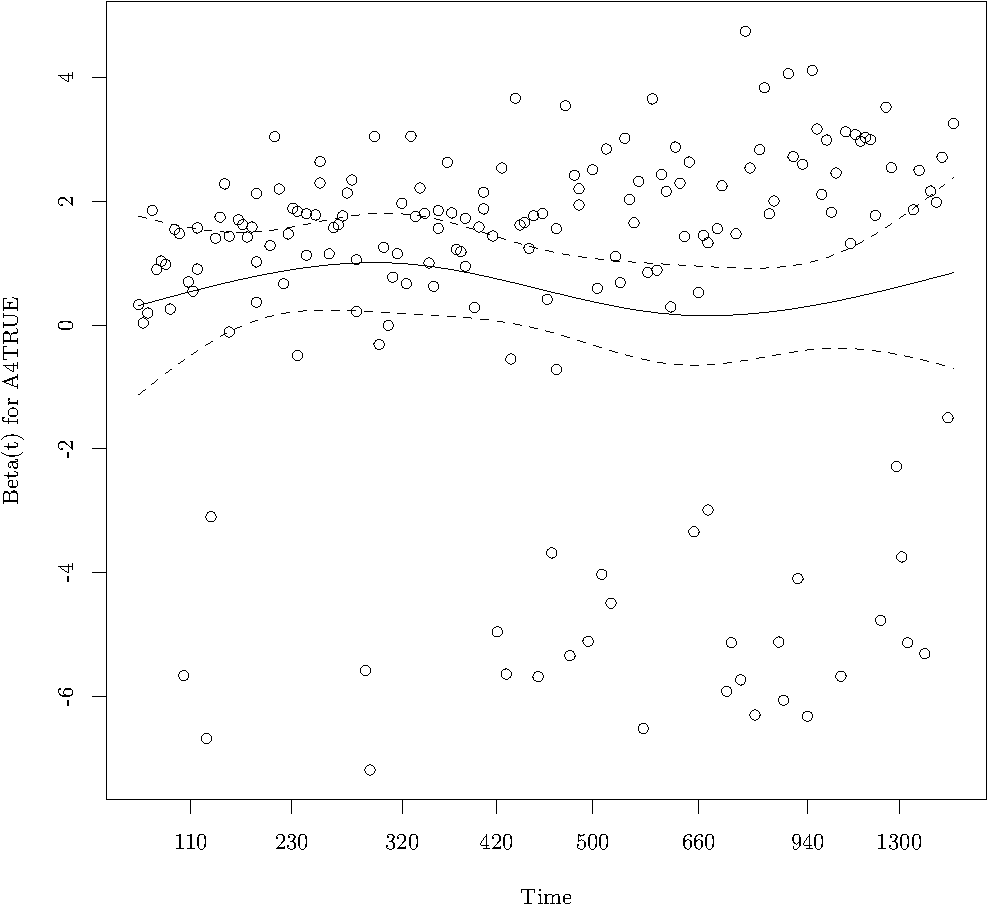
\includegraphics[width=\maxwidth]{figure/05-eda-ph-check-full-8} 

}



\end{knitrout}

\begin{knitrout}
\definecolor{shadecolor}{rgb}{0.969, 0.969, 0.969}\color{fgcolor}\begin{kframe}
\begin{alltt}
\hlstd{temp} \hlkwb{=} \hlkwa{function} \hlstd{(}\hlkwc{x}\hlstd{,} \hlkwc{resid} \hlstd{=} \hlnum{TRUE}\hlstd{,} \hlkwc{se} \hlstd{=} \hlnum{TRUE}\hlstd{,} \hlkwc{df} \hlstd{=} \hlnum{4}\hlstd{,} \hlkwc{nsmo} \hlstd{=} \hlnum{40}\hlstd{,} \hlkwc{var}\hlstd{,} \hlkwc{...}\hlstd{) \{}
    \hlstd{xx} \hlkwb{<-} \hlstd{x}\hlopt{$}\hlstd{x}
    \hlstd{yy} \hlkwb{<-} \hlstd{x}\hlopt{$}\hlstd{y}
    \hlstd{d} \hlkwb{<-} \hlkwd{nrow}\hlstd{(yy)}
    \hlstd{df} \hlkwb{<-} \hlkwd{max}\hlstd{(df)}
    \hlstd{nvar} \hlkwb{<-} \hlkwd{ncol}\hlstd{(yy)}
    \hlstd{pred.x} \hlkwb{<-} \hlkwd{seq}\hlstd{(}\hlkwc{from} \hlstd{=} \hlkwd{min}\hlstd{(xx),} \hlkwc{to} \hlstd{=} \hlkwd{max}\hlstd{(xx),} \hlkwc{length} \hlstd{= nsmo)}
    \hlstd{temp} \hlkwb{<-} \hlkwd{c}\hlstd{(pred.x, xx)}
    \hlstd{lmat} \hlkwb{<-} \hlkwd{ns}\hlstd{(temp,} \hlkwc{df} \hlstd{= df,} \hlkwc{intercept} \hlstd{=} \hlnum{TRUE}\hlstd{)}
    \hlstd{pmat} \hlkwb{<-} \hlstd{lmat[}\hlnum{1}\hlopt{:}\hlstd{nsmo, ]}
    \hlstd{xmat} \hlkwb{<-} \hlstd{lmat[}\hlopt{-}\hlstd{(}\hlnum{1}\hlopt{:}\hlstd{nsmo), ]}
    \hlstd{qmat} \hlkwb{<-} \hlkwd{qr}\hlstd{(xmat)}
    \hlkwa{if} \hlstd{(qmat}\hlopt{$}\hlstd{rank} \hlopt{<} \hlstd{df)}
        \hlkwd{stop}\hlstd{(}\hlstr{"Spline fit is singular, try a smaller degrees of freedom"}\hlstd{)}
    \hlkwa{if} \hlstd{(se) \{}
        \hlstd{bk} \hlkwb{<-} \hlkwd{backsolve}\hlstd{(qmat}\hlopt{$}\hlstd{qr[}\hlnum{1}\hlopt{:}\hlstd{df,} \hlnum{1}\hlopt{:}\hlstd{df],} \hlkwd{diag}\hlstd{(df))}
        \hlstd{xtx} \hlkwb{<-} \hlstd{bk} \hlopt \hlkwd{t}\hlstd{(bk)}
        \hlstd{seval} \hlkwb{<-} \hlstd{d} \hlopt{*} \hlstd{((pmat} \hlopt \hlstd{xtx)} \hlopt{*} \hlstd{pmat)} \hlopt \hlkwd{rep}\hlstd{(}\hlnum{1}\hlstd{, df)}
    \hlstd{\}}
    \hlstd{ylab} \hlkwb{<-} \hlkwd{paste}\hlstd{(}\hlstr{"Beta(t) for"}\hlstd{,} \hlkwd{dimnames}\hlstd{(yy)[[}\hlnum{2}\hlstd{]])}
    \hlkwa{if} \hlstd{(}\hlkwd{missing}\hlstd{(var))}
        \hlstd{var} \hlkwb{<-} \hlnum{1}\hlopt{:}\hlstd{nvar}
    \hlkwa{else} \hlstd{\{}
        \hlkwa{if} \hlstd{(}\hlkwd{is.character}\hlstd{(var))}
            \hlstd{var} \hlkwb{<-} \hlkwd{match}\hlstd{(var,} \hlkwd{dimnames}\hlstd{(yy)[[}\hlnum{2}\hlstd{]])}
        \hlkwa{if} \hlstd{(}\hlkwd{any}\hlstd{(}\hlkwd{is.na}\hlstd{(var))} \hlopt{||} \hlkwd{max}\hlstd{(var)} \hlopt{>} \hlstd{nvar} \hlopt{||} \hlkwd{min}\hlstd{(var)} \hlopt{<}
            \hlnum{1}\hlstd{)}
            \hlkwd{stop}\hlstd{(}\hlstr{"Invalid variable requested"}\hlstd{)}
    \hlstd{\}}
    \hlkwa{if} \hlstd{(x}\hlopt{$}\hlstd{transform} \hlopt{==} \hlstr{"log"}\hlstd{) \{}
        \hlstd{xx} \hlkwb{<-} \hlkwd{exp}\hlstd{(xx)}
        \hlstd{pred.x} \hlkwb{<-} \hlkwd{exp}\hlstd{(pred.x)}
    \hlstd{\}}
    \hlkwa{else if} \hlstd{(x}\hlopt{$}\hlstd{transform} \hlopt{!=} \hlstr{"identity"}\hlstd{) \{}
        \hlstd{xtime} \hlkwb{<-} \hlkwd{as.numeric}\hlstd{(}\hlkwd{dimnames}\hlstd{(yy)[[}\hlnum{1}\hlstd{]])}
        \hlstd{indx} \hlkwb{<-} \hlopt{!}\hlkwd{duplicated}\hlstd{(xx)}
        \hlstd{apr1} \hlkwb{<-} \hlkwd{approx}\hlstd{(xx[indx], xtime[indx],} \hlkwd{seq}\hlstd{(}\hlkwd{min}\hlstd{(xx),} \hlkwd{max}\hlstd{(xx),}
            \hlkwc{length} \hlstd{=} \hlnum{17}\hlstd{)[}\hlnum{2} \hlopt{*} \hlstd{(}\hlnum{1}\hlopt{:}\hlnum{8}\hlstd{)])}
        \hlstd{temp} \hlkwb{<-} \hlkwd{signif}\hlstd{(apr1}\hlopt{$}\hlstd{y,} \hlnum{2}\hlstd{)}
        \hlstd{apr2} \hlkwb{<-} \hlkwd{approx}\hlstd{(xtime[indx], xx[indx], temp)}
        \hlstd{xaxisval} \hlkwb{<-} \hlstd{apr2}\hlopt{$}\hlstd{y}
        \hlstd{xaxislab} \hlkwb{<-} \hlkwd{rep}\hlstd{(}\hlstr{""}\hlstd{,} \hlnum{8}\hlstd{)}
        \hlkwa{for} \hlstd{(i} \hlkwa{in} \hlnum{1}\hlopt{:}\hlnum{8}\hlstd{) xaxislab[i]} \hlkwb{<-} \hlkwd{format}\hlstd{(temp[i])}
    \hlstd{\}}
    \hlkwa{for} \hlstd{(i} \hlkwa{in} \hlstd{var) \{}
        \hlstd{y} \hlkwb{<-} \hlstd{yy[, i]}
        \hlstd{yhat} \hlkwb{<-} \hlstd{pmat} \hlopt \hlkwd{qr.coef}\hlstd{(qmat, y)}
        \hlkwa{if} \hlstd{(resid)}
            \hlstd{yr} \hlkwb{<-} \hlkwd{range}\hlstd{(yhat, y)}
        \hlkwa{else} \hlstd{yr} \hlkwb{<-} \hlkwd{range}\hlstd{(yhat)}
        \hlkwa{if} \hlstd{(se) \{}
            \hlstd{temp} \hlkwb{<-} \hlnum{2} \hlopt{*} \hlkwd{sqrt}\hlstd{(x}\hlopt{$}\hlstd{var[i, i]} \hlopt{*} \hlstd{seval)}
            \hlstd{yup} \hlkwb{<-} \hlstd{yhat} \hlopt{+} \hlstd{temp}
            \hlstd{ylow} \hlkwb{<-} \hlstd{yhat} \hlopt{-} \hlstd{temp}
            \hlstd{yr} \hlkwb{<-} \hlkwd{range}\hlstd{(yr, yup, ylow)}
        \hlstd{\}}
        \hlkwa{if} \hlstd{(x}\hlopt{$}\hlstd{transform} \hlopt{==} \hlstr{"identity"}\hlstd{)}
            \hlkwd{plot}\hlstd{(}\hlkwd{range}\hlstd{(xx), yr,} \hlkwc{type} \hlstd{=} \hlstr{"n"}\hlstd{, ...)}
        \hlkwa{else if} \hlstd{(x}\hlopt{$}\hlstd{transform} \hlopt{==} \hlstr{"log"}\hlstd{)}
            \hlkwd{plot}\hlstd{(}\hlkwd{range}\hlstd{(xx), yr,} \hlkwc{type} \hlstd{=} \hlstr{"n"}\hlstd{,} \hlkwc{log} \hlstd{=} \hlstr{"x"}\hlstd{, ...)}
        \hlkwa{else} \hlstd{\{}
            \hlkwd{plot}\hlstd{(}\hlkwd{range}\hlstd{(xx), yr,} \hlkwc{type} \hlstd{=} \hlstr{"n"}\hlstd{,} \hlkwc{axes} \hlstd{=} \hlnum{FALSE}\hlstd{, ...)}
            \hlkwd{axis}\hlstd{(}\hlnum{1}\hlstd{, xaxisval, xaxislab)}
            \hlkwd{axis}\hlstd{(}\hlnum{2}\hlstd{)}
            \hlkwd{box}\hlstd{()}
        \hlstd{\}}
        \hlkwa{if} \hlstd{(resid)}
            \hlkwd{points}\hlstd{(xx, y)}
        \hlkwd{lines}\hlstd{(pred.x, yhat)}
        \hlkwa{if} \hlstd{(se) \{}
            \hlkwd{lines}\hlstd{(pred.x, yup,} \hlkwc{lty} \hlstd{=} \hlnum{2}\hlstd{)}
            \hlkwd{lines}\hlstd{(pred.x, ylow,} \hlkwc{lty} \hlstd{=} \hlnum{2}\hlstd{)}
        \hlstd{\}}
    \hlstd{\}}
\hlstd{\}}

\hlkwd{temp}\hlstd{(}\hlkwd{cox.zph}\hlstd{(fit.cph),} \hlkwc{var} \hlstd{=} \hlnum{1}\hlstd{,} \hlkwc{ylab} \hlstd{=} \hlstr{"Scaled Schoenfeld residual for patient sex"}\hlstd{,} \hlkwc{xlab} \hlstd{=} \hlstr{"Time"}\hlstd{)}
\hlkwd{abline}\hlstd{(}\hlkwc{h} \hlstd{=} \hlnum{0}\hlstd{,} \hlkwc{lty} \hlstd{=} \hlstr{"dotted"}\hlstd{)}
\end{alltt}
\end{kframe}

{\centering 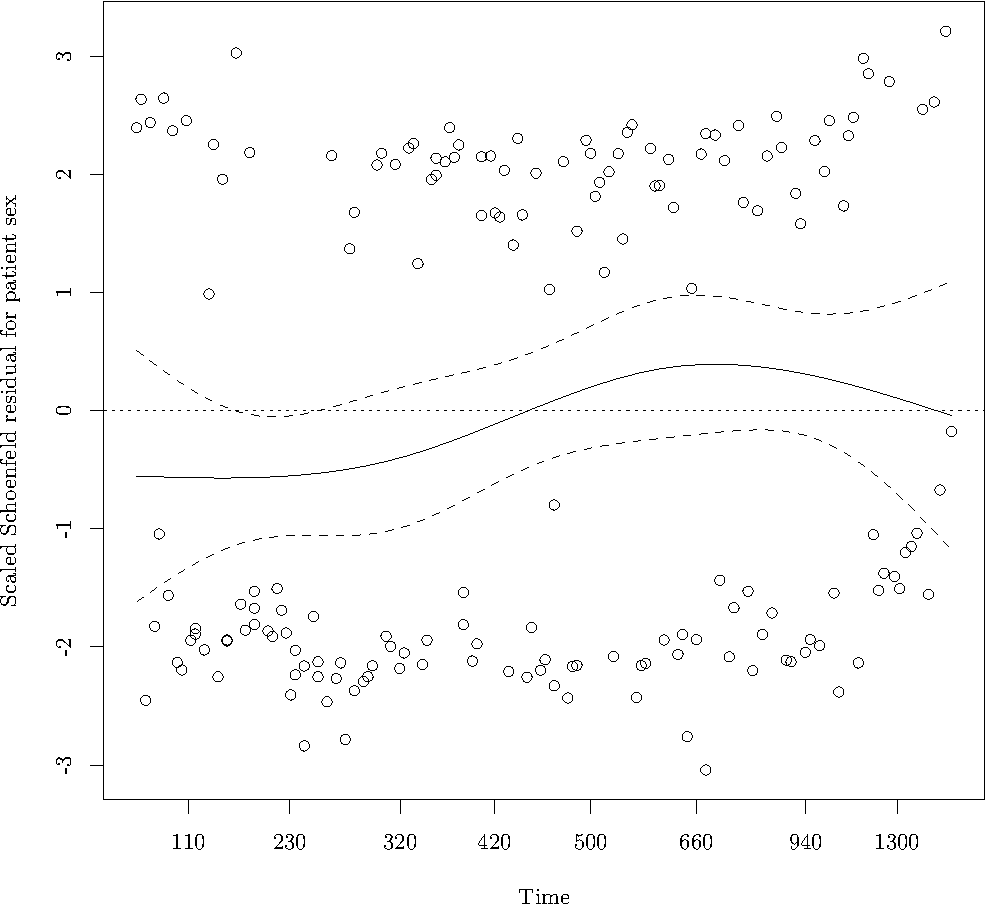
\includegraphics[width=\maxwidth]{figure/05-eda-ph-check-full-sexplot-1} 

}



\end{knitrout}


Looks like there's a violation of CPH with gender.  Not unexpected.  First check whether there is any evidence of gender interaction.
\begin{knitrout}
\definecolor{shadecolor}{rgb}{0.969, 0.969, 0.969}\color{fgcolor}\begin{kframe}
\begin{alltt}
\hlkwd{anova}\hlstd{(}\hlkwd{coxph}\hlstd{(}\hlkwd{Surv}\hlstd{(Time, DSD)} \hlopt{~} \hlstd{SexM}\hlopt{*}\hlstd{(AgeCent} \hlopt{+} \hlstd{AgeCent2} \hlopt{+} \hlstd{LocBody} \hlopt{+} \hlstd{SizeCent} \hlopt{+} \hlstd{SizeSmall} \hlopt{+} \hlstd{A2} \hlopt{+} \hlstd{A4),} \hlkwc{data} \hlstd{= data))}
\end{alltt}
\begin{verbatim}
## Analysis of Deviance Table
##  Cox model: response is Surv(Time, DSD)
## Terms added sequentially (first to last)
## 
##                loglik Chisq Df Pr(>|Chi|)
## NULL             -748                    
## SexM             -748  0.51  1     0.4762
## AgeCent          -747  0.19  1     0.6625
## AgeCent2         -747  0.81  1     0.3694
## LocBody          -746  2.40  1     0.1215
## SizeCent         -742  6.82  1     0.0090
## SizeSmall        -742  0.00  1     0.9563
## A2               -738  9.50  1     0.0021
## A4               -734  8.18  1     0.0042
## SexM:AgeCent     -733  0.37  1     0.5408
## SexM:AgeCent2    -733  0.17  1     0.6822
## SexM:LocBody     -733  0.09  1     0.7654
## SexM:SizeCent    -733  0.35  1     0.5568
## SexM:SizeSmall   -733  0.06  1     0.8068
## SexM:A2          -733  0.00  1     0.9588
## SexM:A4          -733  0.06  1     0.8000
\end{verbatim}
\end{kframe}
\end{knitrout}
Nope, good.  We're not interested in gender effects so just stratify.

\begin{knitrout}
\definecolor{shadecolor}{rgb}{0.969, 0.969, 0.969}\color{fgcolor}\begin{kframe}
\begin{alltt}
\hlstd{fit.cph} \hlkwb{=} \hlkwd{coxph}\hlstd{(}\hlkwd{Surv}\hlstd{(Time, DSD)} \hlopt{~} \hlkwd{strata}\hlstd{(SexM)} \hlopt{+} \hlstd{AgeCent} \hlopt{+} \hlstd{AgeCent2} \hlopt{+} \hlstd{LocBody} \hlopt{+} \hlstd{SizeCent} \hlopt{+} \hlstd{SizeSmall} \hlopt{+} \hlstd{A2} \hlopt{+} \hlstd{A4,} \hlkwc{data} \hlstd{= data)}
\hlkwd{cox.zph}\hlstd{(fit.cph)}
\end{alltt}
\begin{verbatim}
##                  rho   chisq     p
## AgeCent     -0.07987 1.18163 0.277
## AgeCent2     0.03673 0.20762 0.649
## LocBodyTRUE -0.10954 1.84364 0.175
## SizeCent    -0.00689 0.00961 0.922
## SizeSmall   -0.04493 0.36247 0.547
## A2TRUE       0.04775 0.40111 0.527
## A4TRUE      -0.05491 0.51655 0.472
## GLOBAL            NA 6.85340 0.444
\end{verbatim}
\begin{alltt}
\hlkwd{plot}\hlstd{(}\hlkwd{cox.zph}\hlstd{(fit.cph))}
\end{alltt}
\end{kframe}

{\centering 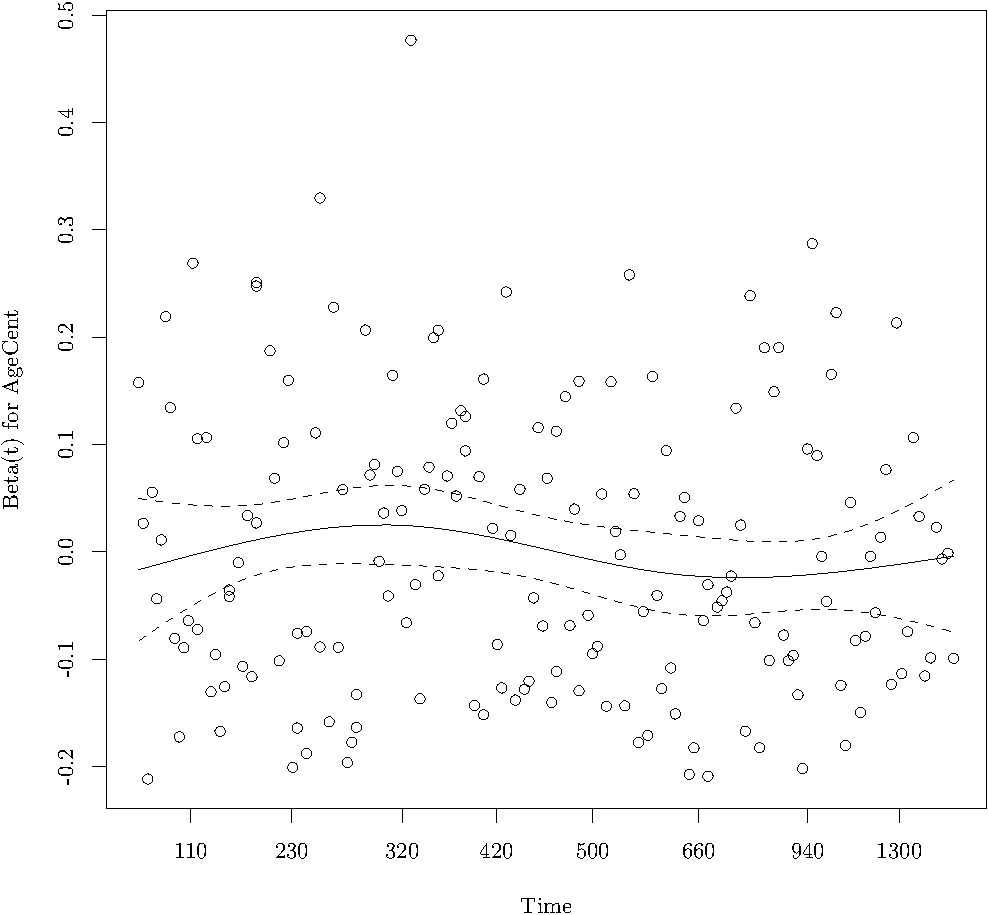
\includegraphics[width=\maxwidth]{figure/05-eda-ph-check-full-3-1} 

}




{\centering 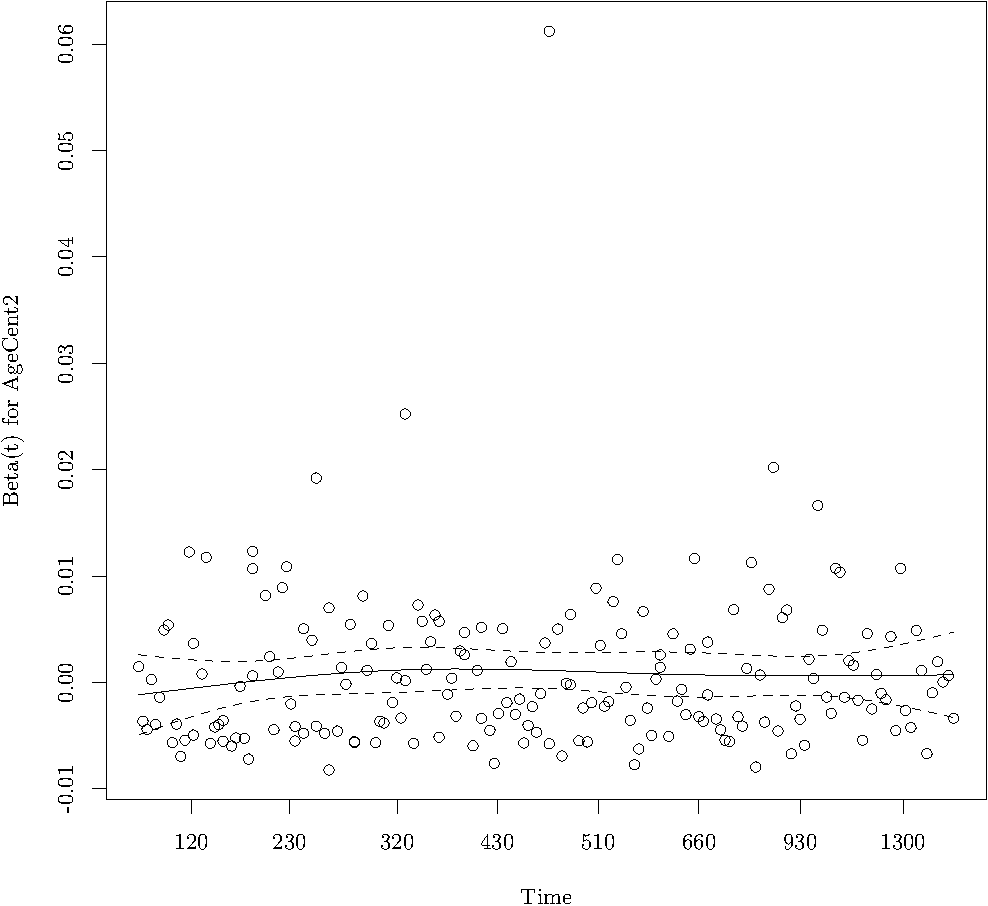
\includegraphics[width=\maxwidth]{figure/05-eda-ph-check-full-3-2} 

}




{\centering 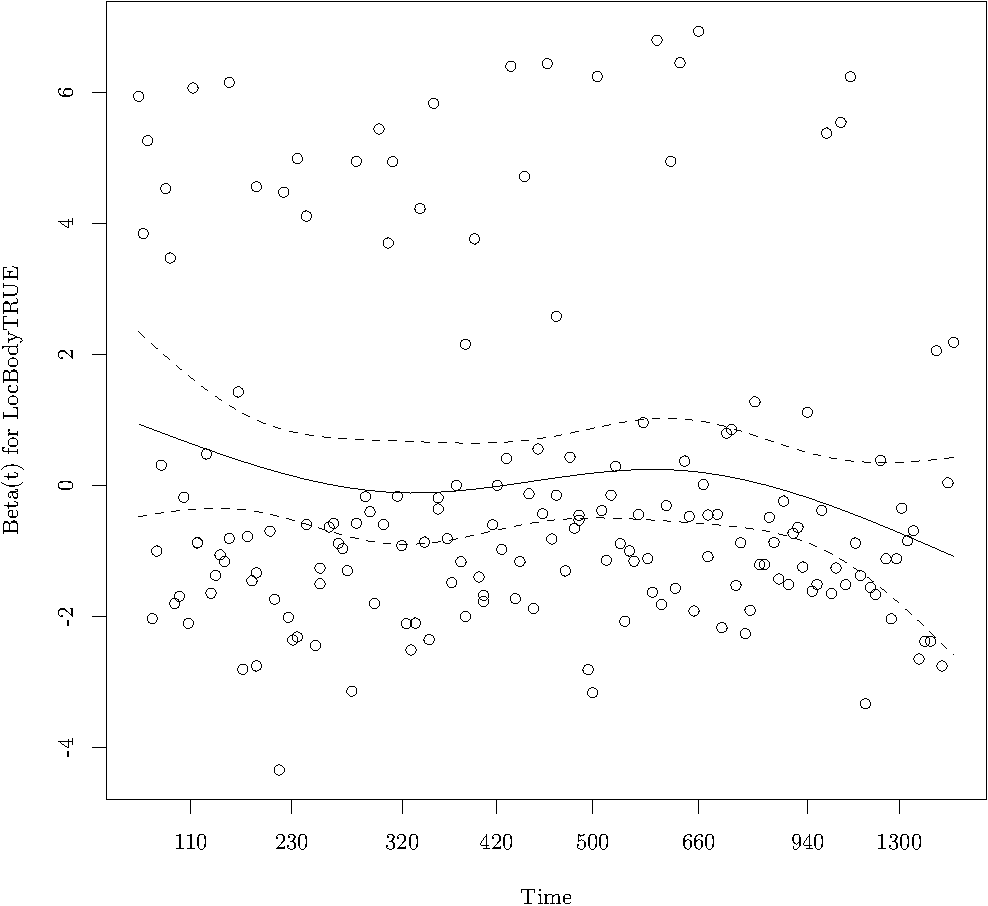
\includegraphics[width=\maxwidth]{figure/05-eda-ph-check-full-3-3} 

}




{\centering 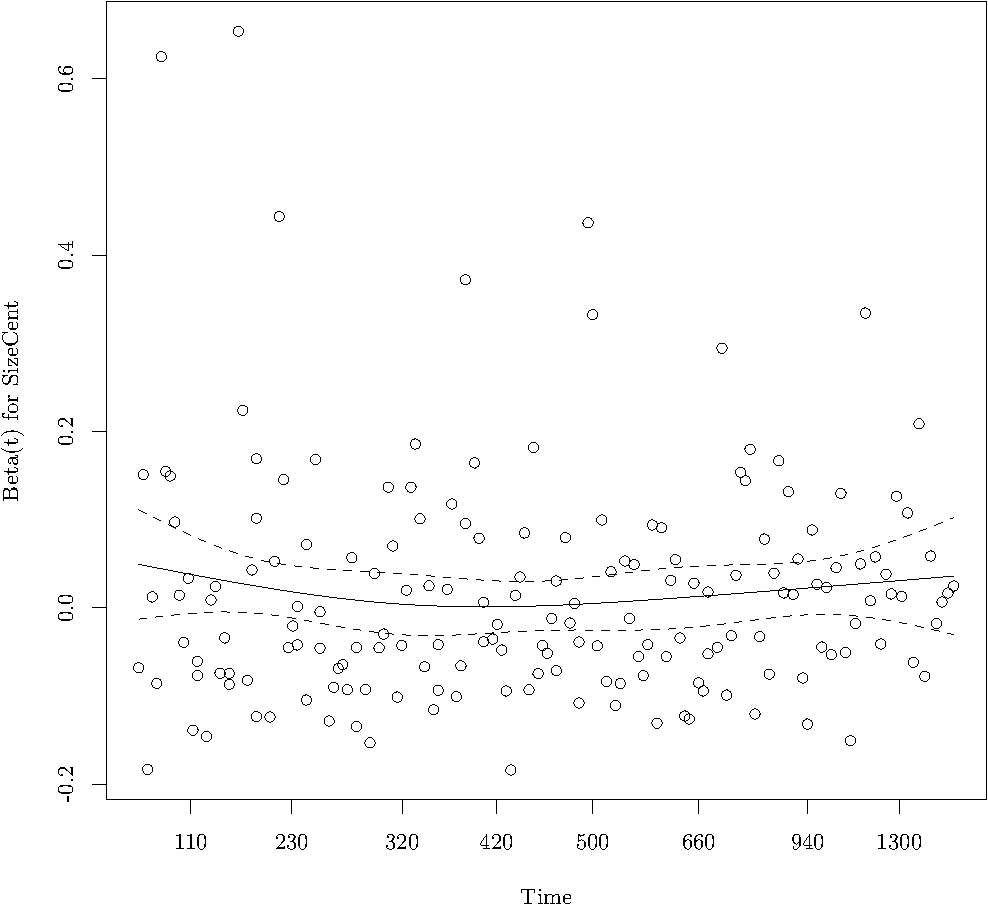
\includegraphics[width=\maxwidth]{figure/05-eda-ph-check-full-3-4} 

}




{\centering 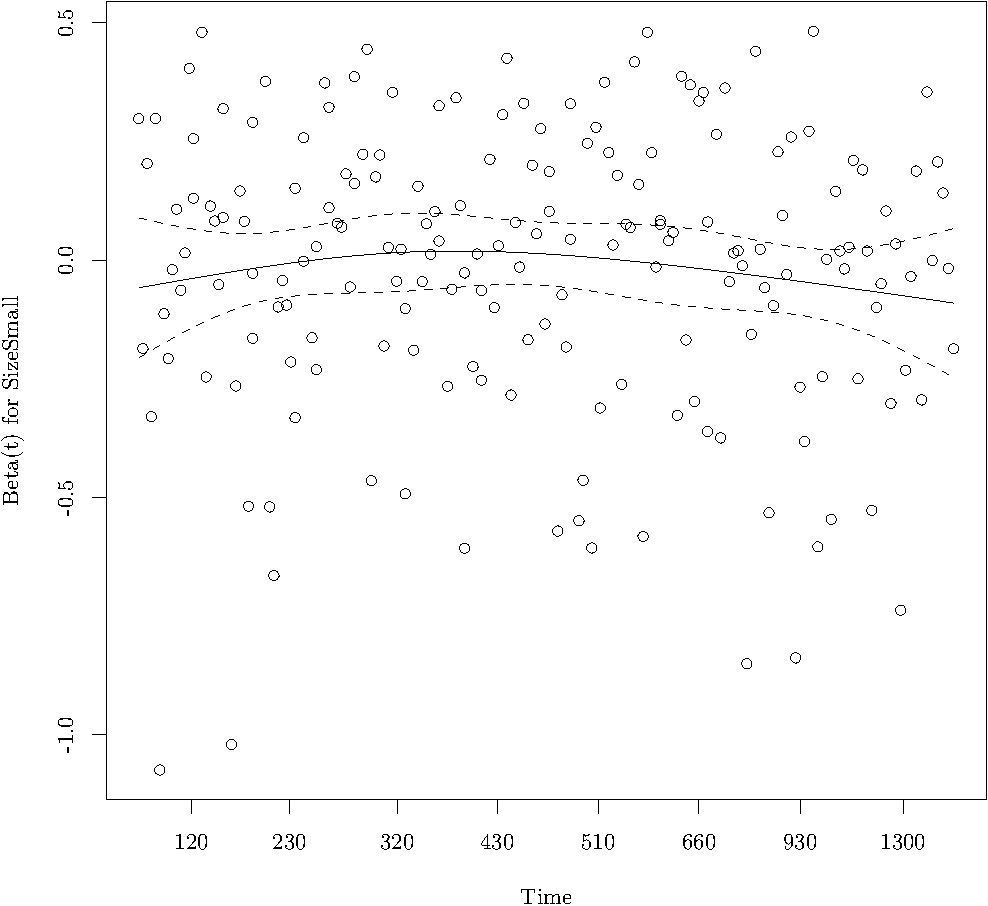
\includegraphics[width=\maxwidth]{figure/05-eda-ph-check-full-3-5} 

}




{\centering 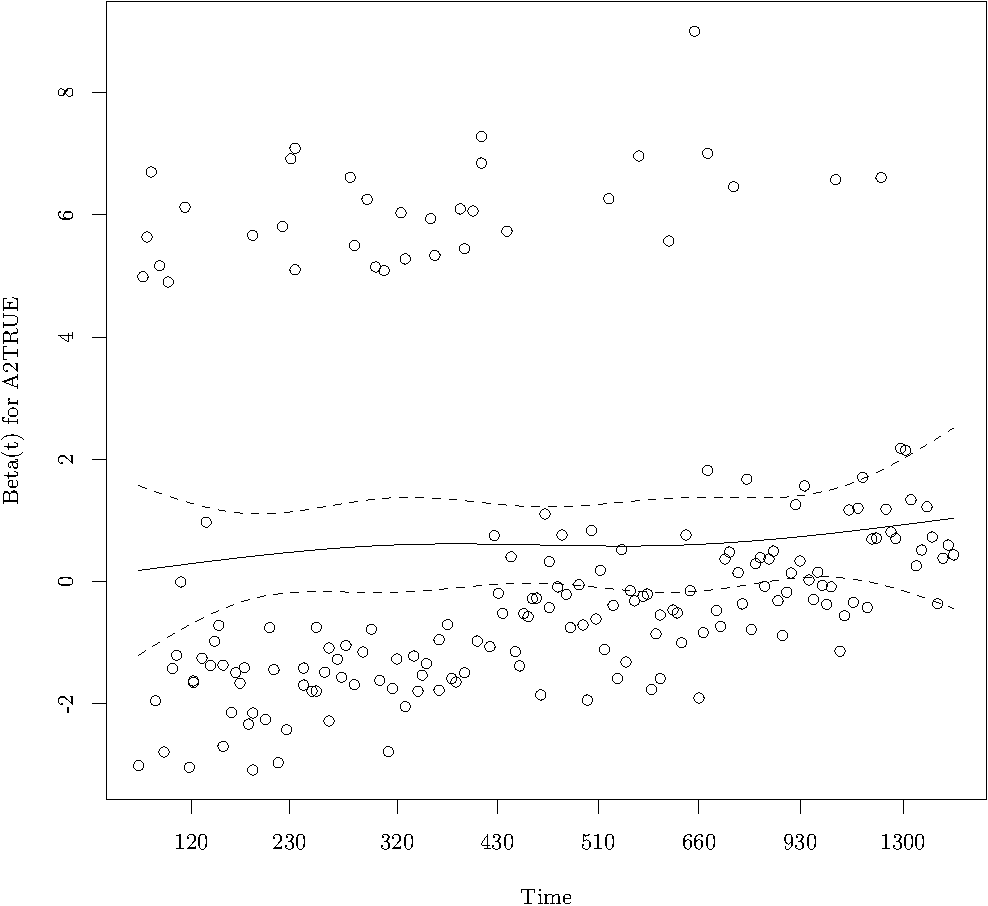
\includegraphics[width=\maxwidth]{figure/05-eda-ph-check-full-3-6} 

}




{\centering 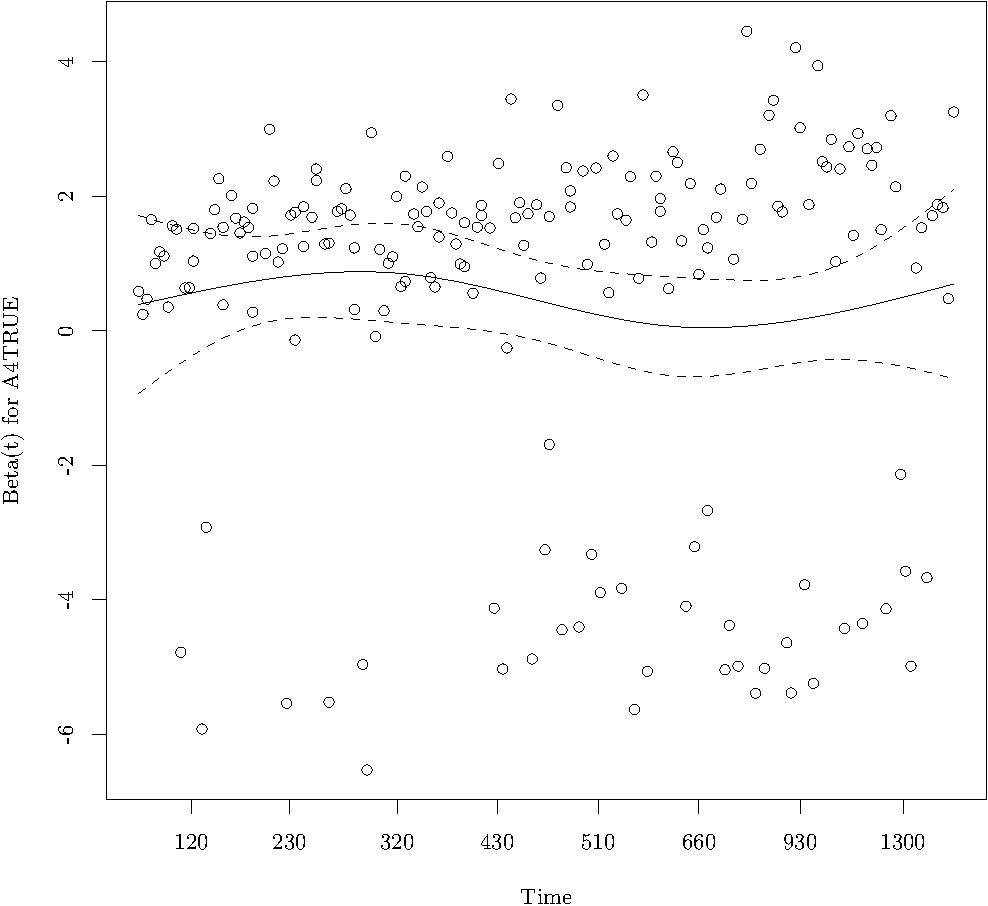
\includegraphics[width=\maxwidth]{figure/05-eda-ph-check-full-3-7} 

}



\end{knitrout}

Looks good.  Slight snifter with age but I'm not particularly concerned.
Split into age groups and do KM plots to verify.
\begin{knitrout}
\definecolor{shadecolor}{rgb}{0.969, 0.969, 0.969}\color{fgcolor}\begin{kframe}
\begin{alltt}
\hlstd{temp.age} \hlkwb{=} \hlkwd{cut}\hlstd{(data}\hlopt{$}\hlstd{AgeCent,} \hlnum{4}\hlstd{)}
\hlstd{temp} \hlkwb{=} \hlkwd{survfit}\hlstd{(}\hlkwd{Surv}\hlstd{(Time, DSD)} \hlopt{~} \hlstd{temp.age, data)}
\hlkwd{ggplot}\hlstd{(}\hlkwd{data.frame}\hlstd{(}\hlkwc{surv} \hlstd{= temp}\hlopt{$}\hlstd{surv,} \hlkwc{time} \hlstd{= temp}\hlopt{$}\hlstd{time,} \hlkwc{age} \hlstd{=} \hlkwd{rep}\hlstd{(}\hlkwd{names}\hlstd{(temp}\hlopt{$}\hlstd{strata), temp}\hlopt{$}\hlstd{strata)),} \hlkwd{aes}\hlstd{(}\hlkwc{y} \hlstd{=} \hlkwd{log}\hlstd{(}\hlopt{-}\hlkwd{log}\hlstd{(surv)),} \hlkwc{x} \hlstd{=} \hlkwd{log}\hlstd{(time),} \hlkwc{col} \hlstd{= age))} \hlopt{+} \hlkwd{geom_line}\hlstd{()}
\end{alltt}
\end{kframe}

{\centering 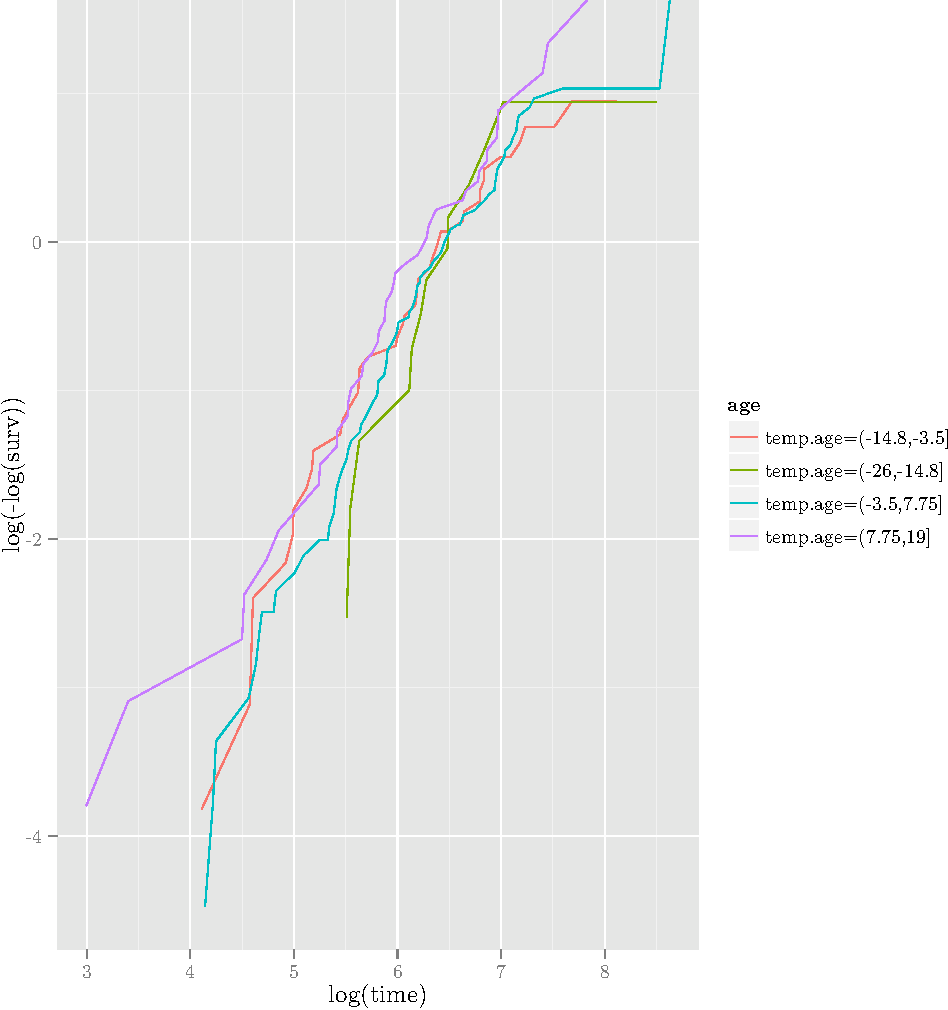
\includegraphics[width=\maxwidth]{figure/05-eda-ph-check-full-age-1} 

}



\end{knitrout}
Not perfect but it'll do.


\subsection{Outliers: full model}
Look at deviance residuals, both marginally and stratified by major subgroups.
\begin{knitrout}
\definecolor{shadecolor}{rgb}{0.969, 0.969, 0.969}\color{fgcolor}\begin{kframe}
\begin{alltt}
\hlkwd{plot}\hlstd{(}\hlkwd{resid}\hlstd{(fit.cph,} \hlkwc{type} \hlstd{=} \hlstr{"deviance"}\hlstd{))}
\hlkwd{abline}\hlstd{(}\hlkwc{h} \hlstd{=} \hlkwd{c}\hlstd{(}\hlopt{-}\hlnum{2.5}\hlstd{,} \hlnum{2.5}\hlstd{))}
\end{alltt}
\end{kframe}

{\centering 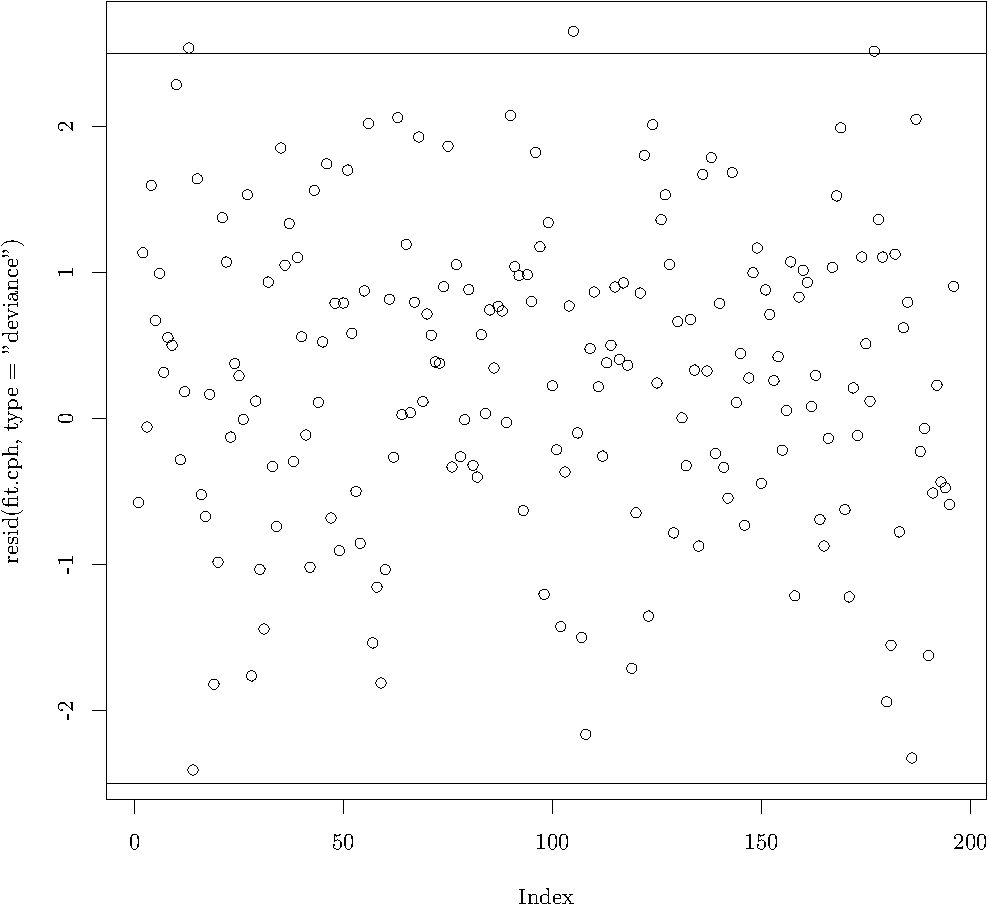
\includegraphics[width=\maxwidth]{figure/05-eda-outliers-full-1} 

}


\begin{kframe}\begin{alltt}
\hlstd{temp.ord} \hlkwb{=} \hlkwd{order}\hlstd{(data}\hlopt{$}\hlstd{SexM, data}\hlopt{$}\hlstd{A2, data}\hlopt{$}\hlstd{A4)}
\hlstd{temp.resid} \hlkwb{=} \hlkwd{resid}\hlstd{(fit.cph,} \hlkwc{type} \hlstd{=} \hlstr{"deviance"}\hlstd{)[temp.ord]}
\hlstd{temp.col} \hlkwb{=} \hlstd{(}\hlnum{4}\hlopt{*}\hlstd{data}\hlopt{$}\hlstd{SexM} \hlopt{+} \hlnum{2}\hlopt{*}\hlstd{data}\hlopt{$}\hlstd{A2} \hlopt{+} \hlstd{data}\hlopt{$}\hlstd{A4} \hlopt{+} \hlnum{1}\hlstd{)[temp.ord]}
\hlkwd{plot}\hlstd{(temp.resid,} \hlkwc{col} \hlstd{= temp.col,} \hlkwc{pch} \hlstd{=} \hlnum{16}\hlstd{)}
\hlkwd{abline}\hlstd{(}\hlkwc{h} \hlstd{=} \hlkwd{c}\hlstd{(}\hlopt{-}\hlnum{2.5}\hlstd{,} \hlnum{2.5}\hlstd{))}
\end{alltt}
\end{kframe}

{\centering 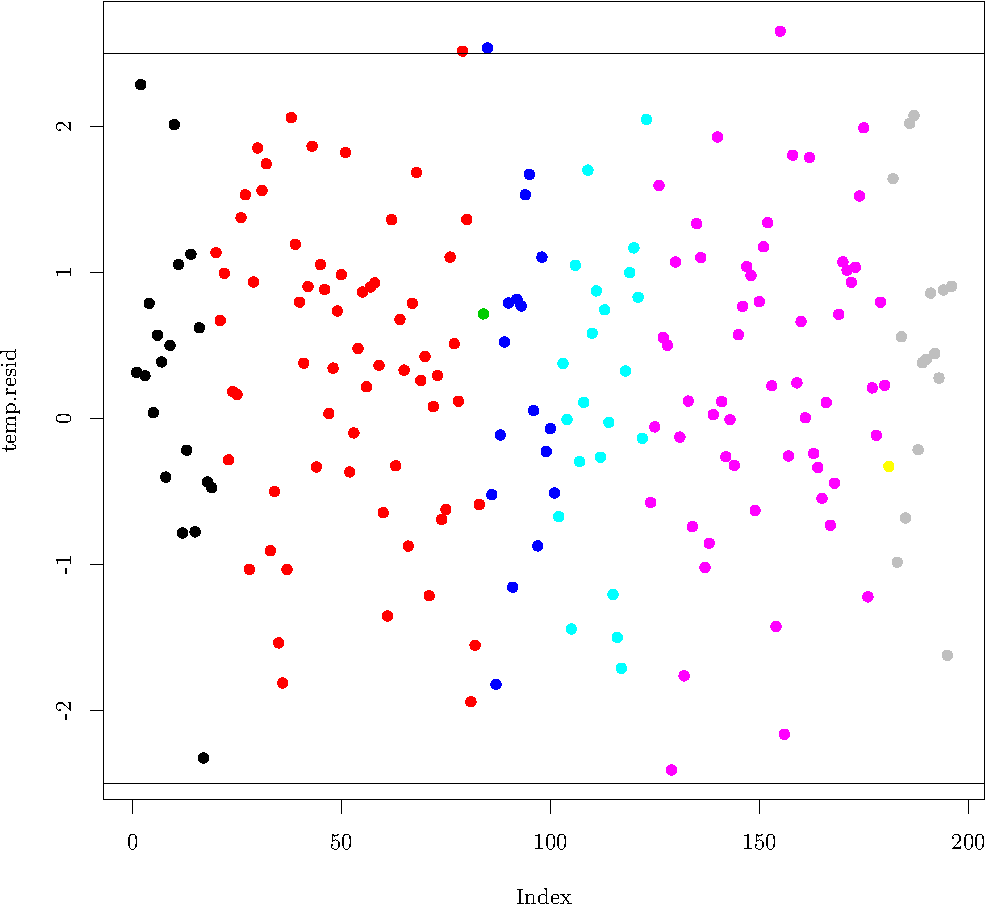
\includegraphics[width=\maxwidth]{figure/05-eda-outliers-full-2} 

}


\begin{kframe}\begin{alltt}
\hlkwd{boxplot}\hlstd{(}\hlkwd{resid}\hlstd{(fit.cph,} \hlkwc{type} \hlstd{=} \hlstr{"deviance"}\hlstd{)} \hlopt{~} \hlstd{data}\hlopt{$}\hlstd{SexM} \hlopt{+} \hlstd{data}\hlopt{$}\hlstd{A2} \hlopt{+} \hlstd{data}\hlopt{$}\hlstd{A4,} \hlkwc{varwidth} \hlstd{=} \hlnum{TRUE}\hlstd{)}
\hlkwd{abline}\hlstd{(}\hlkwc{h} \hlstd{=} \hlnum{0}\hlstd{)}
\end{alltt}
\end{kframe}

{\centering 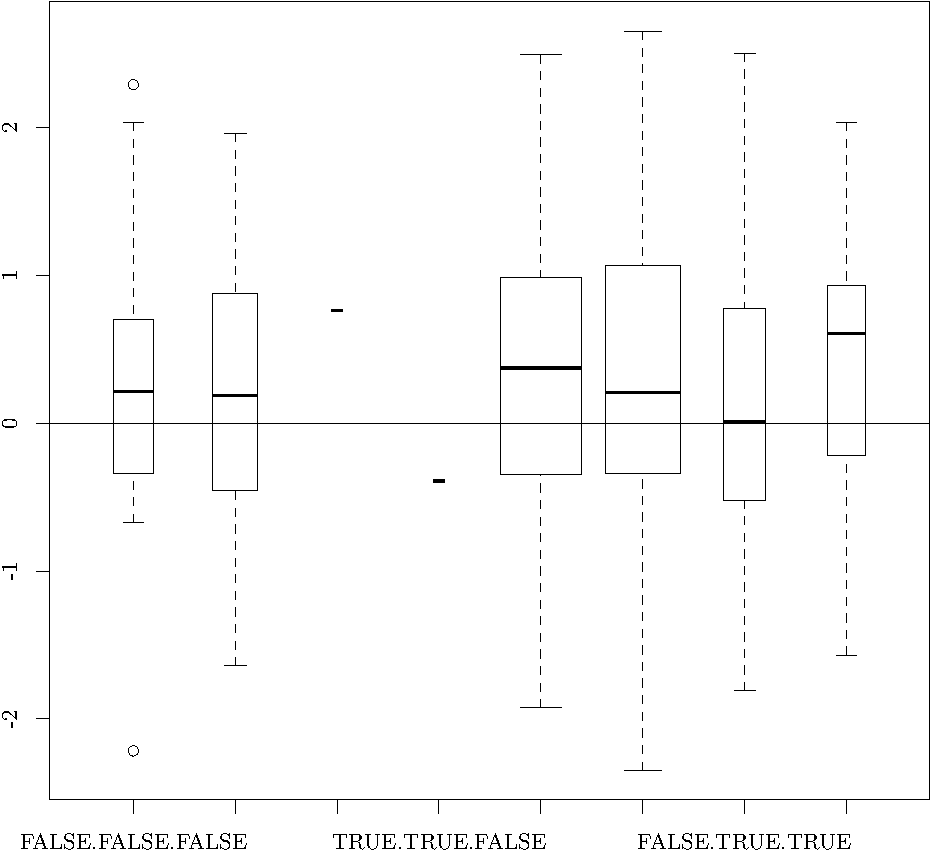
\includegraphics[width=\maxwidth]{figure/05-eda-outliers-full-3} 

}


\begin{kframe}\begin{alltt}
\hlkwd{boxplot}\hlstd{(}\hlkwd{resid}\hlstd{(fit.cph,} \hlkwc{type} \hlstd{=} \hlstr{"martingale"}\hlstd{)} \hlopt{~} \hlstd{data}\hlopt{$}\hlstd{SexM} \hlopt{+} \hlstd{data}\hlopt{$}\hlstd{A2} \hlopt{+} \hlstd{data}\hlopt{$}\hlstd{A4,} \hlkwc{varwidth} \hlstd{=} \hlnum{TRUE}\hlstd{)}
\hlkwd{abline}\hlstd{(}\hlkwc{h} \hlstd{=} \hlnum{0}\hlstd{)}
\end{alltt}
\end{kframe}

{\centering 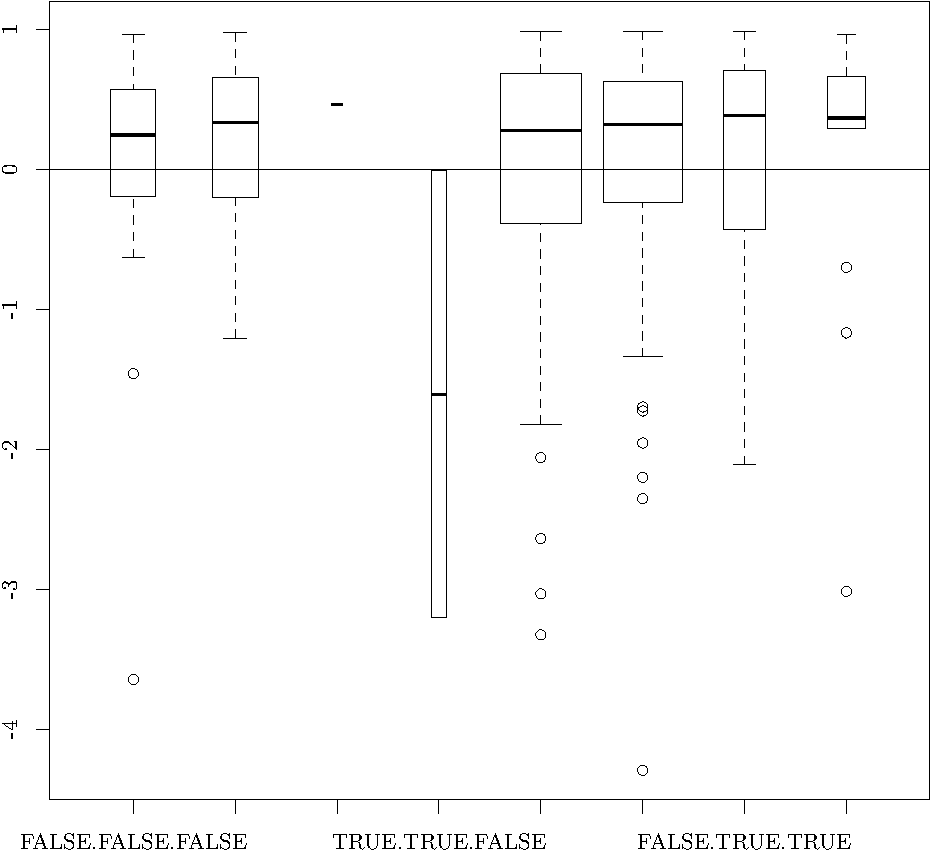
\includegraphics[width=\maxwidth]{figure/05-eda-outliers-full-4} 

}



\end{knitrout}

Use DFBETAS to examine influence.
\begin{knitrout}
\definecolor{shadecolor}{rgb}{0.969, 0.969, 0.969}\color{fgcolor}\begin{kframe}
\begin{alltt}
\hlstd{temp} \hlkwb{=} \hlkwd{resid}\hlstd{(fit.cph,} \hlkwc{type} \hlstd{=} \hlstr{"dfbetas"}\hlstd{)}
\hlkwd{colnames}\hlstd{(temp)} \hlkwb{=} \hlkwd{names}\hlstd{(fit.cph}\hlopt{$}\hlstd{coefficients)}
\hlstd{temp} \hlkwb{=} \hlkwd{melt}\hlstd{(temp)}
\hlkwd{colnames}\hlstd{(temp)} \hlkwb{=} \hlkwd{c}\hlstd{(}\hlstr{"Patient"}\hlstd{,} \hlstr{"Coefficient"}\hlstd{,} \hlstr{"dfbetas"}\hlstd{)}
\hlstd{temp}\hlopt{$}\hlstd{Patient} \hlkwb{=} \hlkwd{gsub}\hlstd{(}\hlstr{"NSWPCN_"}\hlstd{,} \hlstr{""}\hlstd{, temp}\hlopt{$}\hlstd{Patient)}
\hlkwd{ggplot}\hlstd{(temp,} \hlkwd{aes}\hlstd{(}\hlkwc{y} \hlstd{= dfbetas,} \hlkwc{x} \hlstd{= Patient,} \hlkwc{col} \hlstd{= Coefficient))} \hlopt{+} \hlkwd{geom_point}\hlstd{()}
\end{alltt}
\end{kframe}

{\centering 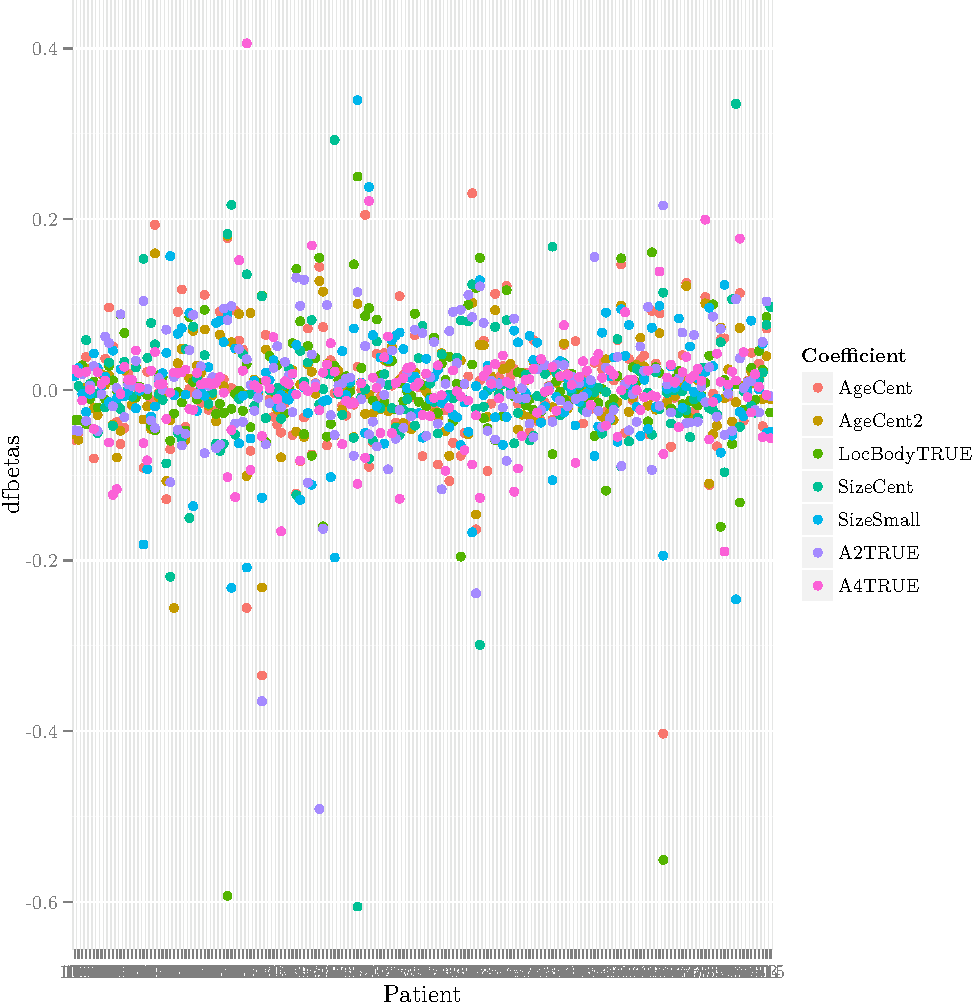
\includegraphics[width=\maxwidth]{figure/05-eda-dfbetas-full-1} 

}



\end{knitrout}
There is quite a number of rather influential observations.  These could do with some checking, but first collapse down the model -- there's little point doing dfbeta fucking about based on coefficients that will never get fit in the end anyway.


\subsection{EDA: Variable selection}
\begin{knitrout}
\definecolor{shadecolor}{rgb}{0.969, 0.969, 0.969}\color{fgcolor}\begin{kframe}
\begin{alltt}
\hlstd{nobs.coxph} \hlkwb{<<-} \hlkwa{function}\hlstd{(}\hlkwc{obj}\hlstd{,} \hlkwc{...}\hlstd{)} \hlkwd{sum}\hlstd{(obj}\hlopt{$}\hlstd{y[,}\hlnum{2}\hlstd{])}
\hlcom{# Note: Exhaustive search at level 2 is only feasible for at most 5 variables}
\hlcom{#fit.cph.as = glmulti(Surv(Time, DSD) ~ strata(SexM) + AgeCent + AgeCent2 + LocBody + SizeCent + SizeSmall + A2 + A4, data = data, marginality = TRUE, method = "h", fitfunction = "coxph", crit = "bic", level = 2)}
\hlkwd{set.seed}\hlstd{(}\hlnum{20150110}\hlstd{)}
\hlstd{fit.cph.as} \hlkwb{=} \hlkwd{glmulti}\hlstd{(}\hlkwd{Surv}\hlstd{(Time, DSD)} \hlopt{~} \hlkwd{strata}\hlstd{(SexM)} \hlopt{+} \hlstd{AgeCent} \hlopt{+} \hlstd{AgeCent2} \hlopt{+} \hlstd{LocBody} \hlopt{+} \hlstd{SizeCent} \hlopt{+} \hlstd{SizeSmall} \hlopt{+} \hlstd{A2} \hlopt{+} \hlstd{A4,} \hlkwc{data} \hlstd{= data,} \hlkwc{marginality} \hlstd{=} \hlnum{TRUE}\hlstd{,} \hlkwc{method} \hlstd{=} \hlstr{"g"}\hlstd{,} \hlkwc{fitfunction} \hlstd{=} \hlstr{"coxph"}\hlstd{,} \hlkwc{crit} \hlstd{=} \hlstr{"bic"}\hlstd{,} \hlkwc{level} \hlstd{=} \hlnum{2}\hlstd{,} \hlkwc{plotty} \hlstd{=} \hlnum{FALSE}\hlstd{,} \hlkwc{report} \hlstd{=} \hlnum{FALSE}\hlstd{)}
\end{alltt}
\begin{verbatim}
## TASK: Genetic algorithm in the candidate set.
## Initialization...
## Algorithm started...
\end{verbatim}


{\ttfamily\noindent\color{warningcolor}{\#\# Warning in fitter(X, Y, strats, offset, init, control, weights = weights, : Loglik converged before variable\ \ 9 ; beta may be infinite.}}

{\ttfamily\noindent\color{warningcolor}{\#\# Warning in fitter(X, Y, strats, offset, init, control, weights = weights, : Loglik converged before variable\ \ 12 ; beta may be infinite.}}

{\ttfamily\noindent\color{warningcolor}{\#\# Warning in fitter(X, Y, strats, offset, init, control, weights = weights, : Loglik converged before variable\ \ 12 ; beta may be infinite.}}

{\ttfamily\noindent\color{warningcolor}{\#\# Warning in fitter(X, Y, strats, offset, init, control, weights = weights, : Loglik converged before variable\ \ 21 ; beta may be infinite.}}\begin{verbatim}
## Improvements in best and average IC have bebingo en below the specified goals.
## Algorithm is declared to have converged.
## Completed.
\end{verbatim}
\begin{alltt}
\hlcom{# fit.cph.as}
\hlcom{# After 830 generations:}
\hlcom{# Best model: Surv(Time,DSD)~1+strata(SexM)+SizeCent+A2+A4}
\hlcom{# Crit= 1367.16344569113}
\hlcom{# Mean crit= 1401.37248769175}
\hlcom{# Improvements in best and average IC have bebingo en below the specified goals.}
\hlcom{# Algorithm is declared to have converged.}
\hlcom{# Completed.}
\hlkwd{rm}\hlstd{(nobs.coxph)}
\end{alltt}
\end{kframe}
\end{knitrout}

Also run BIC stepwise, because we can.
\begin{knitrout}
\definecolor{shadecolor}{rgb}{0.969, 0.969, 0.969}\color{fgcolor}\begin{kframe}
\begin{alltt}
\hlkwd{stepAIC}\hlstd{(fit.cph,} \hlkwc{k} \hlstd{=} \hlkwd{log}\hlstd{(}\hlkwd{nrow}\hlstd{(data)))}
\end{alltt}
\begin{verbatim}
## Start:  AIC=1269
## Surv(Time, DSD) ~ strata(SexM) + AgeCent + AgeCent2 + LocBody + 
##     SizeCent + SizeSmall + A2 + A4
## 
##             Df  AIC
## - AgeCent    1 1264
## - LocBody    1 1264
## - SizeSmall  1 1264
## - AgeCent2   1 1266
## - SizeCent   1 1267
## <none>         1269
## - A2         1 1272
## - A4         1 1272
## 
## Step:  AIC=1264
## Surv(Time, DSD) ~ strata(SexM) + AgeCent2 + LocBody + SizeCent + 
##     SizeSmall + A2 + A4
## 
##             Df  AIC
## - LocBody    1 1259
## - SizeSmall  1 1259
## - AgeCent2   1 1261
## - SizeCent   1 1262
## <none>         1264
## - A2         1 1266
## - A4         1 1267
## 
## Step:  AIC=1259
## Surv(Time, DSD) ~ strata(SexM) + AgeCent2 + SizeCent + SizeSmall + 
##     A2 + A4
## 
##             Df  AIC
## - SizeSmall  1 1254
## - AgeCent2   1 1256
## - SizeCent   1 1257
## <none>         1259
## - A2         1 1261
## - A4         1 1262
## 
## Step:  AIC=1254
## Surv(Time, DSD) ~ strata(SexM) + AgeCent2 + SizeCent + A2 + A4
## 
##            Df  AIC
## - AgeCent2  1 1252
## - SizeCent  1 1253
## <none>        1254
## - A2        1 1257
## - A4        1 1257
## 
## Step:  AIC=1252
## Surv(Time, DSD) ~ strata(SexM) + SizeCent + A2 + A4
## 
##            Df  AIC
## - SizeCent  1 1250
## <none>        1252
## - A4        1 1253
## - A2        1 1254
## 
## Step:  AIC=1250
## Surv(Time, DSD) ~ strata(SexM) + A2 + A4
## 
##        Df  AIC
## <none>    1250
## - A4    1 1254
## - A2    1 1254
## Call:
## coxph(formula = Surv(Time, DSD) ~ strata(SexM) + A2 + A4, data = data)
## 
## 
##         coef exp(coef) se(coef)    z      p
## A2TRUE 0.630      1.88    0.201 3.14 0.0017
## A4TRUE 0.556      1.74    0.203 2.74 0.0061
## 
## Likelihood ratio test=19.8  on 2 df, p=4.97e-05  n= 183, number of events= 175
\end{verbatim}
\end{kframe}
\end{knitrout}
Consensus, excellent.


\subsection{PH assumption: reduced model}
\begin{knitrout}
\definecolor{shadecolor}{rgb}{0.969, 0.969, 0.969}\color{fgcolor}\begin{kframe}
\begin{alltt}
\hlstd{fit.cph} \hlkwb{=} \hlkwd{coxph}\hlstd{(}\hlkwd{Surv}\hlstd{(Time, DSD)} \hlopt{~} \hlkwd{strata}\hlstd{(SexM)} \hlopt{+} \hlstd{SizeCent} \hlopt{+} \hlstd{A2} \hlopt{+} \hlstd{A4,} \hlkwc{data} \hlstd{= data)}
\hlkwd{cox.zph}\hlstd{(fit.cph)}
\end{alltt}
\begin{verbatim}
##              rho  chisq     p
## SizeCent -0.0905 1.6290 0.202
## A2TRUE    0.0230 0.0922 0.761
## A4TRUE   -0.0815 1.1103 0.292
## GLOBAL        NA 3.1175 0.374
\end{verbatim}
\begin{alltt}
\hlkwd{plot}\hlstd{(}\hlkwd{cox.zph}\hlstd{(fit.cph))}
\end{alltt}
\end{kframe}

{\centering 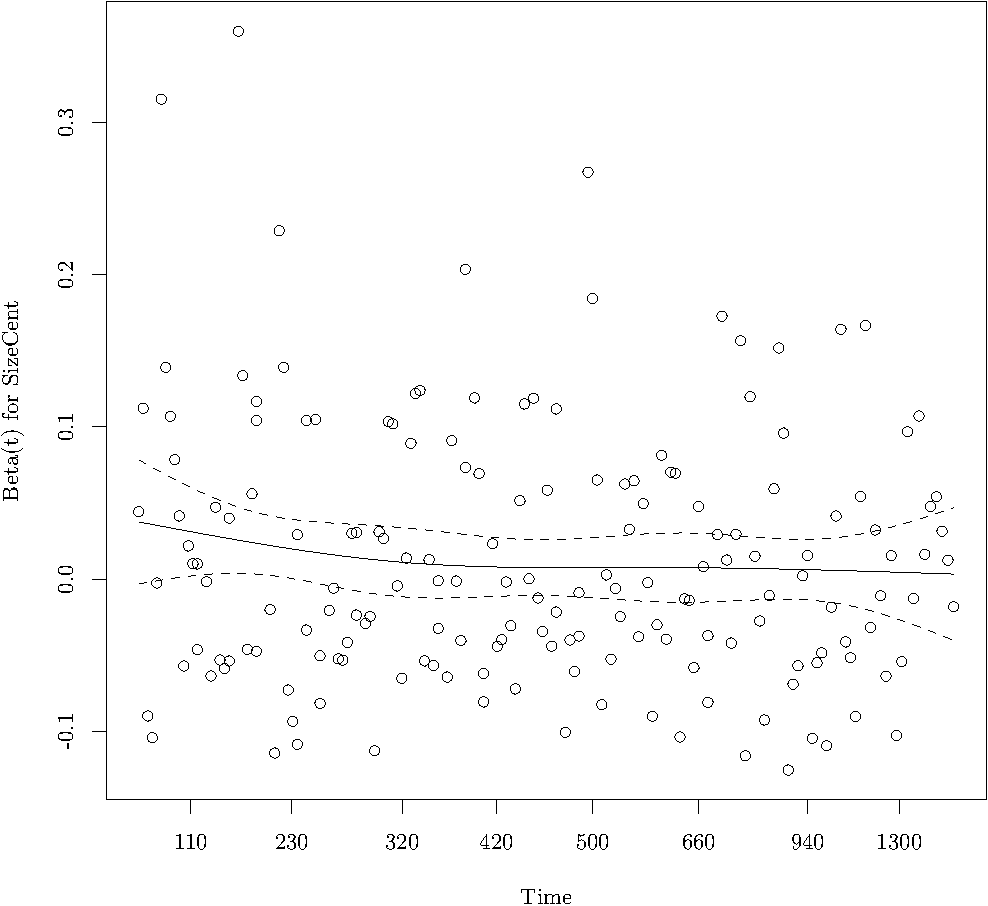
\includegraphics[width=\maxwidth]{figure/05-eda-ph-check-reduced-1} 

}




{\centering 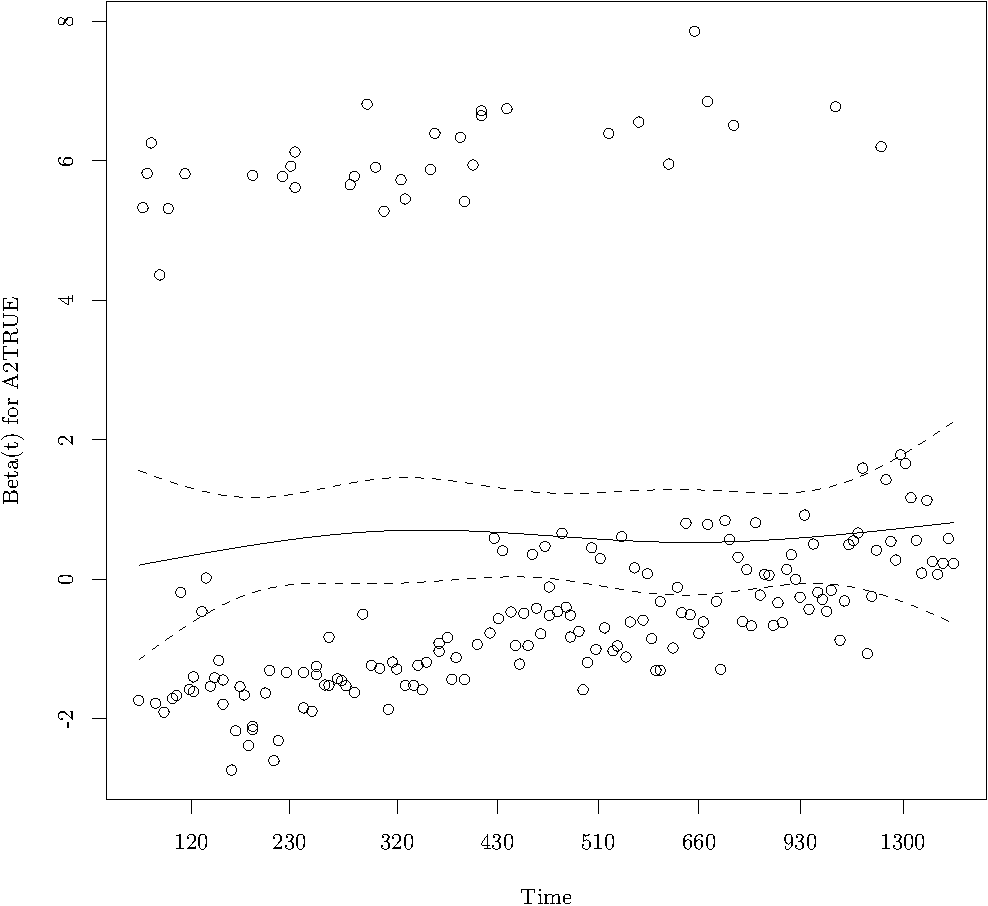
\includegraphics[width=\maxwidth]{figure/05-eda-ph-check-reduced-2} 

}




{\centering 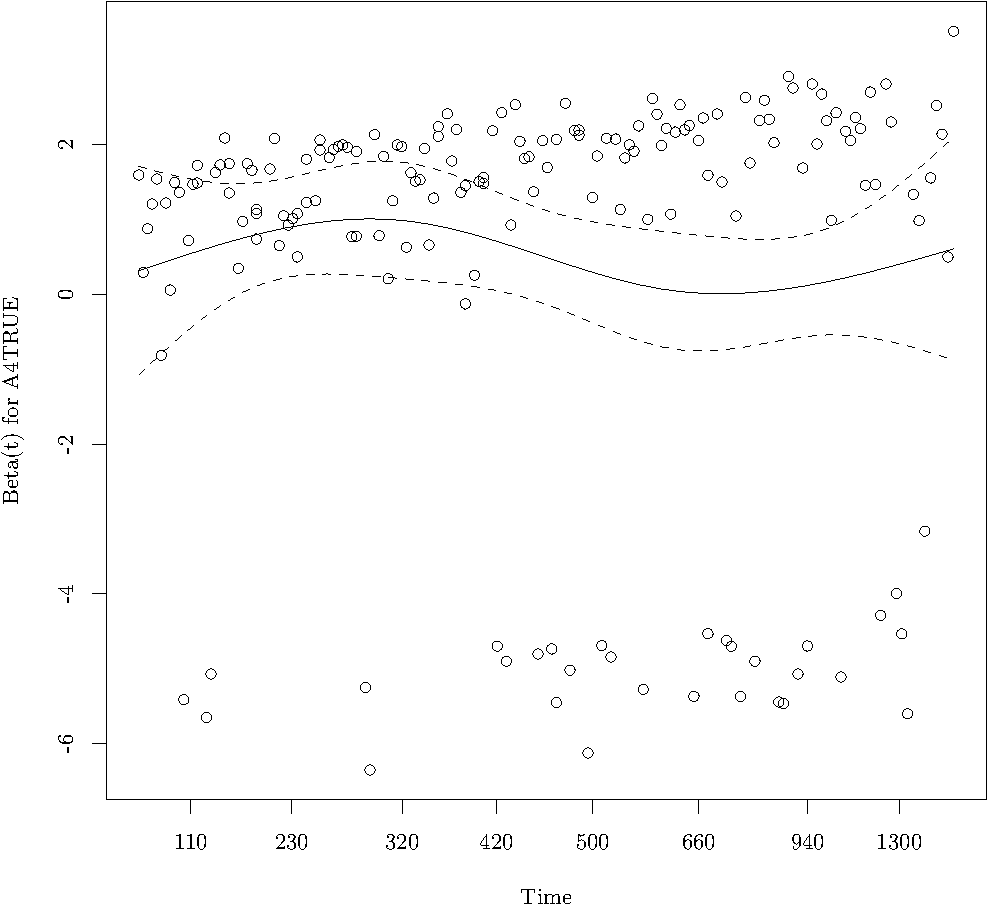
\includegraphics[width=\maxwidth]{figure/05-eda-ph-check-reduced-3} 

}



\end{knitrout}

\subsection{Outliers: reduced model}
\begin{knitrout}
\definecolor{shadecolor}{rgb}{0.969, 0.969, 0.969}\color{fgcolor}\begin{kframe}
\begin{alltt}
\hlkwd{plot}\hlstd{(}\hlkwd{resid}\hlstd{(fit.cph,} \hlkwc{type} \hlstd{=} \hlstr{"deviance"}\hlstd{))}
\end{alltt}
\end{kframe}

{\centering 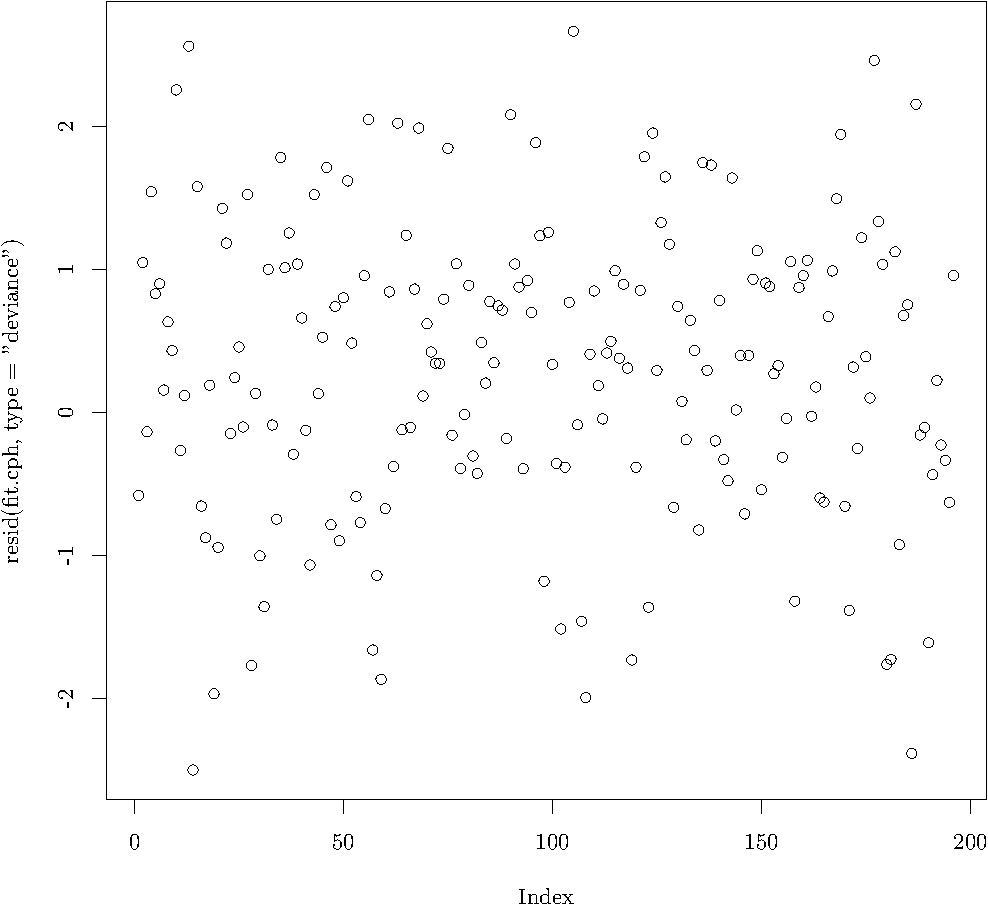
\includegraphics[width=\maxwidth]{figure/05-eda-outliers-reduced-1} 

}



\end{knitrout}

Now generate the restricted fit and examine the DFBETAS on the reduced model.

\begin{knitrout}
\definecolor{shadecolor}{rgb}{0.969, 0.969, 0.969}\color{fgcolor}\begin{kframe}
\begin{alltt}
\hlstd{temp} \hlkwb{=} \hlkwd{resid}\hlstd{(fit.cph,} \hlkwc{type} \hlstd{=} \hlstr{"dfbetas"}\hlstd{)}
\hlkwd{colnames}\hlstd{(temp)} \hlkwb{=} \hlkwd{names}\hlstd{(fit.cph}\hlopt{$}\hlstd{coefficients)}
\hlstd{temp} \hlkwb{=} \hlkwd{melt}\hlstd{(temp)}
\hlkwd{colnames}\hlstd{(temp)} \hlkwb{=} \hlkwd{c}\hlstd{(}\hlstr{"Patient"}\hlstd{,} \hlstr{"Coefficient"}\hlstd{,} \hlstr{"dfbetas"}\hlstd{)}
\hlstd{temp}\hlopt{$}\hlstd{Patient} \hlkwb{=} \hlkwd{gsub}\hlstd{(}\hlstr{"NSWPCN_"}\hlstd{,} \hlstr{""}\hlstd{, temp}\hlopt{$}\hlstd{Patient)}
\hlnum{2}\hlopt{/}\hlkwd{sqrt}\hlstd{(}\hlkwd{nrow}\hlstd{(data))}              \hlcom{# The classic threshold for concern is 2/sqrt(n).}
\end{alltt}
\begin{verbatim}
## [1] 0.1478
\end{verbatim}
\begin{alltt}
\hlkwd{ggplot}\hlstd{(temp,} \hlkwd{aes}\hlstd{(}\hlkwc{y} \hlstd{=} \hlkwd{abs}\hlstd{(dfbetas),} \hlkwc{x} \hlstd{= Patient,} \hlkwc{col} \hlstd{= Coefficient))} \hlopt{+} \hlkwd{geom_point}\hlstd{()} \hlopt{+} \hlkwd{geom_hline}\hlstd{(}\hlkwc{yintercept} \hlstd{=} \hlnum{2}\hlopt{/}\hlkwd{sqrt}\hlstd{(}\hlkwd{nrow}\hlstd{(data)))}
\end{alltt}
\end{kframe}

{\centering 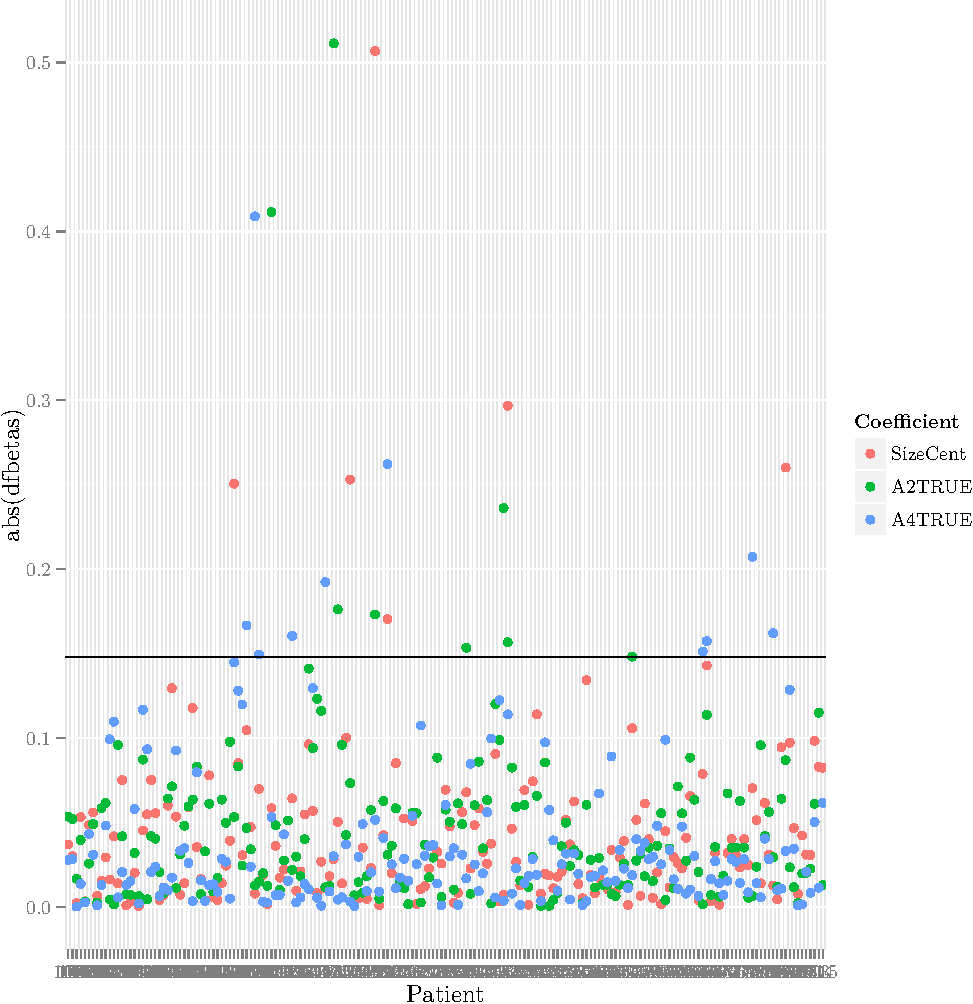
\includegraphics[width=\maxwidth]{figure/05-eda-dfbetas-reduced-1} 

}


\begin{kframe}\begin{alltt}
\hlkwd{sort}\hlstd{(}\hlkwd{apply}\hlstd{(}\hlkwd{abs}\hlstd{(}\hlkwd{resid}\hlstd{(fit.cph,} \hlkwc{type} \hlstd{=} \hlstr{"dfbetas"}\hlstd{)),} \hlnum{1}\hlstd{, max),} \hlkwc{decreasing} \hlstd{=} \hlnum{TRUE}\hlstd{)}
\end{alltt}
\begin{verbatim}
##  NSWPCN_144  NSWPCN_183 NSWPCN_1212 NSWPCN_1195  NSWPCN_318  NSWPCN_195 
##    0.511340    0.506815    0.411412    0.408937    0.296728    0.262110 
##  NSWPCN_799  NSWPCN_154 NSWPCN_1182  NSWPCN_317  NSWPCN_777  NSWPCN_142 
##    0.260153    0.253014    0.250597    0.236114    0.207351    0.192280 
##  NSWPCN_145 NSWPCN_1188  NSWPCN_795  NSWPCN_125  NSWPCN_655  NSWPCN_296 
##    0.176188    0.166665    0.162051    0.160416    0.157420    0.153478 
##  NSWPCN_654 NSWPCN_1196  NSWPCN_374  NSWPCN_131  NSWPCN_354  NSWPCN_133 
##    0.151246    0.149449    0.148152    0.141058    0.134170    0.129507 
## NSWPCN_1155  NSWPCN_802 NSWPCN_1186  NSWPCN_135  NSWPCN_316  NSWPCN_315 
##    0.129471    0.128471    0.128036    0.123203    0.122328    0.120121 
## NSWPCN_1187 NSWPCN_1167 NSWPCN_1143  NSWPCN_138  NSWPCN_814  NSWPCN_333 
##    0.119838    0.117793    0.116717    0.116009    0.114995    0.114018 
## NSWPCN_1072  NSWPCN_269  NSWPCN_152  NSWPCN_312 NSWPCN_1071  NSWPCN_636 
##    0.109648    0.107374    0.100089    0.099732    0.099250    0.099010 
##  NSWPCN_813 NSWPCN_1179  NSWPCN_335 NSWPCN_1453 NSWPCN_1082  NSWPCN_789 
##    0.098347    0.097750    0.097415    0.095938    0.095841    0.095735 
##  NSWPCN_798 NSWPCN_1145 NSWPCN_1157  NSWPCN_364  NSWPCN_647  NSWPCN_276 
##    0.094433    0.093340    0.092592    0.089047    0.088390    0.088343 
##  NSWPCN_305  NSWPCN_200  NSWPCN_303 NSWPCN_1168  NSWPCN_322  NSWPCN_815 
##    0.085945    0.085147    0.084780    0.082972    0.082445    0.082391 
## NSWPCN_1172 NSWPCN_1146 NSWPCN_1088  NSWPCN_331  NSWPCN_640  NSWPCN_281 
##    0.077888    0.075122    0.075085    0.074289    0.071269    0.069418 
##  NSWPCN_326  NSWPCN_664  NSWPCN_360 NSWPCN_1153 NSWPCN_1177  NSWPCN_651 
##    0.069060    0.067170    0.067089    0.064155    0.063501    0.063455 
##  NSWPCN_310  NSWPCN_194  NSWPCN_769  NSWPCN_351 NSWPCN_1029  NSWPCN_790 
##    0.063192    0.062687    0.062634    0.062402    0.061529    0.061523 
##  NSWPCN_284  NSWPCN_377  NSWPCN_304 NSWPCN_1165  NSWPCN_324 NSWPCN_1028 
##    0.061268    0.061213    0.060116    0.059436    0.059216    0.058363 
## NSWPCN_1139  NSWPCN_336  NSWPCN_182  NSWPCN_794  NSWPCN_294 NSWPCN_1023 
##    0.057912    0.057377    0.057341    0.056127    0.056116    0.055877 
##  NSWPCN_257  NSWPCN_445 NSWPCN_1147  NSWPCN_268  NSWPCN_643   NSWPCN_13 
##    0.055813    0.055469    0.055464    0.055426    0.055403    0.054730 
##   NSWPCN_10 NSWPCN_1019   NSWPCN_24 NSWPCN_1016  NSWPCN_347  NSWPCN_375 
##    0.053392    0.053156    0.052313    0.052050    0.051517    0.051489 
##  NSWPCN_781 NSWPCN_1227  NSWPCN_282 NSWPCN_1178  NSWPCN_164 NSWPCN_1022 
##    0.051333    0.051115    0.050311    0.049749    0.048995    0.048464 
## NSWPCN_1213 NSWPCN_1160    NSWPCN_4 NSWPCN_1190  NSWPCN_804 NSWPCN_1219 
##    0.048263    0.048105    0.048021    0.047256    0.046638    0.042923 
##  NSWPCN_807  NSWPCN_646  NSWPCN_666  NSWPCN_381  NSWPCN_770  NSWPCN_341 
##    0.042281    0.040889    0.040225    0.040068    0.040056    0.039362 
##  NSWPCN_370  NSWPCN_350  NSWPCN_270  NSWPCN_273   NSWPCN_20  NSWPCN_272 
##    0.038992    0.037026    0.036778    0.036591    0.036201    0.035952 
##  NSWPCN_346  NSWPCN_657    NSWPCN_7  NSWPCN_283  NSWPCN_309  NSWPCN_637 
##    0.035888    0.035464    0.035127    0.034719    0.034677    0.034559 
##  NSWPCN_369 NSWPCN_1158  NSWPCN_376 NSWPCN_1171  NSWPCN_810  NSWPCN_352 
##    0.033701    0.033208    0.033132    0.032882    0.030954    0.030734 
##  NSWPCN_811  NSWPCN_126  NSWPCN_161  NSWPCN_384  NSWPCN_638  NSWPCN_358 
##    0.030726    0.029736    0.029730    0.029667    0.029548    0.027843 
##  NSWPCN_280  NSWPCN_775  NSWPCN_362  NSWPCN_128  NSWPCN_653 NSWPCN_1150 
##    0.025663    0.024846    0.021612    0.020969    0.020569    0.020533 
## NSWPCN_1207  NSWPCN_662   NSWPCN_36  NSWPCN_330  NSWPCN_143  NSWPCN_166 
##    0.019948    0.018477    0.018340    0.018191    0.018187    0.018185 
##  NSWPCN_345 NSWPCN_1215   NSWPCN_21 NSWPCN_1176 NSWPCN_1018  NSWPCN_656 
##    0.017812    0.017340    0.017265    0.017131    0.016678    0.016425 
## NSWPCN_1170  NSWPCN_325  NSWPCN_256  NSWPCN_366 NSWPCN_1136  NSWPCN_363 
##    0.016398    0.015592    0.015547    0.015304    0.015192    0.014593 
##  NSWPCN_658 NSWPCN_1175 NSWPCN_1091  NSWPCN_373 NSWPCN_1211  NSWPCN_797 
##    0.014004    0.013425    0.013036    0.012972    0.012450    0.011917 
## NSWPCN_1152  NSWPCN_190  NSWPCN_334  NSWPCN_806  NSWPCN_157 NSWPCN_1027 
##    0.011502    0.009024    0.007702    0.007660    0.006790    0.006582 
## NSWPCN_1140  NSWPCN_353 NSWPCN_1020 
##    0.006373    0.005084    0.003220
\end{verbatim}
\begin{alltt}
\hlkwd{sum}\hlstd{(}\hlkwd{apply}\hlstd{(}\hlkwd{abs}\hlstd{(}\hlkwd{resid}\hlstd{(fit.cph,} \hlkwc{type} \hlstd{=} \hlstr{"dfbetas"}\hlstd{)),} \hlnum{1}\hlstd{, max)} \hlopt{>} \hlnum{2}\hlopt{/}\hlkwd{sqrt}\hlstd{(}\hlkwd{nrow}\hlstd{(data)))}
\end{alltt}
\begin{verbatim}
## [1] 21
\end{verbatim}
\end{kframe}
\end{knitrout}

\subsection{Summary of EDA}
\begin{enumerate}
\item On the basis of pre-operative assessability and data availability, variables were filtered down to Sex, AgeCent, LocBody, SizeCent, A2, A4.
\item Functional forms for the continuous variates AgeCent and SizeCent indicated a possible slight quadratic effect on AgeCent, and a knee on SizeCent.  These were modelled by incorporating additional terms.
\item Analysis of a full model fit (with additional nonlinear terms included) indicated violation of PH for gender.  This was dealt with by stratification.  A slight PH violation by age was deemed unimportant. 
\item Variable selection by BIC (both stepwise and genetic all-subset) settled on a final model of Surv(Time,DSD) $\sim$ 1 + strata(SexM) + SizeCent + A2 + A4.  This model was refit by coxph. 
\item PH was verified on the final model.  Deviance residuals showed no egregious outliers. dfBetaS indicated a number of influential observations, which require checking.
\end{enumerate}

\section{Final fits}
\begin{knitrout}
\definecolor{shadecolor}{rgb}{0.969, 0.969, 0.969}\color{fgcolor}\begin{kframe}
\begin{alltt}
\hlstd{fit.cph} \hlkwb{=} \hlkwd{coxph}\hlstd{(}\hlkwd{Surv}\hlstd{(Time, DSD)} \hlopt{~} \hlkwd{strata}\hlstd{(SexM)} \hlopt{+} \hlstd{SizeCent} \hlopt{+} \hlstd{A2} \hlopt{+} \hlstd{A4,} \hlkwc{data} \hlstd{= data)}
\end{alltt}
\end{kframe}
\end{knitrout}

\begin{knitrout}
\definecolor{shadecolor}{rgb}{0.969, 0.969, 0.969}\color{fgcolor}\begin{kframe}
\begin{alltt}
\hlkwd{set.seed}\hlstd{(}\hlnum{20150111}\hlstd{)}
\hlstd{fit.rsf} \hlkwb{=} \hlkwd{rfsrc}\hlstd{(}\hlkwd{Surv}\hlstd{(Time, DSD)} \hlopt{~} \hlstd{SexM} \hlopt{+} \hlstd{AgeCent} \hlopt{+} \hlstd{LocBody} \hlopt{+} \hlstd{SizeCent} \hlopt{+} \hlstd{A2} \hlopt{+} \hlstd{A4,} \hlkwc{data} \hlstd{= data,} \hlkwc{mtry} \hlstd{=} \hlnum{1}\hlstd{,} \hlkwc{splitrule} \hlstd{=} \hlstr{"logrankscore"}\hlstd{,} \hlkwc{nsplit} \hlstd{=} \hlnum{2}\hlstd{,} \hlkwc{ntree} \hlstd{=} \hlnum{1000}\hlstd{)}
\end{alltt}
\end{kframe}
\end{knitrout}

\begin{knitrout}
\definecolor{shadecolor}{rgb}{0.969, 0.969, 0.969}\color{fgcolor}\begin{kframe}
\begin{alltt}
\hlstd{fit.gg} \hlkwb{=} \hlkwd{flexsurvreg}\hlstd{(}\hlkwd{Surv}\hlstd{(Time, DSD)} \hlopt{~} \hlstd{SexM} \hlopt{+} \hlstd{SizeCent} \hlopt{+} \hlstd{A2} \hlopt{+} \hlstd{A4,}
        \hlkwc{anc} \hlstd{=} \hlkwd{list}\hlstd{(}
                \hlkwc{sigma} \hlstd{=} \hlopt{~} \hlstd{SexM,}
                \hlkwc{Q} \hlstd{=} \hlopt{~} \hlstd{SexM),}
        \hlkwc{data} \hlstd{= data,} \hlkwc{dist} \hlstd{=} \hlstr{"gengamma"}\hlstd{)}

\hlstd{fit.gf} \hlkwb{=} \hlkwd{flexsurvreg}\hlstd{(}\hlkwd{Surv}\hlstd{(Time, DSD)} \hlopt{~} \hlstd{SexM} \hlopt{+} \hlstd{SizeCent} \hlopt{+} \hlstd{A2} \hlopt{+} \hlstd{A4,}
        \hlkwc{anc} \hlstd{=} \hlkwd{list}\hlstd{(}
                \hlkwc{sigma} \hlstd{=} \hlopt{~} \hlstd{SexM,}
                \hlkwc{Q} \hlstd{=} \hlopt{~} \hlstd{SexM,}
                \hlkwc{P} \hlstd{=} \hlopt{~} \hlstd{SexM),}
        \hlkwc{data} \hlstd{= data,} \hlkwc{dist} \hlstd{=} \hlstr{"genf"}\hlstd{)}

\hlstd{fit.gg}\hlopt{$}\hlstd{loglik}
\end{alltt}
\begin{verbatim}
## [1] -1263
\end{verbatim}
\begin{alltt}
\hlstd{fit.gf}\hlopt{$}\hlstd{loglik}
\end{alltt}
\begin{verbatim}
## [1] -1262
\end{verbatim}
\begin{alltt}
\hlkwd{pchisq}\hlstd{(}\hlnum{2}\hlopt{*}\hlstd{(fit.gf}\hlopt{$}\hlstd{loglik} \hlopt{-} \hlstd{fit.gg}\hlopt{$}\hlstd{loglik),} \hlnum{2}\hlstd{,} \hlkwc{lower.tail} \hlstd{=} \hlnum{FALSE}\hlstd{)}
\end{alltt}
\begin{verbatim}
## [1] 0.3625
\end{verbatim}
\begin{alltt}
\hlkwd{AIC}\hlstd{(fit.gg)}
\end{alltt}
\begin{verbatim}
## [1] 2545
\end{verbatim}
\begin{alltt}
\hlkwd{AIC}\hlstd{(fit.gf)}
\end{alltt}
\begin{verbatim}
## [1] 2547
\end{verbatim}
\begin{alltt}
\hlkwd{BIC}\hlstd{(fit.gg)}
\end{alltt}
\begin{verbatim}
## [1] 2574
\end{verbatim}
\begin{alltt}
\hlkwd{BIC}\hlstd{(fit.gf)}
\end{alltt}
\begin{verbatim}
## [1] 2582
\end{verbatim}
\begin{alltt}
\hlstd{fit.gg}
\end{alltt}
\begin{verbatim}
## 
## Call:
## flexsurvreg(formula = Surv(Time, DSD) ~ SexM + SizeCent + A2 +     A4, anc = list(sigma = ~SexM, Q = ~SexM), data = data, dist = "gengamma")
## 
## Estimates: 
##                  data mean  est       L95%      U95%      se      
## mu                     NA    6.44681   6.07286   6.82076   0.19079
## sigma                  NA    0.80245   0.69416   0.92763   0.05935
## Q                      NA    0.06179  -0.51053   0.63411   0.29201
## SexMTRUE          0.47541    0.38255   0.03482   0.73028   0.17742
## SizeCent          3.18579   -0.00953  -0.01742  -0.00164   0.00403
## A2TRUE            0.18033   -0.38859  -0.66061  -0.11657   0.13879
## A4TRUE            0.80328   -0.36208  -0.63874  -0.08542   0.14116
## sigma(SexMTRUE)   0.47541   -0.25308  -0.49389  -0.01227   0.12287
## Q(SexMTRUE)       0.47541    0.78916   0.03792   1.54039   0.38329
##                  exp(est)  L95%      U95%    
## mu                     NA        NA        NA
## sigma                  NA        NA        NA
## Q                      NA        NA        NA
## SexMTRUE          1.46602   1.03543   2.07567
## SizeCent          0.99052   0.98274   0.99837
## A2TRUE            0.67801   0.51653   0.88997
## A4TRUE            0.69623   0.52796   0.91812
## sigma(SexMTRUE)   0.77640   0.61025   0.98781
## Q(SexMTRUE)       2.20154   1.03865   4.66643
## 
## N = 183,  Events: 175,  Censored: 8
## Total time at risk: 106023
## Log-likelihood = -1263, df = 9
## AIC = 2545
\end{verbatim}
\end{kframe}
\end{knitrout}

\section{Fit assessment}
Plot fit stratified by sex, separate curves for A2, A4 status, at median (approx.) Size.
\begin{knitrout}
\definecolor{shadecolor}{rgb}{0.969, 0.969, 0.969}\color{fgcolor}\begin{kframe}
\begin{alltt}
\hlstd{temp.grid} \hlkwb{=} \hlkwd{expand.grid}\hlstd{(}\hlkwc{A4} \hlstd{=} \hlkwd{c}\hlstd{(}\hlnum{FALSE}\hlstd{,} \hlnum{TRUE}\hlstd{),} \hlkwc{A2} \hlstd{=} \hlkwd{c}\hlstd{(}\hlnum{FALSE}\hlstd{,} \hlnum{TRUE}\hlstd{),} \hlkwc{SexM} \hlstd{=} \hlkwd{c}\hlstd{(}\hlnum{FALSE}\hlstd{,} \hlnum{TRUE}\hlstd{),} \hlkwc{SizeCent} \hlstd{=} \hlnum{0}\hlstd{)}
\hlstd{temp.grid}\hlopt{$}\hlstd{ID} \hlkwb{=} \hlkwd{sprintf}\hlstd{(}\hlstr{"SexM=%s, A2=% -5s, A4=% -5s"}\hlstd{, temp.grid}\hlopt{$}\hlstd{SexM, temp.grid}\hlopt{$}\hlstd{A2, temp.grid}\hlopt{$}\hlstd{A4)}
\hlstd{temp.preds} \hlkwb{=} \hlkwd{summary}\hlstd{(fit.gg,} \hlkwc{newdata} \hlstd{= temp.grid,} \hlkwc{type} \hlstd{=} \hlstr{"survival"}\hlstd{,} \hlkwc{t} \hlstd{=} \hlkwd{seq}\hlstd{(}\hlnum{0}\hlstd{,} \hlnum{365}\hlopt{*}\hlnum{5}\hlstd{,} \hlnum{30}\hlstd{))}
\hlstd{temp.preds2} \hlkwb{=} \hlkwd{do.call}\hlstd{(rbind, temp.preds)}
\hlstd{temp.preds2}\hlopt{$}\hlstd{group} \hlkwb{=} \hlkwd{rep}\hlstd{(}\hlkwd{gsub}\hlstd{(}\hlstr{".*ID="}\hlstd{,} \hlstr{""}\hlstd{,} \hlkwd{names}\hlstd{(temp.preds)),} \hlkwc{each} \hlstd{=} \hlkwd{nrow}\hlstd{(temp.preds[[}\hlnum{1}\hlstd{]]))}
\hlstd{temp.preds.cox} \hlkwb{=} \hlkwd{survfit}\hlstd{(fit.cph,} \hlkwc{newdata} \hlstd{= temp.grid)}

\hlstd{temp.survfit} \hlkwb{=} \hlkwd{survfit}\hlstd{(}\hlkwd{Surv}\hlstd{(Time, DSD)} \hlopt{~} \hlstd{SexM} \hlopt{+} \hlstd{A2} \hlopt{+} \hlstd{A4, data)}
\hlstd{temp.data} \hlkwb{=} \hlkwd{data.frame}\hlstd{(}\hlkwc{time} \hlstd{= temp.survfit}\hlopt{$}\hlstd{time,} \hlkwc{surv} \hlstd{= temp.survfit}\hlopt{$}\hlstd{surv,} \hlkwc{upper} \hlstd{= temp.survfit}\hlopt{$}\hlstd{lower,} \hlkwc{lower} \hlstd{= temp.survfit}\hlopt{$}\hlstd{upper,} \hlkwc{group} \hlstd{=} \hlkwd{rep}\hlstd{(}\hlkwd{names}\hlstd{(temp.survfit}\hlopt{$}\hlstd{strata), temp.survfit}\hlopt{$}\hlstd{strata),} \hlkwc{model} \hlstd{=} \hlstr{"KM"}\hlstd{)}
\hlstd{temp.data} \hlkwb{=} \hlkwd{rbind}\hlstd{(temp.data,} \hlkwd{data.frame}\hlstd{(}\hlkwc{time} \hlstd{= temp.preds2}\hlopt{$}\hlstd{time,} \hlkwc{surv} \hlstd{= temp.preds2}\hlopt{$}\hlstd{est,} \hlkwc{upper} \hlstd{= temp.preds2}\hlopt{$}\hlstd{ucl,} \hlkwc{lower} \hlstd{= temp.preds2}\hlopt{$}\hlstd{lcl,} \hlkwc{group} \hlstd{= temp.preds2}\hlopt{$}\hlstd{group,} \hlkwc{model} \hlstd{=} \hlstr{"GG"}\hlstd{))}
\hlstd{temp.data} \hlkwb{=} \hlkwd{rbind}\hlstd{(temp.data,} \hlkwd{data.frame}\hlstd{(}\hlkwc{time} \hlstd{= temp.preds.cox}\hlopt{$}\hlstd{time,} \hlkwc{surv} \hlstd{= temp.preds.cox}\hlopt{$}\hlstd{surv,} \hlkwc{upper} \hlstd{= temp.preds.cox}\hlopt{$}\hlstd{upper,} \hlkwc{lower} \hlstd{= temp.preds.cox}\hlopt{$}\hlstd{lower,} \hlkwc{group} \hlstd{=} \hlkwd{rep}\hlstd{(temp.grid}\hlopt{$}\hlstd{ID, temp.preds.cox}\hlopt{$}\hlstd{strata),} \hlkwc{model} \hlstd{=} \hlstr{"CPH"}\hlstd{))}

\hlstd{temp.data}\hlopt{$}\hlstd{Sex} \hlkwb{=} \hlkwd{c}\hlstd{(}\hlstr{"Male"}\hlstd{,} \hlstr{"Female"}\hlstd{)[}\hlkwd{grepl}\hlstd{(}\hlstr{"SexM=FALSE"}\hlstd{, temp.data}\hlopt{$}\hlstd{group)}\hlopt{+}\hlnum{1}\hlstd{]}
\hlstd{temp.data}\hlopt{$}\hlstd{A2} \hlkwb{=} \hlkwd{c}\hlstd{(}\hlstr{"A2-"}\hlstd{,} \hlstr{"A2+"}\hlstd{)[}\hlkwd{grepl}\hlstd{(}\hlstr{"A2=TRUE"}\hlstd{, temp.data}\hlopt{$}\hlstd{group)}\hlopt{+}\hlnum{1}\hlstd{]}
\hlstd{temp.data}\hlopt{$}\hlstd{A4} \hlkwb{=} \hlkwd{c}\hlstd{(}\hlstr{"A4-"}\hlstd{,} \hlstr{"A4+"}\hlstd{)[}\hlkwd{grepl}\hlstd{(}\hlstr{"A4=TRUE"}\hlstd{, temp.data}\hlopt{$}\hlstd{group)}\hlopt{+}\hlnum{1}\hlstd{]}

\hlkwd{ggplot}\hlstd{(temp.data,} \hlkwd{aes}\hlstd{(}\hlkwc{x} \hlstd{=} \hlkwd{log}\hlstd{(time),} \hlkwc{y} \hlstd{=} \hlkwd{log}\hlstd{(}\hlopt{-}\hlkwd{log}\hlstd{(surv)),} \hlkwc{ymin} \hlstd{=} \hlkwd{log}\hlstd{(}\hlopt{-}\hlkwd{log}\hlstd{(lower)),} \hlkwc{ymax} \hlstd{=} \hlkwd{log}\hlstd{(}\hlopt{-}\hlkwd{log}\hlstd{(upper)),} \hlkwc{colour} \hlstd{= model,} \hlkwc{fill} \hlstd{= model))} \hlopt{+}
        \hlkwd{geom_ribbon}\hlstd{(}\hlkwc{alpha} \hlstd{=} \hlnum{0.25}\hlstd{,} \hlkwc{colour} \hlstd{=} \hlnum{NA}\hlstd{)} \hlopt{+}
        \hlkwd{geom_line}\hlstd{()} \hlopt{+}
        \hlkwd{xlim}\hlstd{(}\hlnum{4}\hlstd{,} \hlnum{7}\hlstd{)} \hlopt{+} \hlkwd{ylim}\hlstd{(}\hlopt{-}\hlnum{4}\hlstd{,} \hlnum{2}\hlstd{)} \hlopt{+}
        \hlkwd{facet_grid}\hlstd{(A2} \hlopt{~} \hlstd{A4} \hlopt{~} \hlstd{Sex)}
\end{alltt}


{\ttfamily\noindent\color{warningcolor}{\#\# Warning: Removed 46 rows containing missing values (geom\_path).}}

{\ttfamily\noindent\color{warningcolor}{\#\# Warning: Removed 39 rows containing missing values (geom\_path).}}

{\ttfamily\noindent\color{warningcolor}{\#\# Warning: Removed 48 rows containing missing values (geom\_path).}}

{\ttfamily\noindent\color{warningcolor}{\#\# Warning: Removed 43 rows containing missing values (geom\_path).}}

{\ttfamily\noindent\color{warningcolor}{\#\# Warning: Removed 39 rows containing missing values (geom\_path).}}

{\ttfamily\noindent\color{warningcolor}{\#\# Warning: Removed 36 rows containing missing values (geom\_path).}}

{\ttfamily\noindent\color{warningcolor}{\#\# Warning: Removed 40 rows containing missing values (geom\_path).}}

{\ttfamily\noindent\color{warningcolor}{\#\# Warning: Removed 37 rows containing missing values (geom\_path).}}\end{kframe}

{\centering 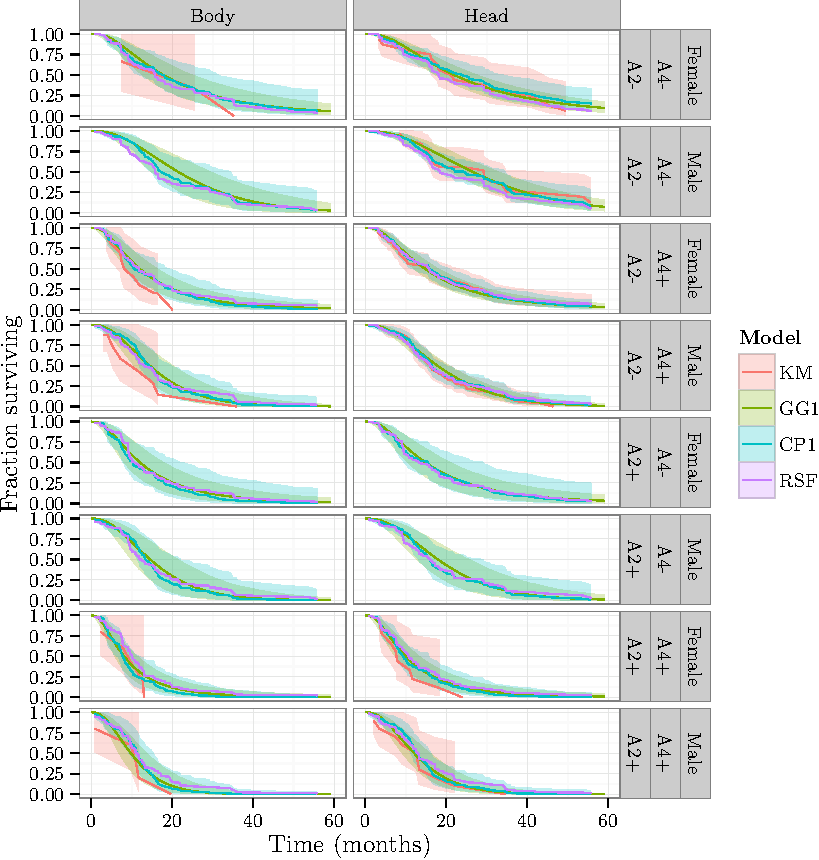
\includegraphics[width=\maxwidth]{figure/05-final-fit-assessment-1} 

}


\begin{kframe}\begin{alltt}
\hlkwd{ggplot}\hlstd{(temp.data,} \hlkwd{aes}\hlstd{(}\hlkwc{x} \hlstd{= time,} \hlkwc{y} \hlstd{= surv,} \hlkwc{ymin} \hlstd{= lower,} \hlkwc{ymax} \hlstd{= upper,} \hlkwc{colour} \hlstd{= model,} \hlkwc{fill} \hlstd{= model))} \hlopt{+}
        \hlkwd{geom_ribbon}\hlstd{(}\hlkwc{alpha} \hlstd{=} \hlnum{0.25}\hlstd{,} \hlkwc{colour} \hlstd{=} \hlnum{NA}\hlstd{)} \hlopt{+}
        \hlkwd{geom_line}\hlstd{()} \hlopt{+} \hlkwd{xlim}\hlstd{(}\hlnum{0}\hlstd{,} \hlnum{2000}\hlstd{)} \hlopt{+} \hlkwd{ylim}\hlstd{(}\hlnum{0}\hlstd{,} \hlnum{1}\hlstd{)} \hlopt{+}
        \hlkwd{facet_grid}\hlstd{(A2} \hlopt{~} \hlstd{A4} \hlopt{~} \hlstd{Sex)}
\end{alltt}


{\ttfamily\noindent\color{warningcolor}{\#\# Warning: Removed 3 rows containing missing values (geom\_path).}}

{\ttfamily\noindent\color{warningcolor}{\#\# Warning: Removed 3 rows containing missing values (geom\_path).}}

{\ttfamily\noindent\color{warningcolor}{\#\# Warning: Removed 2 rows containing missing values (geom\_path).}}

{\ttfamily\noindent\color{warningcolor}{\#\# Warning: Removed 2 rows containing missing values (geom\_path).}}\end{kframe}

{\centering 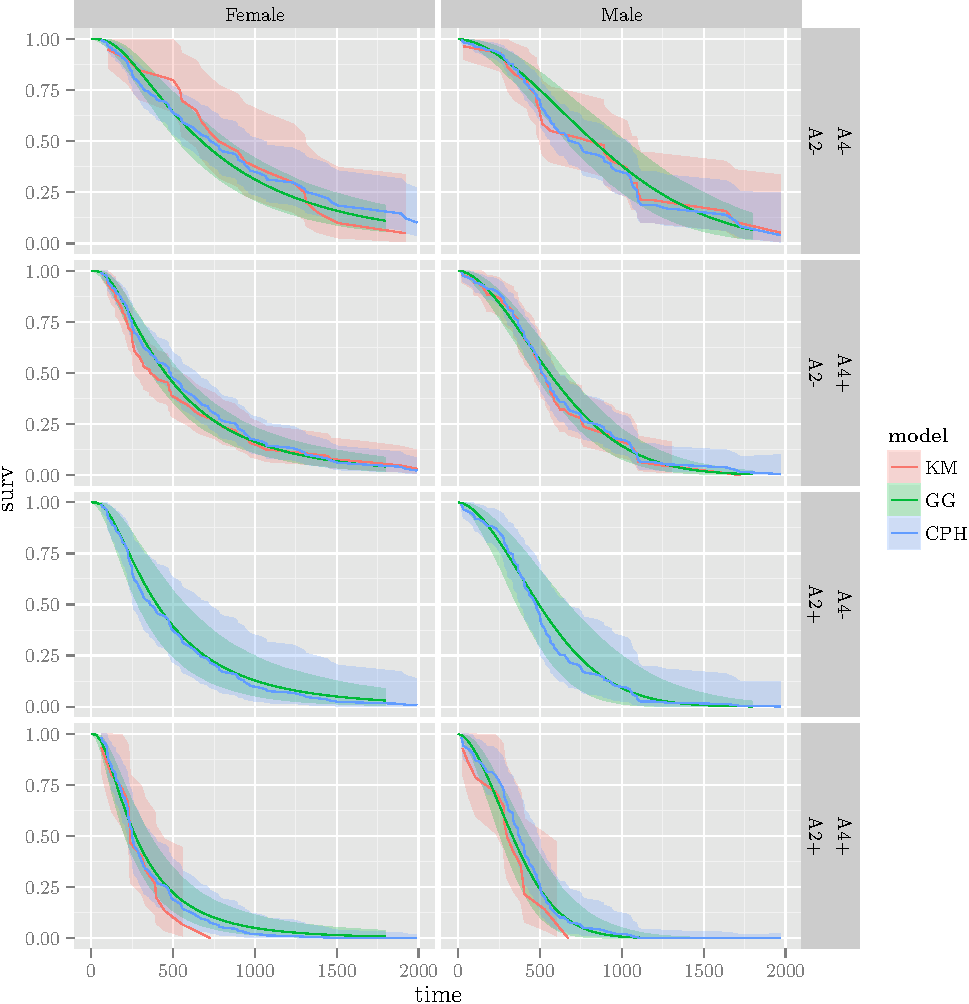
\includegraphics[width=\maxwidth]{figure/05-final-fit-assessment-2} 

}



\end{knitrout}

Some deviation though not significant.  Most concerning is the A2- A4- female group, survival of which is underestimated by the flexsurv model.  To approach this in a modelling sense would require interaction terms between Sex and A2, A4. Overfitting seems likely considering the very few data available for the A2+/A4- group.  Perhaps just add a single "DoubleNegFemale" term.
\begin{knitrout}
\definecolor{shadecolor}{rgb}{0.969, 0.969, 0.969}\color{fgcolor}\begin{kframe}
\begin{alltt}
\hlstd{fit.gg2} \hlkwb{=} \hlkwd{flexsurvreg}\hlstd{(}\hlkwd{Surv}\hlstd{(Time, DSD)} \hlopt{~} \hlstd{SexM} \hlopt{+} \hlstd{SizeCent} \hlopt{+} \hlstd{A2} \hlopt{+} \hlstd{A4} \hlopt{+} \hlkwd{I}\hlstd{(SexM} \hlopt{==} \hlnum{FALSE} \hlopt{&} \hlstd{A2} \hlopt{==} \hlnum{FALSE} \hlopt{&} \hlstd{A4} \hlopt{==} \hlnum{FALSE}\hlstd{),}
        \hlkwc{anc} \hlstd{=} \hlkwd{list}\hlstd{(}
                \hlkwc{sigma} \hlstd{=} \hlopt{~} \hlstd{SexM,}
                \hlkwc{Q} \hlstd{=} \hlopt{~} \hlstd{SexM),}
        \hlkwc{data} \hlstd{= data,} \hlkwc{dist} \hlstd{=} \hlstr{"gengamma"}\hlstd{)}

\hlstd{fit.gg2}
\end{alltt}
\begin{verbatim}
## 
## Call:
## flexsurvreg(formula = Surv(Time, DSD) ~ SexM + SizeCent + A2 +     A4 + I(SexM == FALSE & A2 == FALSE & A4 == FALSE), anc = list(sigma = ~SexM,     Q = ~SexM), data = data, dist = "gengamma")
## 
## Estimates: 
##                                                   data mean  est     
## mu                                                      NA    6.37090
## sigma                                                   NA    0.79990
## Q                                                       NA    0.09541
## SexMTRUE                                           0.47541    0.40816
## SizeCent                                           3.18579   -0.00941
## A2TRUE                                             0.18033   -0.38417
## A4TRUE                                             0.80328   -0.29393
## I(SexM == FALSE & A2 == FALSE & A4 == FALSE)TRUE   0.08197    0.19993
## sigma(SexMTRUE)                                    0.47541   -0.25570
## Q(SexMTRUE)                                        0.47541    0.76926
##                                                   L95%      U95%    
## mu                                                 5.95233   6.78948
## sigma                                              0.69156   0.92521
## Q                                                 -0.46926   0.66007
## SexMTRUE                                           0.05768   0.75863
## SizeCent                                          -0.01726  -0.00156
## A2TRUE                                            -0.65634  -0.11200
## A4TRUE                                            -0.62047   0.03260
## I(SexM == FALSE & A2 == FALSE & A4 == FALSE)TRUE  -0.35382   0.75369
## sigma(SexMTRUE)                                   -0.49656  -0.01485
## Q(SexMTRUE)                                        0.02665   1.51187
##                                                   se        exp(est)
## mu                                                 0.21356        NA
## sigma                                              0.05939        NA
## Q                                                  0.28810        NA
## SexMTRUE                                           0.17882   1.50404
## SizeCent                                           0.00401   0.99064
## A2TRUE                                             0.13886   0.68102
## A4TRUE                                             0.16660   0.74533
## I(SexM == FALSE & A2 == FALSE & A4 == FALSE)TRUE   0.28253   1.22132
## sigma(SexMTRUE)                                    0.12289   0.77437
## Q(SexMTRUE)                                        0.37889   2.15816
##                                                   L95%      U95%    
## mu                                                      NA        NA
## sigma                                                   NA        NA
## Q                                                       NA        NA
## SexMTRUE                                           1.05938   2.13535
## SizeCent                                           0.98289   0.99844
## A2TRUE                                             0.51875   0.89404
## A4TRUE                                             0.53769   1.03313
## I(SexM == FALSE & A2 == FALSE & A4 == FALSE)TRUE   0.70200   2.12482
## sigma(SexMTRUE)                                    0.60862   0.98526
## Q(SexMTRUE)                                        1.02701   4.53518
## 
## N = 183,  Events: 175,  Censored: 8
## Total time at risk: 106023
## Log-likelihood = -1263, df = 10
## AIC = 2546
\end{verbatim}
\begin{alltt}
\hlkwd{AIC}\hlstd{(fit.gg)}
\end{alltt}
\begin{verbatim}
## [1] 2545
\end{verbatim}
\begin{alltt}
\hlkwd{AIC}\hlstd{(fit.gg2)}
\end{alltt}
\begin{verbatim}
## [1] 2546
\end{verbatim}
\begin{alltt}
\hlkwd{AIC}\hlstd{(fit.gg)} \hlopt{-} \hlkwd{AIC}\hlstd{(fit.gg2)}
\end{alltt}
\begin{verbatim}
## [1] -1.505
\end{verbatim}
\begin{alltt}
\hlcom{# Equivocal on AIC.  BIC would favour gg then.}

\hlkwd{pchisq}\hlstd{(}\hlopt{-}\hlnum{2}\hlopt{*}\hlstd{(fit.gg}\hlopt{$}\hlstd{loglik} \hlopt{-} \hlstd{fit.gg2}\hlopt{$}\hlstd{loglik),} \hlnum{1}\hlstd{,} \hlkwc{lower.tail} \hlstd{=} \hlnum{FALSE}\hlstd{)}
\end{alltt}
\begin{verbatim}
## [1] 0.4815
\end{verbatim}
\begin{alltt}
\hlcom{# Not good evidence on LRT}
\end{alltt}
\end{kframe}
\end{knitrout}

See how it plots relative to the others.
\begin{knitrout}
\definecolor{shadecolor}{rgb}{0.969, 0.969, 0.969}\color{fgcolor}\begin{kframe}
\begin{alltt}
\hlstd{temp.preds} \hlkwb{=} \hlkwd{summary}\hlstd{(fit.gg2,} \hlkwc{newdata} \hlstd{= temp.grid,} \hlkwc{type} \hlstd{=} \hlstr{"survival"}\hlstd{,} \hlkwc{t} \hlstd{=} \hlkwd{seq}\hlstd{(}\hlnum{0}\hlstd{,} \hlnum{365}\hlopt{*}\hlnum{5}\hlstd{,} \hlnum{30}\hlstd{))}
\hlstd{temp.preds2} \hlkwb{=} \hlkwd{do.call}\hlstd{(rbind, temp.preds)}
\hlstd{temp.preds2}\hlopt{$}\hlstd{group} \hlkwb{=} \hlkwd{rep}\hlstd{(}\hlkwd{gsub}\hlstd{(}\hlstr{".*ID="}\hlstd{,} \hlstr{""}\hlstd{,} \hlkwd{names}\hlstd{(temp.preds)),} \hlkwc{each} \hlstd{=} \hlkwd{nrow}\hlstd{(temp.preds[[}\hlnum{1}\hlstd{]]))}
\hlstd{temp.data} \hlkwb{=} \hlkwd{rbind}\hlstd{(temp.data,} \hlkwd{data.frame}\hlstd{(}\hlkwc{time} \hlstd{= temp.preds2}\hlopt{$}\hlstd{time,} \hlkwc{surv} \hlstd{= temp.preds2}\hlopt{$}\hlstd{est,} \hlkwc{upper} \hlstd{= temp.preds2}\hlopt{$}\hlstd{ucl,} \hlkwc{lower} \hlstd{= temp.preds2}\hlopt{$}\hlstd{lcl,} \hlkwc{group} \hlstd{= temp.preds2}\hlopt{$}\hlstd{group,} \hlkwc{model} \hlstd{=} \hlstr{"GG2"}\hlstd{,} \hlkwc{Sex} \hlstd{=} \hlnum{NA}\hlstd{,} \hlkwc{A2} \hlstd{=} \hlnum{NA}\hlstd{,} \hlkwc{A4} \hlstd{=} \hlnum{NA}\hlstd{))}
\hlstd{temp.data}\hlopt{$}\hlstd{Sex} \hlkwb{=} \hlkwd{c}\hlstd{(}\hlstr{"Male"}\hlstd{,} \hlstr{"Female"}\hlstd{)[}\hlkwd{grepl}\hlstd{(}\hlstr{"SexM=FALSE"}\hlstd{, temp.data}\hlopt{$}\hlstd{group)}\hlopt{+}\hlnum{1}\hlstd{]}
\hlstd{temp.data}\hlopt{$}\hlstd{A2} \hlkwb{=} \hlkwd{c}\hlstd{(}\hlstr{"A2-"}\hlstd{,} \hlstr{"A2+"}\hlstd{)[}\hlkwd{grepl}\hlstd{(}\hlstr{"A2=TRUE"}\hlstd{, temp.data}\hlopt{$}\hlstd{group)}\hlopt{+}\hlnum{1}\hlstd{]}
\hlstd{temp.data}\hlopt{$}\hlstd{A4} \hlkwb{=} \hlkwd{c}\hlstd{(}\hlstr{"A4-"}\hlstd{,} \hlstr{"A4+"}\hlstd{)[}\hlkwd{grepl}\hlstd{(}\hlstr{"A4=TRUE"}\hlstd{, temp.data}\hlopt{$}\hlstd{group)}\hlopt{+}\hlnum{1}\hlstd{]}

\hlkwd{ggplot}\hlstd{(temp.data,} \hlkwd{aes}\hlstd{(}\hlkwc{x} \hlstd{=} \hlkwd{log}\hlstd{(time),} \hlkwc{y} \hlstd{=} \hlkwd{log}\hlstd{(}\hlopt{-}\hlkwd{log}\hlstd{(surv)),} \hlkwc{ymin} \hlstd{=} \hlkwd{log}\hlstd{(}\hlopt{-}\hlkwd{log}\hlstd{(lower)),} \hlkwc{ymax} \hlstd{=} \hlkwd{log}\hlstd{(}\hlopt{-}\hlkwd{log}\hlstd{(upper)),} \hlkwc{colour} \hlstd{= model,} \hlkwc{fill} \hlstd{= model))} \hlopt{+}
        \hlkwd{geom_ribbon}\hlstd{(}\hlkwc{alpha} \hlstd{=} \hlnum{0.25}\hlstd{,} \hlkwc{colour} \hlstd{=} \hlnum{NA}\hlstd{)} \hlopt{+}
        \hlkwd{geom_line}\hlstd{()} \hlopt{+}
        \hlkwd{xlim}\hlstd{(}\hlnum{4}\hlstd{,} \hlnum{7}\hlstd{)} \hlopt{+} \hlkwd{ylim}\hlstd{(}\hlopt{-}\hlnum{4}\hlstd{,} \hlnum{2}\hlstd{)} \hlopt{+}
        \hlkwd{facet_grid}\hlstd{(A2} \hlopt{~} \hlstd{A4} \hlopt{~} \hlstd{Sex)}
\end{alltt}


{\ttfamily\noindent\color{warningcolor}{\#\# Warning: Removed 71 rows containing missing values (geom\_path).}}

{\ttfamily\noindent\color{warningcolor}{\#\# Warning: Removed 64 rows containing missing values (geom\_path).}}

{\ttfamily\noindent\color{warningcolor}{\#\# Warning: Removed 73 rows containing missing values (geom\_path).}}

{\ttfamily\noindent\color{warningcolor}{\#\# Warning: Removed 68 rows containing missing values (geom\_path).}}

{\ttfamily\noindent\color{warningcolor}{\#\# Warning: Removed 64 rows containing missing values (geom\_path).}}

{\ttfamily\noindent\color{warningcolor}{\#\# Warning: Removed 61 rows containing missing values (geom\_path).}}

{\ttfamily\noindent\color{warningcolor}{\#\# Warning: Removed 65 rows containing missing values (geom\_path).}}

{\ttfamily\noindent\color{warningcolor}{\#\# Warning: Removed 62 rows containing missing values (geom\_path).}}\end{kframe}

{\centering 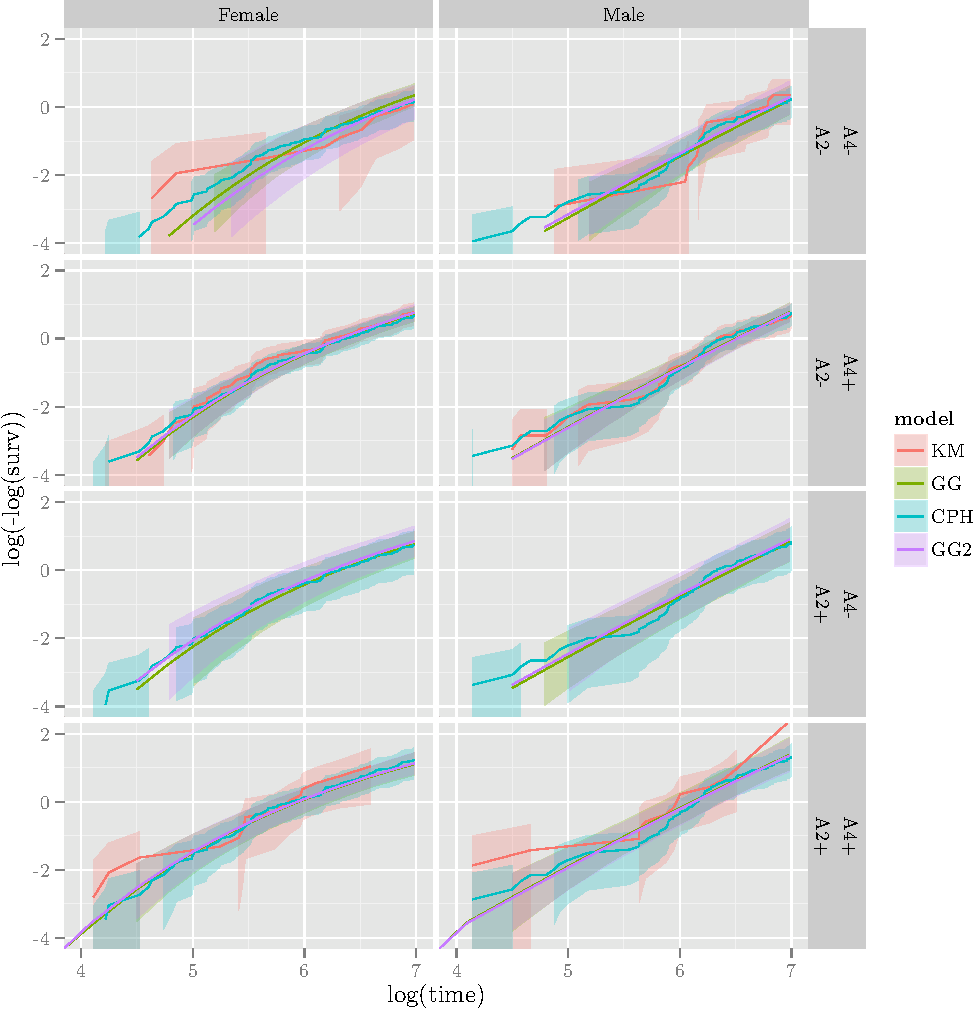
\includegraphics[width=\maxwidth]{figure/05-final-fit-assessment-2-1} 

}


\begin{kframe}\begin{alltt}
\hlkwd{ggplot}\hlstd{(temp.data,} \hlkwd{aes}\hlstd{(}\hlkwc{x} \hlstd{= time,} \hlkwc{y} \hlstd{= surv,} \hlkwc{ymin} \hlstd{= lower,} \hlkwc{ymax} \hlstd{= upper,} \hlkwc{colour} \hlstd{= model,} \hlkwc{fill} \hlstd{= model))} \hlopt{+}
        \hlkwd{geom_ribbon}\hlstd{(}\hlkwc{alpha} \hlstd{=} \hlnum{0.25}\hlstd{,} \hlkwc{colour} \hlstd{=} \hlnum{NA}\hlstd{)} \hlopt{+}
        \hlkwd{geom_line}\hlstd{()} \hlopt{+} \hlkwd{xlim}\hlstd{(}\hlnum{0}\hlstd{,} \hlnum{2000}\hlstd{)} \hlopt{+} \hlkwd{ylim}\hlstd{(}\hlnum{0}\hlstd{,} \hlnum{1}\hlstd{)} \hlopt{+}
        \hlkwd{facet_grid}\hlstd{(A2} \hlopt{~} \hlstd{A4} \hlopt{~} \hlstd{Sex)}
\end{alltt}


{\ttfamily\noindent\color{warningcolor}{\#\# Warning: Removed 3 rows containing missing values (geom\_path).}}

{\ttfamily\noindent\color{warningcolor}{\#\# Warning: Removed 3 rows containing missing values (geom\_path).}}

{\ttfamily\noindent\color{warningcolor}{\#\# Warning: Removed 2 rows containing missing values (geom\_path).}}

{\ttfamily\noindent\color{warningcolor}{\#\# Warning: Removed 2 rows containing missing values (geom\_path).}}\end{kframe}

{\centering 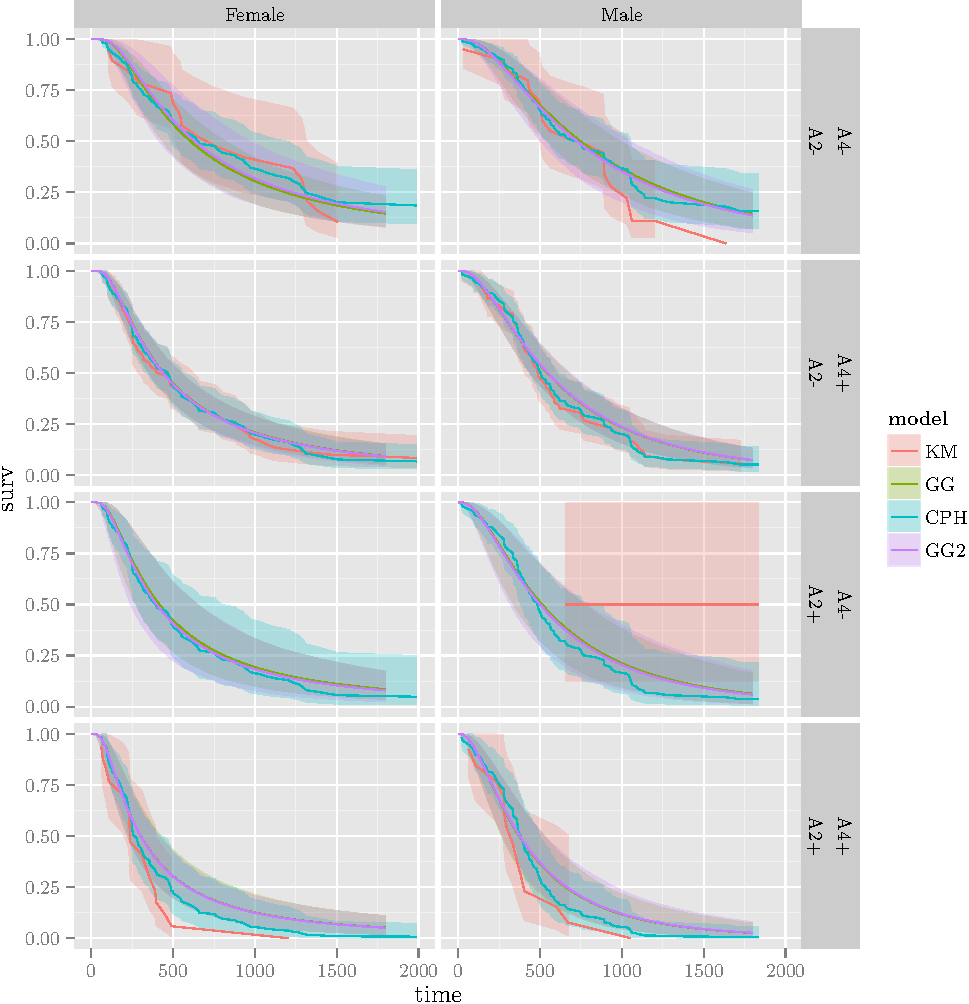
\includegraphics[width=\maxwidth]{figure/05-final-fit-assessment-2-2} 

}



\end{knitrout}

An alternative take, showing errors with the KMs only.
\begin{knitrout}
\definecolor{shadecolor}{rgb}{0.969, 0.969, 0.969}\color{fgcolor}\begin{kframe}
\begin{alltt}
\hlstd{temp.data}\hlopt{$}\hlstd{lower[temp.data}\hlopt{$}\hlstd{model} \hlopt{!=} \hlstr{"KM"}\hlstd{]} \hlkwb{=} \hlnum{NA}
\hlstd{temp.data}\hlopt{$}\hlstd{upper[temp.data}\hlopt{$}\hlstd{model} \hlopt{!=} \hlstr{"KM"}\hlstd{]} \hlkwb{=} \hlnum{NA}
\hlkwd{ggplot}\hlstd{(temp.data,} \hlkwd{aes}\hlstd{(}\hlkwc{x} \hlstd{=} \hlkwd{log}\hlstd{(time),} \hlkwc{y} \hlstd{=} \hlkwd{log}\hlstd{(}\hlopt{-}\hlkwd{log}\hlstd{(surv)),} \hlkwc{ymin} \hlstd{=} \hlkwd{log}\hlstd{(}\hlopt{-}\hlkwd{log}\hlstd{(lower)),} \hlkwc{ymax} \hlstd{=} \hlkwd{log}\hlstd{(}\hlopt{-}\hlkwd{log}\hlstd{(upper)),} \hlkwc{colour} \hlstd{= model,} \hlkwc{fill} \hlstd{= model))} \hlopt{+}
        \hlkwd{geom_ribbon}\hlstd{(}\hlkwc{alpha} \hlstd{=} \hlnum{0.25}\hlstd{,} \hlkwc{colour} \hlstd{=} \hlnum{NA}\hlstd{)} \hlopt{+}
        \hlkwd{geom_line}\hlstd{()} \hlopt{+}
        \hlkwd{xlim}\hlstd{(}\hlnum{4}\hlstd{,} \hlnum{7}\hlstd{)} \hlopt{+} \hlkwd{ylim}\hlstd{(}\hlopt{-}\hlnum{4}\hlstd{,} \hlnum{2}\hlstd{)} \hlopt{+}
        \hlkwd{facet_grid}\hlstd{(A2} \hlopt{~} \hlstd{A4} \hlopt{~} \hlstd{Sex)}
\end{alltt}


{\ttfamily\noindent\color{warningcolor}{\#\# Warning: Removed 71 rows containing missing values (geom\_path).}}

{\ttfamily\noindent\color{warningcolor}{\#\# Warning: Removed 64 rows containing missing values (geom\_path).}}

{\ttfamily\noindent\color{warningcolor}{\#\# Warning: Removed 73 rows containing missing values (geom\_path).}}

{\ttfamily\noindent\color{warningcolor}{\#\# Warning: Removed 68 rows containing missing values (geom\_path).}}

{\ttfamily\noindent\color{warningcolor}{\#\# Warning: Removed 64 rows containing missing values (geom\_path).}}

{\ttfamily\noindent\color{warningcolor}{\#\# Warning: Removed 61 rows containing missing values (geom\_path).}}

{\ttfamily\noindent\color{warningcolor}{\#\# Warning: Removed 65 rows containing missing values (geom\_path).}}

{\ttfamily\noindent\color{warningcolor}{\#\# Warning: Removed 62 rows containing missing values (geom\_path).}}\end{kframe}

{\centering 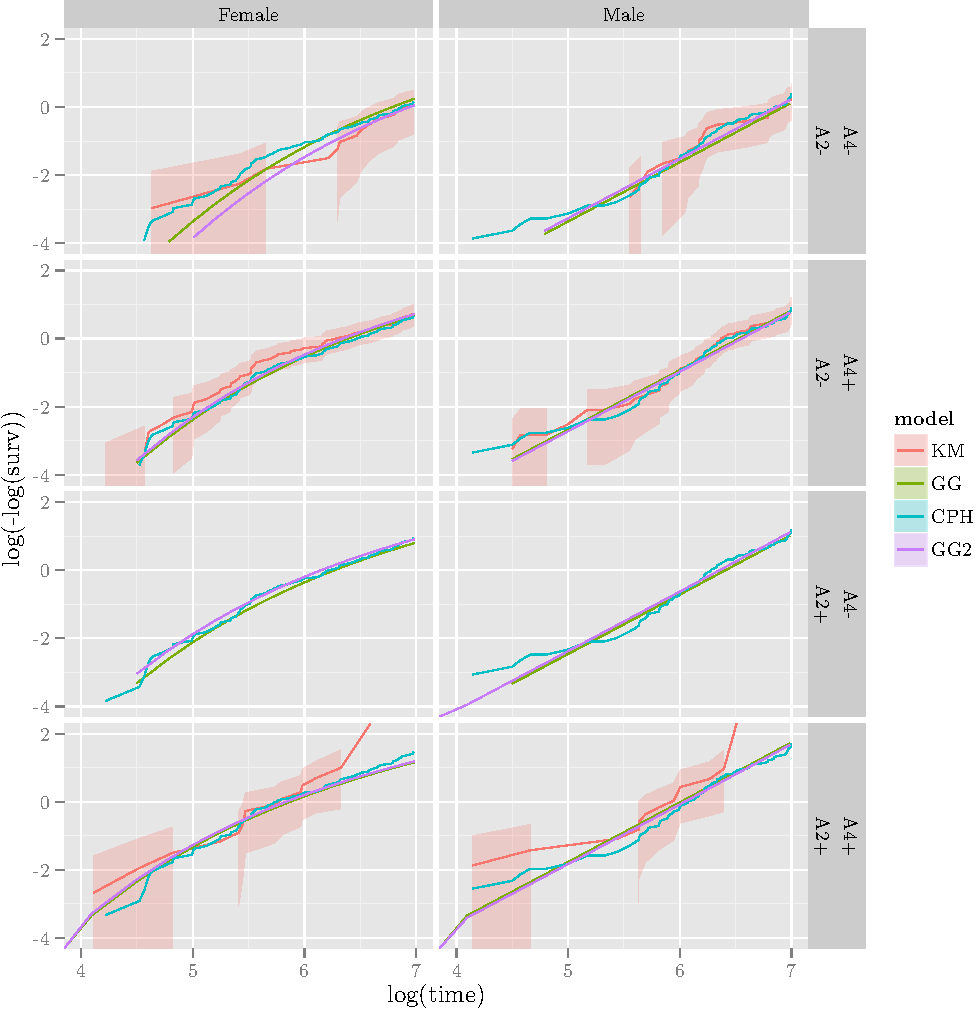
\includegraphics[width=\maxwidth]{figure/05-final-fit-assessment-3-1} 

}


\begin{kframe}\begin{alltt}
\hlkwd{ggplot}\hlstd{(temp.data,} \hlkwd{aes}\hlstd{(}\hlkwc{x} \hlstd{= time,} \hlkwc{y} \hlstd{= surv,} \hlkwc{ymin} \hlstd{= lower,} \hlkwc{ymax} \hlstd{= upper,} \hlkwc{colour} \hlstd{= model,} \hlkwc{fill} \hlstd{= model))} \hlopt{+}
        \hlkwd{geom_ribbon}\hlstd{(}\hlkwc{alpha} \hlstd{=} \hlnum{0.25}\hlstd{,} \hlkwc{colour} \hlstd{=} \hlnum{NA}\hlstd{)} \hlopt{+}
        \hlkwd{geom_line}\hlstd{()} \hlopt{+} \hlkwd{xlim}\hlstd{(}\hlnum{0}\hlstd{,} \hlnum{2000}\hlstd{)} \hlopt{+} \hlkwd{ylim}\hlstd{(}\hlnum{0}\hlstd{,} \hlnum{1}\hlstd{)} \hlopt{+}
        \hlkwd{facet_grid}\hlstd{(A2} \hlopt{~} \hlstd{A4} \hlopt{~} \hlstd{Sex)}
\end{alltt}


{\ttfamily\noindent\color{warningcolor}{\#\# Warning: Removed 3 rows containing missing values (geom\_path).}}

{\ttfamily\noindent\color{warningcolor}{\#\# Warning: Removed 3 rows containing missing values (geom\_path).}}

{\ttfamily\noindent\color{warningcolor}{\#\# Warning: Removed 2 rows containing missing values (geom\_path).}}

{\ttfamily\noindent\color{warningcolor}{\#\# Warning: Removed 2 rows containing missing values (geom\_path).}}\end{kframe}

{\centering 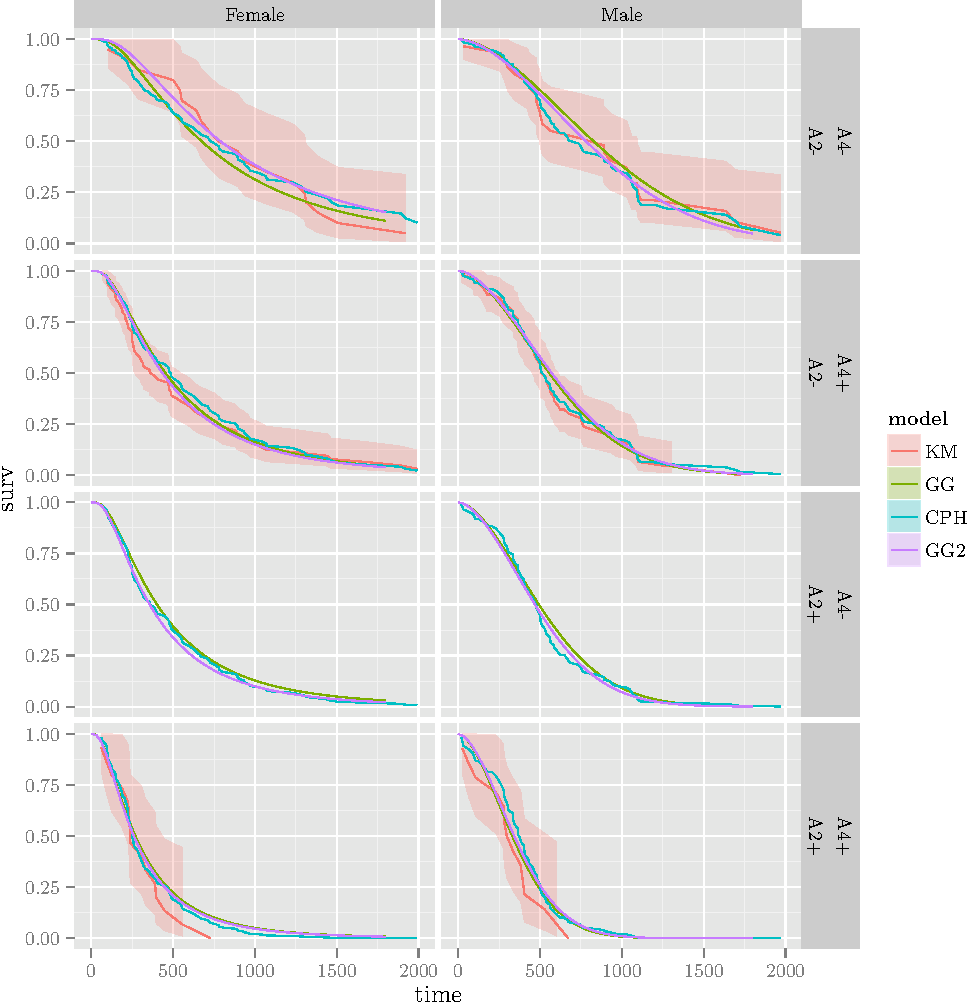
\includegraphics[width=\maxwidth]{figure/05-final-fit-assessment-3-2} 

}



\end{knitrout}

\begin{knitrout}
\definecolor{shadecolor}{rgb}{0.969, 0.969, 0.969}\color{fgcolor}\begin{kframe}
\begin{alltt}
\hlstd{temp.data}\hlopt{$}\hlstd{lower[temp.data}\hlopt{$}\hlstd{model} \hlopt{!=} \hlstr{"KM"}\hlstd{]} \hlkwb{=} \hlnum{NA}
\hlstd{temp.data}\hlopt{$}\hlstd{upper[temp.data}\hlopt{$}\hlstd{model} \hlopt{!=} \hlstr{"KM"}\hlstd{]} \hlkwb{=} \hlnum{NA}
\hlstd{temp.data} \hlkwb{=} \hlstd{temp.data[temp.data}\hlopt{$}\hlstd{model} \hlopt{!=} \hlstr{"GG2"}\hlstd{,]}
\hlstd{temp.data}\hlopt{$}\hlstd{model} \hlkwb{=} \hlkwd{c}\hlstd{(}\hlstr{"KM"} \hlstd{=} \hlstr{"Kaplan-Meier"}\hlstd{,} \hlstr{"GG"} \hlstd{=} \hlstr{"GG1"}\hlstd{,} \hlstr{"CPH"} \hlstd{=} \hlstr{"CP1"}\hlstd{)[temp.data}\hlopt{$}\hlstd{model]}
\hlkwd{ggplot}\hlstd{(temp.data,} \hlkwd{aes}\hlstd{(}\hlkwc{x} \hlstd{=} \hlkwd{log}\hlstd{(time),} \hlkwc{y} \hlstd{=} \hlkwd{log}\hlstd{(}\hlopt{-}\hlkwd{log}\hlstd{(surv)),} \hlkwc{ymin} \hlstd{=} \hlkwd{log}\hlstd{(}\hlopt{-}\hlkwd{log}\hlstd{(lower)),} \hlkwc{ymax} \hlstd{=} \hlkwd{log}\hlstd{(}\hlopt{-}\hlkwd{log}\hlstd{(upper)),} \hlkwc{colour} \hlstd{= model,} \hlkwc{fill} \hlstd{= model))} \hlopt{+}
        \hlkwd{geom_ribbon}\hlstd{(}\hlkwc{alpha} \hlstd{=} \hlnum{0.25}\hlstd{,} \hlkwc{colour} \hlstd{=} \hlnum{NA}\hlstd{)} \hlopt{+}
        \hlkwd{geom_line}\hlstd{()} \hlopt{+}
        \hlkwd{xlim}\hlstd{(}\hlnum{4}\hlstd{,} \hlnum{7}\hlstd{)} \hlopt{+} \hlkwd{ylim}\hlstd{(}\hlopt{-}\hlnum{4}\hlstd{,} \hlnum{2}\hlstd{)} \hlopt{+}
        \hlkwd{facet_grid}\hlstd{(A2} \hlopt{~} \hlstd{A4} \hlopt{~} \hlstd{Sex)}
\end{alltt}


{\ttfamily\noindent\color{warningcolor}{\#\# Warning: Removed 46 rows containing missing values (geom\_path).}}

{\ttfamily\noindent\color{warningcolor}{\#\# Warning: Removed 39 rows containing missing values (geom\_path).}}

{\ttfamily\noindent\color{warningcolor}{\#\# Warning: Removed 48 rows containing missing values (geom\_path).}}

{\ttfamily\noindent\color{warningcolor}{\#\# Warning: Removed 43 rows containing missing values (geom\_path).}}

{\ttfamily\noindent\color{warningcolor}{\#\# Warning: Removed 39 rows containing missing values (geom\_path).}}

{\ttfamily\noindent\color{warningcolor}{\#\# Warning: Removed 36 rows containing missing values (geom\_path).}}

{\ttfamily\noindent\color{warningcolor}{\#\# Warning: Removed 40 rows containing missing values (geom\_path).}}

{\ttfamily\noindent\color{warningcolor}{\#\# Warning: Removed 37 rows containing missing values (geom\_path).}}\end{kframe}

{\centering 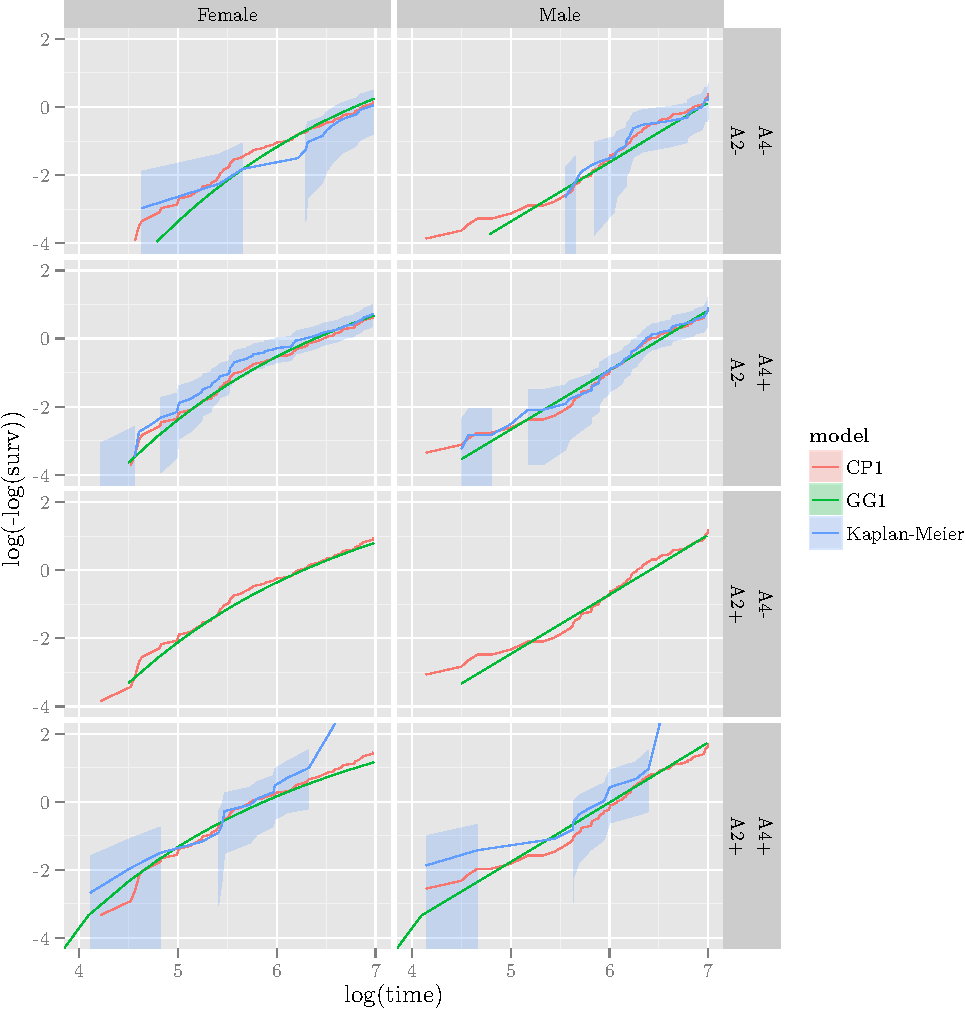
\includegraphics[width=\maxwidth]{figure/05-final-fit-assessment-4-1} 

}


\begin{kframe}\begin{alltt}
\hlkwd{ggplot}\hlstd{(temp.data,} \hlkwd{aes}\hlstd{(}\hlkwc{x} \hlstd{= time,} \hlkwc{y} \hlstd{= surv,} \hlkwc{ymin} \hlstd{= lower,} \hlkwc{ymax} \hlstd{= upper,} \hlkwc{colour} \hlstd{= model,} \hlkwc{fill} \hlstd{= model))} \hlopt{+}
        \hlkwd{geom_ribbon}\hlstd{(}\hlkwc{alpha} \hlstd{=} \hlnum{0.25}\hlstd{,} \hlkwc{colour} \hlstd{=} \hlnum{NA}\hlstd{)} \hlopt{+}
        \hlkwd{geom_line}\hlstd{()} \hlopt{+} \hlkwd{xlim}\hlstd{(}\hlnum{0}\hlstd{,} \hlnum{2000}\hlstd{)} \hlopt{+} \hlkwd{ylim}\hlstd{(}\hlnum{0}\hlstd{,} \hlnum{1}\hlstd{)} \hlopt{+}
        \hlkwd{facet_grid}\hlstd{(A2} \hlopt{~} \hlstd{A4} \hlopt{~} \hlstd{Sex)}
\end{alltt}


{\ttfamily\noindent\color{warningcolor}{\#\# Warning: Removed 3 rows containing missing values (geom\_path).}}

{\ttfamily\noindent\color{warningcolor}{\#\# Warning: Removed 3 rows containing missing values (geom\_path).}}

{\ttfamily\noindent\color{warningcolor}{\#\# Warning: Removed 2 rows containing missing values (geom\_path).}}

{\ttfamily\noindent\color{warningcolor}{\#\# Warning: Removed 2 rows containing missing values (geom\_path).}}\end{kframe}

{\centering 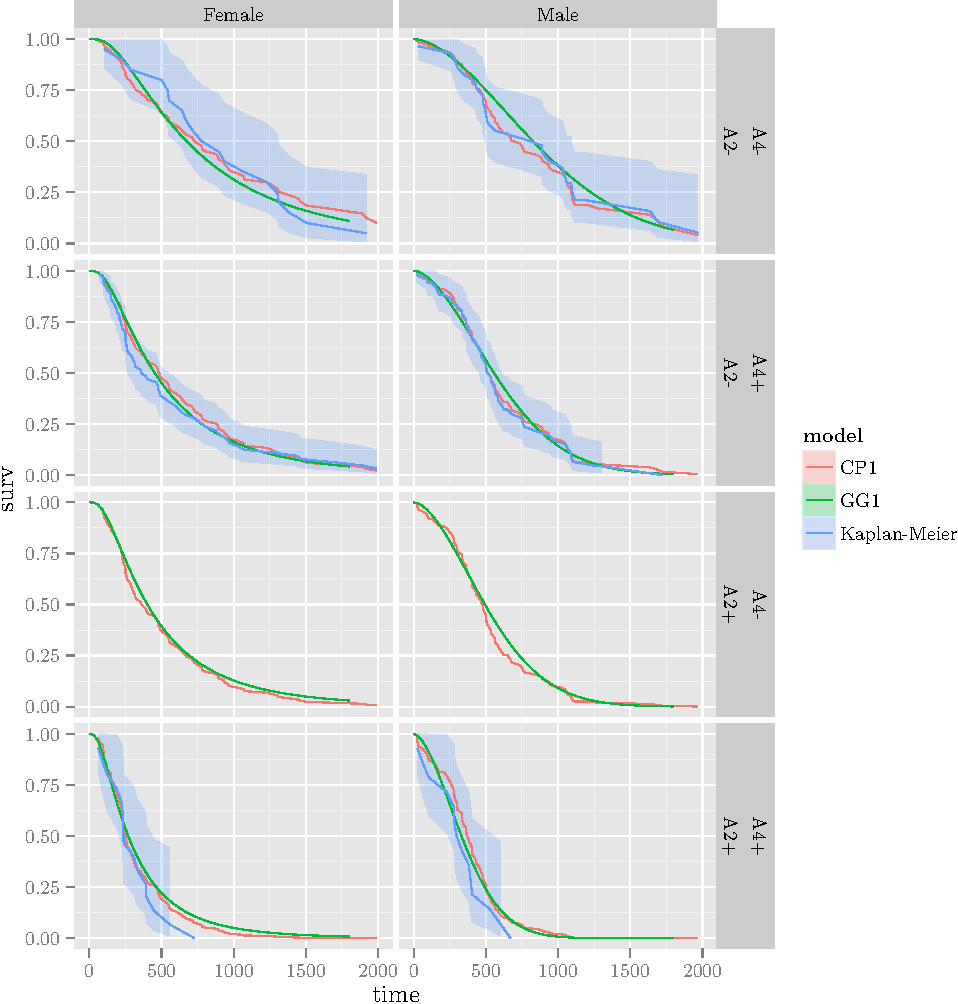
\includegraphics[width=\maxwidth]{figure/05-final-fit-assessment-4-2} 

}



\end{knitrout}


\section{Model selection}
It looks like that's as far as we can go with tweaking the fits.  Time to put the different models against each other on the holdout data, and choose a winner.

DIY IBS, wooo.
\begin{knitrout}
\definecolor{shadecolor}{rgb}{0.969, 0.969, 0.969}\color{fgcolor}\begin{kframe}
\begin{alltt}
\hlstd{calcIBS} \hlkwb{=} \hlkwa{function}\hlstd{(}\hlkwc{surv}\hlstd{,} \hlkwc{pred}\hlstd{,} \hlkwc{pred_times}\hlstd{,} \hlkwc{max_time}\hlstd{)}
\hlstd{\{}
        \hlkwd{stopifnot}\hlstd{(}\hlkwd{nrow}\hlstd{(surv)} \hlopt{==} \hlkwd{nrow}\hlstd{(pred)} \hlopt{&&} \hlkwd{length}\hlstd{(pred_times)} \hlopt{==} \hlkwd{ncol}\hlstd{(pred))}

        \hlstd{n} \hlkwb{=} \hlkwd{nrow}\hlstd{(surv)}
        \hlstd{marg_survfit} \hlkwb{=} \hlkwd{survfit}\hlstd{(surv} \hlopt{~} \hlnum{1}\hlstd{)}
        \hlstd{marg_censfit} \hlkwb{=} \hlkwd{survfit}\hlstd{(}\hlkwd{Surv}\hlstd{(surv[,}\hlnum{1}\hlstd{],} \hlopt{!}\hlstd{surv[,}\hlnum{2}\hlstd{])} \hlopt{~} \hlnum{1}\hlstd{)}
        \hlstd{marg_surv_func} \hlkwb{=} \hlkwd{approxfun}\hlstd{(marg_survfit}\hlopt{$}\hlstd{time, marg_survfit}\hlopt{$}\hlstd{surv,} \hlkwc{method} \hlstd{=} \hlstr{"constant"}\hlstd{,} \hlkwc{yleft} \hlstd{=} \hlnum{1}\hlstd{,} \hlkwc{yright} \hlstd{=} \hlnum{0}\hlstd{,} \hlkwc{rule} \hlstd{=} \hlnum{2}\hlopt{:}\hlnum{1}\hlstd{,} \hlkwc{f} \hlstd{=} \hlnum{0}\hlstd{)}
        \hlstd{marg_cens_func} \hlkwb{=} \hlkwd{approxfun}\hlstd{(marg_censfit}\hlopt{$}\hlstd{time, marg_censfit}\hlopt{$}\hlstd{surv,} \hlkwc{method} \hlstd{=} \hlstr{"constant"}\hlstd{,} \hlkwc{yleft} \hlstd{=} \hlnum{1}\hlstd{,} \hlkwc{yright} \hlstd{=} \hlnum{0}\hlstd{,} \hlkwc{rule} \hlstd{=} \hlnum{2}\hlopt{:}\hlnum{1}\hlstd{,} \hlkwc{f} \hlstd{=} \hlnum{0}\hlstd{)}

        \hlstd{pred_funcs} \hlkwb{=} \hlkwd{apply}\hlstd{(pred,} \hlnum{1}\hlstd{,} \hlkwa{function}\hlstd{(}\hlkwc{pat_preds}\hlstd{)} \hlkwd{approxfun}\hlstd{(pred_times, pat_preds,} \hlkwc{yleft} \hlstd{=} \hlnum{1}\hlstd{,} \hlkwc{yright} \hlstd{=} \hlkwd{min}\hlstd{(pat_preds),} \hlkwc{rule} \hlstd{=} \hlnum{2}\hlstd{))}

        \hlstd{indiv_patient_bsc} \hlkwb{=} \hlkwa{function}\hlstd{(}\hlkwc{pat_i}\hlstd{,} \hlkwc{tstars}\hlstd{)}
        \hlstd{\{}
                \hlstd{observed_time} \hlkwb{=} \hlstd{surv[pat_i,} \hlnum{1}\hlstd{]}
                \hlstd{observed_event} \hlkwb{=} \hlstd{surv[pat_i,} \hlnum{2}\hlstd{]}
                \hlstd{pred_func} \hlkwb{=} \hlstd{pred_funcs[[pat_i]]}
                \hlstd{category} \hlkwb{=} \hlnum{1}\hlopt{*}\hlstd{(observed_time} \hlopt{<=} \hlstd{tstars} \hlopt{&} \hlstd{observed_event)} \hlopt{+} \hlnum{2}\hlopt{*}\hlstd{(observed_time} \hlopt{>} \hlstd{tstars)} \hlopt{+} \hlnum{3}\hlopt{*}\hlstd{(observed_time} \hlopt{<=} \hlstd{tstars} \hlopt{& !}\hlstd{observed_event)}
                \hlstd{bsc} \hlkwb{=} \hlkwd{rep}\hlstd{(}\hlnum{NA}\hlstd{,} \hlkwd{length}\hlstd{(tstars))}
                \hlstd{bsc[category} \hlopt{==} \hlnum{1}\hlstd{]} \hlkwb{=} \hlkwd{pred_func}\hlstd{(tstars[category} \hlopt{==} \hlnum{1}\hlstd{])}\hlopt{^}\hlnum{2} \hlopt{/} \hlkwd{marg_cens_func}\hlstd{(observed_time)}
                \hlstd{bsc[category} \hlopt{==} \hlnum{2}\hlstd{]} \hlkwb{=} \hlstd{(}\hlnum{1} \hlopt{-} \hlkwd{pred_func}\hlstd{(tstars[category} \hlopt{==} \hlnum{2}\hlstd{]))}\hlopt{^}\hlnum{2} \hlopt{/} \hlkwd{marg_cens_func}\hlstd{(tstars[category} \hlopt{==} \hlnum{2}\hlstd{])}
                \hlstd{bsc[category} \hlopt{==} \hlnum{3}\hlstd{]} \hlkwb{=} \hlnum{0}
                \hlstd{bsc}
        \hlstd{\}}

        \hlstd{bsc_func} \hlkwb{=} \hlkwa{function}\hlstd{(}\hlkwc{tstars}\hlstd{) \{} \hlkwd{rowMeans}\hlstd{(}\hlkwd{sapply}\hlstd{(}\hlnum{1}\hlopt{:}\hlstd{n,} \hlkwa{function}\hlstd{(}\hlkwc{pat_i}\hlstd{)} \hlkwd{indiv_patient_bsc}\hlstd{(pat_i, tstars))) \}}

        \hlstd{weight_func} \hlkwb{=} \hlkwa{function}\hlstd{(}\hlkwc{tstars}\hlstd{) \{ (}\hlnum{1} \hlopt{-} \hlkwd{marg_surv_func}\hlstd{(tstars))} \hlopt{/} \hlstd{(}\hlnum{1} \hlopt{-} \hlkwd{marg_surv_func}\hlstd{(max_time)) \}}

        \hlcom{# Be slack and do trapezoidal int. with a fine grid.  It should be possible }
        \hlcom{# to calulate the int. exactly but I cbfed.}
        \hlstd{int_grid} \hlkwb{=} \hlkwd{seq}\hlstd{(}\hlnum{0}\hlstd{, max_time,} \hlkwc{length.out} \hlstd{=} \hlnum{1e3}\hlstd{)}
        \hlstd{bsc_vals} \hlkwb{=} \hlkwd{bsc_func}\hlstd{(int_grid)}
        \hlstd{weight_vals} \hlkwb{=} \hlkwd{weight_func}\hlstd{(int_grid)}
        \hlstd{int_vals} \hlkwb{=} \hlstd{bsc_vals} \hlopt{*} \hlstd{weight_vals}
        \hlstd{ibsc} \hlkwb{=} \hlstd{(}\hlnum{2}\hlopt{*}\hlkwd{sum}\hlstd{(int_vals)} \hlopt{-} \hlstd{int_vals[}\hlnum{1}\hlstd{]} \hlopt{-} \hlstd{int_vals[}\hlkwd{length}\hlstd{(int_vals)])} \hlopt{*} \hlstd{(}\hlkwd{diff}\hlstd{(}\hlkwd{range}\hlstd{(int_grid)))} \hlopt{/} \hlstd{(}\hlnum{2}\hlopt{*}\hlkwd{length}\hlstd{(int_vals))}

        \hlkwd{return}\hlstd{(}\hlkwd{list}\hlstd{(}\hlkwc{bsc} \hlstd{= bsc_vals,} \hlkwc{weights} \hlstd{= weight_vals,} \hlkwc{eval_times} \hlstd{= int_grid,} \hlkwc{ibsc} \hlstd{= ibsc))}
\hlstd{\}}
\end{alltt}
\end{kframe}
\end{knitrout}

Calculate survival probability predictions for each of the models, on the validation data.
\begin{knitrout}
\definecolor{shadecolor}{rgb}{0.969, 0.969, 0.969}\color{fgcolor}\begin{kframe}
\begin{alltt}
\hlstd{ibs_times} \hlkwb{=} \hlkwd{sort}\hlstd{(}\hlkwd{unique}\hlstd{(data.val}\hlopt{$}\hlstd{Time))}
\hlstd{ibs_preds_gg} \hlkwb{=} \hlkwd{as.matrix}\hlstd{(}\hlkwd{t}\hlstd{(}\hlkwd{sapply}\hlstd{(}\hlkwd{summary}\hlstd{(fit.gg,} \hlkwc{newdata} \hlstd{= data.val,} \hlkwc{type} \hlstd{=} \hlstr{"survival"}\hlstd{,} \hlkwc{t} \hlstd{= ibs_times),} \hlkwa{function}\hlstd{(}\hlkwc{x}\hlstd{) x}\hlopt{$}\hlstd{est)))}
\hlstd{ibs_preds_gg2} \hlkwb{=} \hlkwd{as.matrix}\hlstd{(}\hlkwd{t}\hlstd{(}\hlkwd{sapply}\hlstd{(}\hlkwd{summary}\hlstd{(fit.gg2,} \hlkwc{newdata} \hlstd{= data.val,} \hlkwc{type} \hlstd{=} \hlstr{"survival"}\hlstd{,} \hlkwc{t} \hlstd{= ibs_times),} \hlkwa{function}\hlstd{(}\hlkwc{x}\hlstd{) x}\hlopt{$}\hlstd{est)))}
\hlstd{temp_cox_preds} \hlkwb{=} \hlkwd{survfit}\hlstd{(fit.cph,} \hlkwc{newdata} \hlstd{= data.val)}
\hlstd{ibs_preds_cph} \hlkwb{=} \hlkwd{simplify2array}\hlstd{(}\hlkwd{tapply}\hlstd{(}\hlnum{1}\hlopt{:}\hlkwd{length}\hlstd{(temp_cox_preds}\hlopt{$}\hlstd{time),} \hlkwd{rep}\hlstd{(}\hlkwd{names}\hlstd{(temp_cox_preds}\hlopt{$}\hlstd{strata), temp_cox_preds}\hlopt{$}\hlstd{strata),} \hlkwa{function}\hlstd{(}\hlkwc{strat_i}\hlstd{) \{}
        \hlkwd{approx}\hlstd{(}\hlkwc{x} \hlstd{= temp_cox_preds}\hlopt{$}\hlstd{time[strat_i],} \hlkwc{y} \hlstd{= temp_cox_preds}\hlopt{$}\hlstd{surv[strat_i],} \hlkwc{xout} \hlstd{= ibs_times,} \hlkwc{method} \hlstd{=} \hlstr{"constant"}\hlstd{,} \hlkwc{yleft} \hlstd{=} \hlnum{1}\hlstd{,} \hlkwc{rule} \hlstd{=} \hlnum{2}\hlstd{,} \hlkwc{f} \hlstd{=} \hlnum{0}\hlstd{)}\hlopt{$}\hlstd{y \} ))}
\hlstd{ibs_preds_cph} \hlkwb{=} \hlkwd{t}\hlstd{(ibs_preds_cph[,}\hlkwd{rownames}\hlstd{(data.val)])}
\hlstd{temp_rsf_preds} \hlkwb{=} \hlkwd{predict}\hlstd{(fit.rsf,} \hlkwc{newdata} \hlstd{= data.val)}
\hlstd{ibs_preds_rsf} \hlkwb{=} \hlkwd{t}\hlstd{(}\hlkwd{apply}\hlstd{(temp_rsf_preds}\hlopt{$}\hlstd{survival,} \hlnum{1}\hlstd{,} \hlkwa{function}\hlstd{(}\hlkwc{survs}\hlstd{)} \hlkwd{approx}\hlstd{(temp_rsf_preds}\hlopt{$}\hlstd{time.interest, survs,} \hlkwc{xout} \hlstd{= ibs_times,} \hlkwc{method} \hlstd{=} \hlstr{"constant"}\hlstd{,} \hlkwc{yleft} \hlstd{=} \hlnum{1}\hlstd{,} \hlkwc{rule} \hlstd{=} \hlnum{2}\hlstd{,} \hlkwc{f} \hlstd{=} \hlnum{0}\hlstd{)}\hlopt{$}\hlstd{y))}
\hlcom{# Patients (from data.val) are in rows, times (from ibs_times) in columns.}

\hlcom{# Add a no-information KM predictor}
\hlstd{temp_km0} \hlkwb{=} \hlkwd{survfit}\hlstd{(}\hlkwd{Surv}\hlstd{(Time, DSD)} \hlopt{~} \hlnum{1}\hlstd{, data)}
\hlstd{ibs_preds_km0} \hlkwb{=} \hlkwd{t}\hlstd{(}\hlkwd{matrix}\hlstd{(}\hlkwd{rep}\hlstd{(}\hlkwd{approx}\hlstd{(temp_km0}\hlopt{$}\hlstd{time, temp_km0}\hlopt{$}\hlstd{surv,} \hlkwc{xout} \hlstd{= ibs_times,} \hlkwc{method} \hlstd{=} \hlstr{"constant"}\hlstd{,} \hlkwc{yleft} \hlstd{=} \hlnum{1}\hlstd{,} \hlkwc{rule} \hlstd{=} \hlnum{2}\hlstd{,} \hlkwc{f} \hlstd{=} \hlnum{0}\hlstd{)}\hlopt{$}\hlstd{y,} \hlkwc{times} \hlstd{=} \hlkwd{nrow}\hlstd{(data.val)),} \hlkwc{ncol} \hlstd{=} \hlkwd{nrow}\hlstd{(data.val)))}
\hlstd{ibs_preds_all} \hlkwb{=} \hlkwd{list}\hlstd{(}\hlkwc{gg} \hlstd{= ibs_preds_gg,} \hlkwc{gg2} \hlstd{= ibs_preds_gg2,} \hlkwc{cph} \hlstd{= ibs_preds_cph,} \hlkwc{rsf} \hlstd{= ibs_preds_rsf,} \hlkwc{km0} \hlstd{= ibs_preds_km0)}
\end{alltt}
\end{kframe}
\end{knitrout}


\begin{knitrout}
\definecolor{shadecolor}{rgb}{0.969, 0.969, 0.969}\color{fgcolor}\begin{kframe}
\begin{alltt}
\hlstd{val.prob.times} \hlkwb{=} \hlkwd{seq}\hlstd{(}\hlnum{0}\hlstd{,} \hlkwd{max}\hlstd{(data.val}\hlopt{$}\hlstd{Time),} \hlnum{1}\hlstd{)}

\hlstd{temp.coefs} \hlkwb{=} \hlkwd{coef}\hlstd{(fit.gg)}
\hlstd{val.linpred.gg} \hlkwb{=} \hlkwd{sapply}\hlstd{(}\hlnum{1}\hlopt{:}\hlkwd{length}\hlstd{(temp.coefs),} \hlkwa{function}\hlstd{(}\hlkwc{coef_i}\hlstd{) \{}
    \hlkwa{if} \hlstd{(}\hlkwd{names}\hlstd{(temp.coefs)[coef_i]} \hlopt \hlkwd{colnames}\hlstd{(data.val)) \{}
        \hlstd{temp.coefs[coef_i]} \hlopt{*} \hlstd{data.val[,}\hlkwd{names}\hlstd{(temp.coefs)[coef_i]]}
    \hlstd{\}} \hlkwa{else if} \hlstd{(}\hlkwd{gsub}\hlstd{(}\hlstr{"TRUE$"}\hlstd{,} \hlstr{""}\hlstd{,} \hlkwd{names}\hlstd{(temp.coefs)[coef_i])} \hlopt \hlkwd{colnames}\hlstd{(data.val)) \{}
        \hlstd{temp.coefs[coef_i]} \hlopt{*} \hlstd{data.val[,}\hlkwd{gsub}\hlstd{(}\hlstr{"TRUE$"}\hlstd{,} \hlstr{""}\hlstd{,} \hlkwd{names}\hlstd{(temp.coefs)[coef_i])]}
    \hlstd{\}} \hlkwa{else} \hlstd{\{}
        \hlkwd{rep}\hlstd{(}\hlnum{0}\hlstd{,} \hlkwd{nrow}\hlstd{(data.val))}
    \hlstd{\} \})}
\hlstd{val.linpred.gg} \hlkwb{=} \hlopt{-}\hlkwd{rowSums}\hlstd{(val.linpred.gg)}   \hlcom{# Negate to bring into concordance with the direction of Cox coefficients (ie higher is now worse)}
\hlstd{temp} \hlkwb{=} \hlkwd{summary}\hlstd{(fit.gg,} \hlkwc{newdata} \hlstd{= data.val,} \hlkwc{ci} \hlstd{=} \hlnum{FALSE}\hlstd{)}
\hlstd{val.prob.gg} \hlkwb{=} \hlkwd{sapply}\hlstd{(temp,} \hlkwa{function}\hlstd{(}\hlkwc{x}\hlstd{)} \hlkwd{approx}\hlstd{(x[,}\hlnum{1}\hlstd{], x[,}\hlnum{2}\hlstd{],} \hlkwc{xout} \hlstd{= val.prob.times,} \hlkwc{yleft} \hlstd{=} \hlnum{1}\hlstd{,} \hlkwc{yright} \hlstd{=} \hlnum{0}\hlstd{,} \hlkwc{rule} \hlstd{=} \hlnum{2}\hlstd{)}\hlopt{$}\hlstd{y)}
\hlkwd{colnames}\hlstd{(val.prob.gg)} \hlkwb{=} \hlkwd{rownames}\hlstd{(data.val)}

\hlstd{temp.coefs} \hlkwb{=} \hlkwd{coef}\hlstd{(fit.gg2)}
\hlstd{val.linpred.gg2} \hlkwb{=} \hlkwd{sapply}\hlstd{(}\hlnum{1}\hlopt{:}\hlkwd{length}\hlstd{(temp.coefs),} \hlkwa{function}\hlstd{(}\hlkwc{coef_i}\hlstd{) \{}
    \hlkwa{if} \hlstd{(}\hlkwd{names}\hlstd{(temp.coefs)[coef_i]} \hlopt \hlkwd{colnames}\hlstd{(data.val)) \{}
        \hlstd{temp.coefs[coef_i]} \hlopt{*} \hlstd{data.val[,}\hlkwd{names}\hlstd{(temp.coefs)[coef_i]]}
    \hlstd{\}} \hlkwa{else if} \hlstd{(}\hlkwd{gsub}\hlstd{(}\hlstr{"TRUE$"}\hlstd{,} \hlstr{""}\hlstd{,} \hlkwd{names}\hlstd{(temp.coefs)[coef_i])} \hlopt \hlkwd{colnames}\hlstd{(data.val)) \{}
        \hlstd{temp.coefs[coef_i]} \hlopt{*} \hlstd{data.val[,}\hlkwd{gsub}\hlstd{(}\hlstr{"TRUE$"}\hlstd{,} \hlstr{""}\hlstd{,} \hlkwd{names}\hlstd{(temp.coefs)[coef_i])]}
    \hlstd{\}} \hlkwa{else} \hlstd{\{}
        \hlkwd{rep}\hlstd{(}\hlnum{0}\hlstd{,} \hlkwd{nrow}\hlstd{(data.val))}
    \hlstd{\} \})}
\hlstd{val.linpred.gg2} \hlkwb{=} \hlopt{-}\hlkwd{rowSums}\hlstd{(val.linpred.gg2)}   \hlcom{# Negate to bring into concordance with the direction of Cox coefficients (ie higher is now worse)}
\hlstd{temp} \hlkwb{=} \hlkwd{summary}\hlstd{(fit.gg2,} \hlkwc{newdata} \hlstd{= data.val,} \hlkwc{ci} \hlstd{=} \hlnum{FALSE}\hlstd{)}
\hlstd{val.prob.gg2} \hlkwb{=} \hlkwd{sapply}\hlstd{(temp,} \hlkwa{function}\hlstd{(}\hlkwc{x}\hlstd{)} \hlkwd{approx}\hlstd{(x[,}\hlnum{1}\hlstd{], x[,}\hlnum{2}\hlstd{],} \hlkwc{xout} \hlstd{= val.prob.times,} \hlkwc{yleft} \hlstd{=} \hlnum{1}\hlstd{,} \hlkwc{yright} \hlstd{=} \hlnum{0}\hlstd{,} \hlkwc{rule} \hlstd{=} \hlnum{2}\hlstd{)}\hlopt{$}\hlstd{y)}
\hlkwd{colnames}\hlstd{(val.prob.gg2)} \hlkwb{=} \hlkwd{rownames}\hlstd{(data.val)}

\hlstd{val.linpred.cph} \hlkwb{=} \hlkwd{predict}\hlstd{(fit.cph,} \hlkwc{newdata} \hlstd{= data.val)}
\hlstd{temp} \hlkwb{=} \hlkwd{survfit}\hlstd{(fit.cph,} \hlkwc{newdata} \hlstd{= data.val)}
\hlstd{val.prob.cph} \hlkwb{=} \hlkwd{simplify2array}\hlstd{(}\hlkwd{tapply}\hlstd{(}\hlnum{1}\hlopt{:}\hlkwd{length}\hlstd{(temp}\hlopt{$}\hlstd{surv),} \hlkwd{rep}\hlstd{(}\hlkwd{names}\hlstd{(temp}\hlopt{$}\hlstd{strata), temp}\hlopt{$}\hlstd{strata),} \hlkwa{function}\hlstd{(}\hlkwc{is}\hlstd{)} \hlkwd{approx}\hlstd{(temp}\hlopt{$}\hlstd{time[is], temp}\hlopt{$}\hlstd{surv[is], val.prob.times,} \hlkwc{yleft} \hlstd{=} \hlnum{1}\hlstd{,} \hlkwc{yright} \hlstd{=} \hlnum{0}\hlstd{,} \hlkwc{rule} \hlstd{=} \hlnum{2}\hlstd{)}\hlopt{$}\hlstd{y))[,}\hlkwd{rownames}\hlstd{(data.val)]}

\hlstd{temp} \hlkwb{=} \hlkwd{predict}\hlstd{(fit.rsf,} \hlkwc{newdata} \hlstd{= data.val)}
\hlcom{# val.linpred.rsf = temp$predicted}
\hlcom{# Median survival time:}
\hlstd{val.linpred.rsf} \hlkwb{=} \hlkwd{apply}\hlstd{(temp}\hlopt{$}\hlstd{survival,} \hlnum{1}\hlstd{,} \hlkwa{function}\hlstd{(}\hlkwc{s1}\hlstd{) \{}
    \hlstd{sfunc} \hlkwb{=} \hlkwd{approxfun}\hlstd{(temp}\hlopt{$}\hlstd{time.interest, s1,} \hlkwc{yleft} \hlstd{=} \hlnum{1}\hlstd{,} \hlkwc{yright} \hlstd{=} \hlnum{0}\hlstd{,} \hlkwc{rule} \hlstd{=} \hlnum{2}\hlstd{)}
    \hlstd{med} \hlkwb{=} \hlkwd{uniroot}\hlstd{(}\hlkwa{function}\hlstd{(}\hlkwc{x}\hlstd{)} \hlkwd{sfunc}\hlstd{(x)} \hlopt{-} \hlnum{0.5}\hlstd{,} \hlkwc{lower} \hlstd{=} \hlkwd{min}\hlstd{(temp}\hlopt{$}\hlstd{time.interest),} \hlkwc{upper} \hlstd{=} \hlkwd{max}\hlstd{(temp}\hlopt{$}\hlstd{time.interest))}\hlopt{$}\hlstd{root}
    \hlstd{med}
\hlstd{\})}
\hlstd{val.linpred.rsf} \hlkwb{=} \hlopt{-}\hlstd{val.linpred.rsf}
\hlstd{val.prob.rsf} \hlkwb{=} \hlkwd{apply}\hlstd{(temp}\hlopt{$}\hlstd{survival,} \hlnum{1}\hlstd{,} \hlkwa{function}\hlstd{(}\hlkwc{s1}\hlstd{)} \hlkwd{approx}\hlstd{(temp}\hlopt{$}\hlstd{time.interest, s1,} \hlkwc{xout} \hlstd{= val.prob.times,} \hlkwc{yleft} \hlstd{=} \hlnum{1}\hlstd{,} \hlkwc{yright} \hlstd{=} \hlnum{0}\hlstd{,} \hlkwc{rule} \hlstd{=} \hlnum{2}\hlstd{)}\hlopt{$}\hlstd{y)}
\hlkwd{colnames}\hlstd{(val.prob.rsf)} \hlkwb{=} \hlkwd{rownames}\hlstd{(data.val)}

\hlkwd{summary}\hlstd{(}\hlkwd{coxph}\hlstd{(}\hlkwd{Surv}\hlstd{(Time, DSD)} \hlopt{~} \hlstd{val.linpred.gg, data.val))}
\end{alltt}
\begin{verbatim}
## Call:
## coxph(formula = Surv(Time, DSD) ~ val.linpred.gg, data = data.val)
## 
##   n= 61, number of events= 60 
## 
##                 coef exp(coef) se(coef)    z Pr(>|z|)
## val.linpred.gg 1.320     3.744    0.431 3.06   0.0022
## 
##                exp(coef) exp(-coef) lower .95 upper .95
## val.linpred.gg      3.74      0.267      1.61      8.71
## 
## Concordance= 0.659  (se = 0.044 )
## Rsquare= 0.144   (max possible= 0.998 )
## Likelihood ratio test= 9.48  on 1 df,   p=0.00208
## Wald test            = 9.39  on 1 df,   p=0.00219
## Score (logrank) test = 9.54  on 1 df,   p=0.00201
\end{verbatim}
\begin{alltt}
\hlkwd{summary}\hlstd{(}\hlkwd{coxph}\hlstd{(}\hlkwd{Surv}\hlstd{(Time, DSD)} \hlopt{~} \hlstd{val.linpred.gg2, data.val))}
\end{alltt}
\begin{verbatim}
## Call:
## coxph(formula = Surv(Time, DSD) ~ val.linpred.gg2, data = data.val)
## 
##   n= 61, number of events= 60 
## 
##                 coef exp(coef) se(coef)    z Pr(>|z|)
## val.linpred.gg2 1.32      3.75     0.45 2.94   0.0033
## 
##                 exp(coef) exp(-coef) lower .95 upper .95
## val.linpred.gg2      3.75      0.267      1.55      9.04
## 
## Concordance= 0.642  (se = 0.044 )
## Rsquare= 0.133   (max possible= 0.998 )
## Likelihood ratio test= 8.7  on 1 df,   p=0.00319
## Wald test            = 8.63  on 1 df,   p=0.00331
## Score (logrank) test = 8.76  on 1 df,   p=0.00307
\end{verbatim}
\begin{alltt}
\hlkwd{summary}\hlstd{(}\hlkwd{coxph}\hlstd{(}\hlkwd{Surv}\hlstd{(Time, DSD)} \hlopt{~} \hlstd{val.linpred.cph, data.val))}
\end{alltt}
\begin{verbatim}
## Call:
## coxph(formula = Surv(Time, DSD) ~ val.linpred.cph, data = data.val)
## 
##   n= 61, number of events= 60 
## 
##                  coef exp(coef) se(coef)    z Pr(>|z|)
## val.linpred.cph 1.192     3.295    0.338 3.53  0.00042
## 
##                 exp(coef) exp(-coef) lower .95 upper .95
## val.linpred.cph      3.29      0.304       1.7      6.39
## 
## Concordance= 0.649  (se = 0.044 )
## Rsquare= 0.177   (max possible= 0.998 )
## Likelihood ratio test= 11.8  on 1 df,   p=0.000578
## Wald test            = 12.4  on 1 df,   p=0.000421
## Score (logrank) test = 12.7  on 1 df,   p=0.000367
\end{verbatim}
\begin{alltt}
\hlkwd{summary}\hlstd{(}\hlkwd{coxph}\hlstd{(}\hlkwd{Surv}\hlstd{(Time, DSD)} \hlopt{~} \hlstd{val.linpred.rsf, data.val))}
\end{alltt}
\begin{verbatim}
## Call:
## coxph(formula = Surv(Time, DSD) ~ val.linpred.rsf, data = data.val)
## 
##   n= 61, number of events= 60 
## 
##                    coef exp(coef) se(coef)    z Pr(>|z|)
## val.linpred.rsf 0.00672   1.00675  0.00195 3.45  0.00055
## 
##                 exp(coef) exp(-coef) lower .95 upper .95
## val.linpred.rsf      1.01      0.993         1      1.01
## 
## Concordance= 0.679  (se = 0.044 )
## Rsquare= 0.178   (max possible= 0.998 )
## Likelihood ratio test= 12  on 1 df,   p=0.000538
## Wald test            = 11.9  on 1 df,   p=0.000551
## Score (logrank) test = 12.1  on 1 df,   p=0.000494
\end{verbatim}
\begin{alltt}
\hlkwd{anova}\hlstd{(}\hlkwd{coxph}\hlstd{(}\hlkwd{Surv}\hlstd{(Time, DSD)} \hlopt{~} \hlkwd{offset}\hlstd{(val.linpred.gg)} \hlopt{+} \hlstd{val.linpred.gg, data.val))}
\end{alltt}
\begin{verbatim}
## Analysis of Deviance Table
##  Cox model: response is Surv(Time, DSD)
## Terms added sequentially (first to last)
## 
##                loglik Chisq Df Pr(>|Chi|)
## NULL             -184                    
## val.linpred.gg   -184  0.55  1       0.46
\end{verbatim}
\begin{alltt}
\hlkwd{anova}\hlstd{(}\hlkwd{coxph}\hlstd{(}\hlkwd{Surv}\hlstd{(Time, DSD)} \hlopt{~} \hlkwd{offset}\hlstd{(val.linpred.gg2)} \hlopt{+} \hlstd{val.linpred.gg2, data.val))}
\end{alltt}
\begin{verbatim}
## Analysis of Deviance Table
##  Cox model: response is Surv(Time, DSD)
## Terms added sequentially (first to last)
## 
##                 loglik Chisq Df Pr(>|Chi|)
## NULL              -185                    
## val.linpred.gg2   -184  0.51  1       0.48
\end{verbatim}
\begin{alltt}
\hlkwd{anova}\hlstd{(}\hlkwd{coxph}\hlstd{(}\hlkwd{Surv}\hlstd{(Time, DSD)} \hlopt{~} \hlkwd{offset}\hlstd{(val.linpred.cph)} \hlopt{+} \hlstd{val.linpred.cph, data.val))}
\end{alltt}
\begin{verbatim}
## Analysis of Deviance Table
##  Cox model: response is Surv(Time, DSD)
## Terms added sequentially (first to last)
## 
##                 loglik Chisq Df Pr(>|Chi|)
## NULL              -183                    
## val.linpred.cph   -183  0.32  1       0.57
\end{verbatim}
\begin{alltt}
\hlkwd{anova}\hlstd{(}\hlkwd{coxph}\hlstd{(}\hlkwd{Surv}\hlstd{(Time, DSD)} \hlopt{~} \hlkwd{offset}\hlstd{(val.linpred.rsf)} \hlopt{+} \hlstd{val.linpred.rsf, data.val))}
\end{alltt}


{\ttfamily\noindent\color{warningcolor}{\#\# Warning in fitter(X, Y, strats, offset, init, control, weights = weights, : Ran out of iterations and did not converge}}

{\ttfamily\noindent\bfseries\color{errorcolor}{\#\# Error in fitter(X, Y, strats, offset, init, control, weights = weights, : NA/NaN/Inf in foreign function call (arg 6)}}\begin{alltt}
\hlkwd{summary}\hlstd{(}\hlkwd{coxph}\hlstd{(}\hlkwd{Surv}\hlstd{(Time, DSD)} \hlopt{~} \hlkwd{offset}\hlstd{(val.linpred.gg)} \hlopt{+} \hlstd{SexM} \hlopt{+} \hlstd{AgeCent} \hlopt{+} \hlstd{LocBody} \hlopt{+} \hlstd{SizeCent} \hlopt{+} \hlstd{A2} \hlopt{+} \hlstd{A4, data.val))}
\end{alltt}
\begin{verbatim}
## Call:
## coxph(formula = Surv(Time, DSD) ~ offset(val.linpred.gg) + SexM + 
##     AgeCent + LocBody + SizeCent + A2 + A4, data = data.val)
## 
##   n= 61, number of events= 60 
## 
##                 coef exp(coef) se(coef)     z Pr(>|z|)
## SexMTRUE     0.40127   1.49372  0.27817  1.44    0.149
## AgeCent     -0.02260   0.97766  0.01371 -1.65    0.099
## LocBodyTRUE  0.81060   2.24925  0.40567  2.00    0.046
## SizeCent    -0.00261   0.99740  0.00895 -0.29    0.771
## A2TRUE       0.69591   2.00553  0.50613  1.37    0.169
## A4TRUE       0.26205   1.29960  0.29377  0.89    0.372
## 
##             exp(coef) exp(-coef) lower .95 upper .95
## SexMTRUE        1.494      0.669     0.866      2.58
## AgeCent         0.978      1.023     0.952      1.00
## LocBodyTRUE     2.249      0.445     1.016      4.98
## SizeCent        0.997      1.003     0.980      1.02
## A2TRUE          2.006      0.499     0.744      5.41
## A4TRUE          1.300      0.769     0.731      2.31
## 
## Concordance= 0.687  (se = 0.044 )
## Rsquare= 0.152   (max possible= 0.998 )
## Likelihood ratio test= 10.1  on 6 df,   p=0.122
## Wald test            = 10.7  on 6 df,   p=0.0972
## Score (logrank) test = 11.2  on 6 df,   p=0.0815
\end{verbatim}
\begin{alltt}
\hlkwd{summary}\hlstd{(}\hlkwd{coxph}\hlstd{(}\hlkwd{Surv}\hlstd{(Time, DSD)} \hlopt{~} \hlkwd{offset}\hlstd{(val.linpred.gg2)} \hlopt{+} \hlstd{SexM} \hlopt{+} \hlstd{AgeCent} \hlopt{+} \hlstd{LocBody} \hlopt{+} \hlstd{SizeCent} \hlopt{+} \hlstd{A2} \hlopt{+} \hlstd{A4, data.val))}
\end{alltt}
\begin{verbatim}
## Call:
## coxph(formula = Surv(Time, DSD) ~ offset(val.linpred.gg2) + SexM + 
##     AgeCent + LocBody + SizeCent + A2 + A4, data = data.val)
## 
##   n= 61, number of events= 60 
## 
##                 coef exp(coef) se(coef)     z Pr(>|z|)
## SexMTRUE     0.42688   1.53246  0.27817  1.53    0.125
## AgeCent     -0.02260   0.97766  0.01371 -1.65    0.099
## LocBodyTRUE  0.81060   2.24925  0.40567  2.00    0.046
## SizeCent    -0.00249   0.99751  0.00895 -0.28    0.781
## A2TRUE       0.70033   2.01442  0.50613  1.38    0.166
## A4TRUE       0.33020   1.39125  0.29377  1.12    0.261
## 
##             exp(coef) exp(-coef) lower .95 upper .95
## SexMTRUE        1.532      0.653     0.888      2.64
## AgeCent         0.978      1.023     0.952      1.00
## LocBodyTRUE     2.249      0.445     1.016      4.98
## SizeCent        0.998      1.002     0.980      1.02
## A2TRUE          2.014      0.496     0.747      5.43
## A4TRUE          1.391      0.719     0.782      2.47
## 
## Concordance= 0.687  (se = 0.044 )
## Rsquare= 0.162   (max possible= 0.998 )
## Likelihood ratio test= 10.8  on 6 df,   p=0.0943
## Wald test            = 11.4  on 6 df,   p=0.0767
## Score (logrank) test = 11.9  on 6 df,   p=0.0638
\end{verbatim}
\begin{alltt}
\hlkwd{summary}\hlstd{(}\hlkwd{coxph}\hlstd{(}\hlkwd{Surv}\hlstd{(Time, DSD)} \hlopt{~} \hlkwd{offset}\hlstd{(val.linpred.cph)} \hlopt{+} \hlstd{SexM} \hlopt{+} \hlstd{AgeCent} \hlopt{+} \hlstd{LocBody} \hlopt{+} \hlstd{SizeCent} \hlopt{+} \hlstd{A2} \hlopt{+} \hlstd{A4, data.val))}
\end{alltt}
\begin{verbatim}
## Call:
## coxph(formula = Surv(Time, DSD) ~ offset(val.linpred.cph) + SexM + 
##     AgeCent + LocBody + SizeCent + A2 + A4, data = data.val)
## 
##   n= 61, number of events= 60 
## 
##                 coef exp(coef) se(coef)     z Pr(>|z|)
## SexMTRUE    -0.03303   0.96751  0.27817 -0.12    0.905
## AgeCent     -0.02260   0.97766  0.01371 -1.65    0.099
## LocBodyTRUE  0.81060   2.24925  0.40567  2.00    0.046
## SizeCent    -0.00544   0.99457  0.00895 -0.61    0.543
## A2TRUE       0.51021   1.66563  0.50613  1.01    0.313
## A4TRUE       0.12325   1.13117  0.29377  0.42    0.675
## 
##             exp(coef) exp(-coef) lower .95 upper .95
## SexMTRUE        0.968      1.034     0.561      1.67
## AgeCent         0.978      1.023     0.952      1.00
## LocBodyTRUE     2.249      0.445     1.016      4.98
## SizeCent        0.995      1.005     0.977      1.01
## A2TRUE          1.666      0.600     0.618      4.49
## A4TRUE          1.131      0.884     0.636      2.01
## 
## Concordance= 0.687  (se = 0.044 )
## Rsquare= 0.115   (max possible= 0.998 )
## Likelihood ratio test= 7.48  on 6 df,   p=0.279
## Wald test            = 8.05  on 6 df,   p=0.234
## Score (logrank) test = 8.41  on 6 df,   p=0.209
\end{verbatim}
\begin{alltt}
\hlkwd{summary}\hlstd{(}\hlkwd{coxph}\hlstd{(}\hlkwd{Surv}\hlstd{(Time, DSD)} \hlopt{~} \hlkwd{offset}\hlstd{(val.linpred.rsf)} \hlopt{+} \hlstd{SexM} \hlopt{+} \hlstd{AgeCent} \hlopt{+} \hlstd{LocBody} \hlopt{+} \hlstd{SizeCent} \hlopt{+} \hlstd{A2} \hlopt{+} \hlstd{A4, data.val))}
\end{alltt}


{\ttfamily\noindent\color{warningcolor}{\#\# Warning in fitter(X, Y, strats, offset, init, control, weights = weights, : Ran out of iterations and did not converge}}

{\ttfamily\noindent\bfseries\color{errorcolor}{\#\# Error in fitter(X, Y, strats, offset, init, control, weights = weights, : NA/NaN/Inf in foreign function call (arg 6)}}\end{kframe}
\end{knitrout}


TD-ROC AUC
\begin{knitrout}
\definecolor{shadecolor}{rgb}{0.969, 0.969, 0.969}\color{fgcolor}\begin{kframe}
\begin{alltt}
\hlstd{temp.times} \hlkwb{=} \hlkwd{seq}\hlstd{(}\hlnum{0.1}\hlstd{,} \hlnum{48}\hlstd{,} \hlnum{0.1}\hlstd{)}
\hlstd{temp.gg} \hlkwb{=} \hlkwd{timeROC}\hlstd{(data.val}\hlopt{$}\hlstd{Time}\hlopt{/}\hlnum{365.25}\hlopt{*}\hlnum{12}\hlstd{, data.val}\hlopt{$}\hlstd{DSD, val.linpred.gg,} \hlkwc{cause} \hlstd{=} \hlnum{1}\hlstd{,} \hlkwc{times} \hlstd{= temp.times,} \hlkwc{iid} \hlstd{=} \hlnum{TRUE}\hlstd{)}
\hlstd{temp.gg2} \hlkwb{=} \hlkwd{timeROC}\hlstd{(data.val}\hlopt{$}\hlstd{Time}\hlopt{/}\hlnum{365.25}\hlopt{*}\hlnum{12}\hlstd{, data.val}\hlopt{$}\hlstd{DSD, val.linpred.gg2,} \hlkwc{cause} \hlstd{=} \hlnum{1}\hlstd{,} \hlkwc{times} \hlstd{= temp.times,} \hlkwc{iid} \hlstd{=} \hlnum{TRUE}\hlstd{)}
\hlstd{temp.cph} \hlkwb{=} \hlkwd{timeROC}\hlstd{(data.val}\hlopt{$}\hlstd{Time}\hlopt{/}\hlnum{365.25}\hlopt{*}\hlnum{12}\hlstd{, data.val}\hlopt{$}\hlstd{DSD, val.linpred.cph,} \hlkwc{cause} \hlstd{=} \hlnum{1}\hlstd{,} \hlkwc{times} \hlstd{= temp.times,} \hlkwc{iid} \hlstd{=} \hlnum{TRUE}\hlstd{)}
\hlkwd{plotAUCcurve}\hlstd{(temp.gg,} \hlkwc{conf.int} \hlstd{=} \hlnum{FALSE}\hlstd{,} \hlkwc{add} \hlstd{=} \hlnum{FALSE}\hlstd{,} \hlkwc{col} \hlstd{=} \hlstr{"blue"}\hlstd{)}
\hlkwd{plotAUCcurve}\hlstd{(temp.gg2,} \hlkwc{conf.int} \hlstd{=} \hlnum{FALSE}\hlstd{,} \hlkwc{add} \hlstd{=} \hlnum{TRUE}\hlstd{,} \hlkwc{col} \hlstd{=} \hlstr{"green"}\hlstd{)}
\hlkwd{plotAUCcurve}\hlstd{(temp.cph,} \hlkwc{conf.int} \hlstd{=} \hlnum{FALSE}\hlstd{,} \hlkwc{add} \hlstd{=} \hlnum{TRUE}\hlstd{,} \hlkwc{col} \hlstd{=} \hlstr{"red"}\hlstd{)}
\hlkwd{legend}\hlstd{(}\hlstr{"topright"}\hlstd{,} \hlkwc{legend} \hlstd{=} \hlkwd{c}\hlstd{(}\hlstr{"GG"}\hlstd{,} \hlstr{"GG2"}\hlstd{,} \hlstr{"CPH"}\hlstd{),} \hlkwc{col} \hlstd{=} \hlkwd{c}\hlstd{(}\hlstr{"blue"}\hlstd{,} \hlstr{"green"}\hlstd{,} \hlstr{"red"}\hlstd{),} \hlkwc{lty} \hlstd{=} \hlstr{"solid"}\hlstd{)}
\end{alltt}
\end{kframe}

{\centering 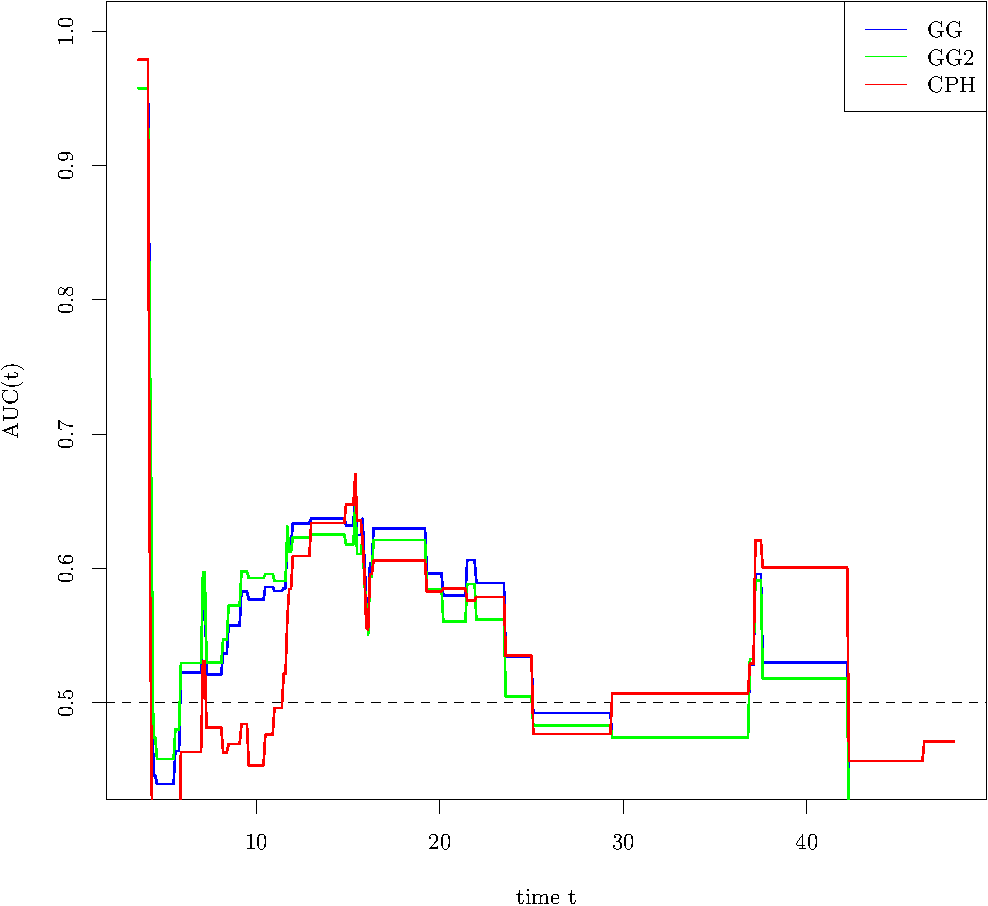
\includegraphics[width=\maxwidth]{figure/05-model-selection-auc-1} 

}



\end{knitrout}


Decision curve analysis.
\begin{knitrout}
\definecolor{shadecolor}{rgb}{0.969, 0.969, 0.969}\color{fgcolor}\begin{kframe}
\begin{alltt}
\hlstd{temp.data} \hlkwb{=} \hlkwd{data.frame}\hlstd{(}\hlkwc{Time} \hlstd{= data.val}\hlopt{$}\hlstd{Time,} \hlkwc{DSD} \hlstd{= data.val}\hlopt{$}\hlstd{DSD}\hlopt{*}\hlnum{1}\hlstd{,}
    \hlkwc{gg.1} \hlstd{=} \hlnum{1}\hlopt{-}\hlstd{val.prob.gg[val.prob.times} \hlopt{==} \hlnum{365}\hlstd{,],} \hlkwc{gg.2} \hlstd{=} \hlnum{1}\hlopt{-}\hlstd{val.prob.gg[val.prob.times} \hlopt{==} \hlnum{365}\hlopt{*}\hlnum{2}\hlstd{,],} \hlkwc{gg.3} \hlstd{=} \hlnum{1}\hlopt{-}\hlstd{val.prob.gg[val.prob.times} \hlopt{==} \hlnum{365}\hlopt{*}\hlnum{3}\hlstd{,],}
    \hlkwc{gg2.1} \hlstd{=} \hlnum{1}\hlopt{-}\hlstd{val.prob.gg2[val.prob.times} \hlopt{==} \hlnum{365}\hlstd{,],} \hlkwc{gg2.2} \hlstd{=} \hlnum{1}\hlopt{-}\hlstd{val.prob.gg2[val.prob.times} \hlopt{==} \hlnum{365}\hlopt{*}\hlnum{2}\hlstd{,],} \hlkwc{gg2.3} \hlstd{=} \hlnum{1}\hlopt{-}\hlstd{val.prob.gg2[val.prob.times} \hlopt{==} \hlnum{365}\hlopt{*}\hlnum{3}\hlstd{,],}
    \hlkwc{cph.1} \hlstd{=} \hlnum{1}\hlopt{-}\hlstd{val.prob.cph[val.prob.times} \hlopt{==} \hlnum{365}\hlstd{,],} \hlkwc{cph.2} \hlstd{=} \hlnum{1}\hlopt{-}\hlstd{val.prob.cph[val.prob.times} \hlopt{==} \hlnum{365}\hlopt{*}\hlnum{2}\hlstd{,],} \hlkwc{cph.3} \hlstd{=} \hlnum{1}\hlopt{-}\hlstd{val.prob.cph[val.prob.times} \hlopt{==} \hlnum{365}\hlopt{*}\hlnum{3}\hlstd{,],}
    \hlkwc{rsf.1} \hlstd{=} \hlnum{1}\hlopt{-}\hlstd{val.prob.rsf[val.prob.times} \hlopt{==} \hlnum{365}\hlstd{,],} \hlkwc{rsf.2} \hlstd{=} \hlnum{1}\hlopt{-}\hlstd{val.prob.rsf[val.prob.times} \hlopt{==} \hlnum{365}\hlopt{*}\hlnum{2}\hlstd{,],} \hlkwc{rsf.3} \hlstd{=} \hlnum{1}\hlopt{-}\hlstd{val.prob.rsf[val.prob.times} \hlopt{==} \hlnum{365}\hlopt{*}\hlnum{3}\hlstd{,])}
\hlkwd{stdca}\hlstd{(}\hlkwc{data} \hlstd{= temp.data,} \hlkwc{outcome} \hlstd{=} \hlstr{"DSD"}\hlstd{,} \hlkwc{ttoutcome} \hlstd{=} \hlstr{"Time"}\hlstd{,} \hlkwc{predictors} \hlstd{=} \hlkwd{c}\hlstd{(}\hlstr{"gg.1"}\hlstd{,} \hlstr{"cph.1"}\hlstd{,} \hlstr{"rsf.1"}\hlstd{),} \hlkwc{timepoint} \hlstd{=} \hlnum{365}\hlstd{,} \hlkwc{probability} \hlstd{=} \hlkwd{rep}\hlstd{(}\hlnum{TRUE}\hlstd{,} \hlnum{3}\hlstd{))}
\end{alltt}


{\ttfamily\noindent\bfseries\color{errorcolor}{\#\# Error in eval(expr, envir, enclos): could not find function "{}stdca"{}}}\begin{alltt}
\hlkwd{stdca}\hlstd{(}\hlkwc{data} \hlstd{= temp.data,} \hlkwc{outcome} \hlstd{=} \hlstr{"DSD"}\hlstd{,} \hlkwc{ttoutcome} \hlstd{=} \hlstr{"Time"}\hlstd{,} \hlkwc{predictors} \hlstd{=} \hlkwd{c}\hlstd{(}\hlstr{"gg.2"}\hlstd{,} \hlstr{"cph.2"}\hlstd{,} \hlstr{"rsf.2"}\hlstd{),} \hlkwc{timepoint} \hlstd{=} \hlnum{365}\hlopt{*}\hlnum{2}\hlstd{,} \hlkwc{probability} \hlstd{=} \hlkwd{rep}\hlstd{(}\hlnum{TRUE}\hlstd{,} \hlnum{3}\hlstd{))}
\end{alltt}


{\ttfamily\noindent\bfseries\color{errorcolor}{\#\# Error in eval(expr, envir, enclos): could not find function "{}stdca"{}}}\begin{alltt}
\hlkwd{stdca}\hlstd{(}\hlkwc{data} \hlstd{= temp.data,} \hlkwc{outcome} \hlstd{=} \hlstr{"DSD"}\hlstd{,} \hlkwc{ttoutcome} \hlstd{=} \hlstr{"Time"}\hlstd{,} \hlkwc{predictors} \hlstd{=} \hlkwd{c}\hlstd{(}\hlstr{"gg.3"}\hlstd{,} \hlstr{"cph.3"}\hlstd{,} \hlstr{"rsf.3"}\hlstd{),} \hlkwc{timepoint} \hlstd{=} \hlnum{365}\hlopt{*}\hlnum{3}\hlstd{,} \hlkwc{probability} \hlstd{=} \hlkwd{rep}\hlstd{(}\hlnum{TRUE}\hlstd{,} \hlnum{3}\hlstd{))}
\end{alltt}


{\ttfamily\noindent\bfseries\color{errorcolor}{\#\# Error in eval(expr, envir, enclos): could not find function "{}stdca"{}}}\end{kframe}
\end{knitrout}


Evaluate IBS point estimates.
BS paths over time on bootstrap samples of the holdout set.
\begin{knitrout}
\definecolor{shadecolor}{rgb}{0.969, 0.969, 0.969}\color{fgcolor}\begin{kframe}
\begin{alltt}
\hlkwd{set.seed}\hlstd{(}\hlnum{20150111}\hlstd{)}
\hlstd{ibs_eval_times} \hlkwb{=} \hlkwd{calcIBS}\hlstd{(}\hlkwd{Surv}\hlstd{(data.val}\hlopt{$}\hlstd{Time, data.val}\hlopt{$}\hlstd{DSD), ibs_preds_gg, ibs_times,} \hlkwd{max}\hlstd{(data.val}\hlopt{$}\hlstd{Time))}\hlopt{$}\hlstd{eval_times}
\hlcom{# bsc_boot2 = lapply(ibs_preds_all, function(preds) boot(data.val, statistic = function(d, i) calcIBS(Surv(d$Time, d$DSD)[i,], preds[i,], ibs_times, max(d$Time))$bsc, R = 500))}
\hlcom{# bsc_boot2ci = lapply(bsc_boot2, function(single_boot) t(sapply(1:length(ibs_eval_times), function(time_index) \{}
\hlcom{# 	temp = try(boot.ci(single_boot, index = time_index, type = "bca")$bca, silent = TRUE)}
\hlcom{# 	if (class(temp) == "try-error" || is.null(temp)) \{ temp = rep(NA, 5) \}}
\hlcom{# 	temp \})))}
\hlstd{bsc_boots} \hlkwb{=} \hlkwd{laply}\hlstd{(}\hlnum{1}\hlopt{:}\hlnum{500}\hlstd{,} \hlkwa{function}\hlstd{(}\hlkwc{i}\hlstd{) \{}
        \hlkwa{if} \hlstd{(i} \hlopt \hlnum{50} \hlopt{==} \hlnum{0}\hlstd{)       \{} \hlkwd{message}\hlstd{(i) \}}
        \hlstd{boot_samp} \hlkwb{=} \hlkwd{sample.int}\hlstd{(}\hlkwd{nrow}\hlstd{(data.val),} \hlkwc{replace} \hlstd{=} \hlnum{TRUE}\hlstd{)}
        \hlstd{gg} \hlkwb{=} \hlkwd{calcIBS}\hlstd{(}\hlkwd{Surv}\hlstd{(data.val}\hlopt{$}\hlstd{Time, data.val}\hlopt{$}\hlstd{DSD)[boot_samp,], ibs_preds_gg[boot_samp,], ibs_times,} \hlkwd{max}\hlstd{(data.val}\hlopt{$}\hlstd{Time))}\hlopt{$}\hlstd{bsc}
        \hlstd{gg2} \hlkwb{=} \hlkwd{calcIBS}\hlstd{(}\hlkwd{Surv}\hlstd{(data.val}\hlopt{$}\hlstd{Time, data.val}\hlopt{$}\hlstd{DSD)[boot_samp,], ibs_preds_gg2[boot_samp,], ibs_times,} \hlkwd{max}\hlstd{(data.val}\hlopt{$}\hlstd{Time))}\hlopt{$}\hlstd{bsc}
        \hlstd{cph} \hlkwb{=} \hlkwd{calcIBS}\hlstd{(}\hlkwd{Surv}\hlstd{(data.val}\hlopt{$}\hlstd{Time, data.val}\hlopt{$}\hlstd{DSD)[boot_samp,], ibs_preds_cph[boot_samp,], ibs_times,} \hlkwd{max}\hlstd{(data.val}\hlopt{$}\hlstd{Time))}\hlopt{$}\hlstd{bsc}
        \hlstd{rsf} \hlkwb{=} \hlkwd{calcIBS}\hlstd{(}\hlkwd{Surv}\hlstd{(data.val}\hlopt{$}\hlstd{Time, data.val}\hlopt{$}\hlstd{DSD)[boot_samp,], ibs_preds_rsf[boot_samp,], ibs_times,} \hlkwd{max}\hlstd{(data.val}\hlopt{$}\hlstd{Time))}\hlopt{$}\hlstd{bsc}
        \hlstd{km0} \hlkwb{=} \hlkwd{calcIBS}\hlstd{(}\hlkwd{Surv}\hlstd{(data.val}\hlopt{$}\hlstd{Time, data.val}\hlopt{$}\hlstd{DSD)[boot_samp,], ibs_preds_km0[boot_samp,], ibs_times,} \hlkwd{max}\hlstd{(data.val}\hlopt{$}\hlstd{Time))}\hlopt{$}\hlstd{bsc}
        \hlkwd{rbind}\hlstd{(gg, gg2, cph, rsf, km0)}
\hlstd{\})}
\end{alltt}


{\ttfamily\noindent\itshape\color{messagecolor}{\#\# 50\\\#\# 100\\\#\# 150\\\#\# 200\\\#\# 250\\\#\# 300\\\#\# 350\\\#\# 400\\\#\# 450\\\#\# 500}}\end{kframe}
\end{knitrout}

\begin{knitrout}
\definecolor{shadecolor}{rgb}{0.969, 0.969, 0.969}\color{fgcolor}\begin{kframe}
\begin{alltt}
\hlstd{temp} \hlkwb{=} \hlkwd{sapply}\hlstd{(}\hlkwd{list}\hlstd{(}\hlkwc{gg} \hlstd{= ibs_preds_gg,} \hlkwc{gg2} \hlstd{= ibs_preds_gg2,} \hlkwc{cph} \hlstd{= ibs_preds_cph,} \hlkwc{rsf} \hlstd{= ibs_preds_rsf,} \hlkwc{km0} \hlstd{= ibs_preds_km0),} \hlkwa{function}\hlstd{(}\hlkwc{preds}\hlstd{)} \hlkwd{calcIBS}\hlstd{(}\hlkwd{Surv}\hlstd{(data.val}\hlopt{$}\hlstd{Time, data.val}\hlopt{$}\hlstd{DSD), preds, ibs_times,} \hlkwd{max}\hlstd{(data.val}\hlopt{$}\hlstd{Time))}\hlopt{$}\hlstd{bsc)}
\hlstd{temp} \hlkwb{=} \hlkwd{melt}\hlstd{(temp)}
\hlkwd{colnames}\hlstd{(temp)} \hlkwb{=} \hlkwd{c}\hlstd{(}\hlstr{"Time"}\hlstd{,} \hlstr{"Model"}\hlstd{,} \hlstr{"BS"}\hlstd{)}
\hlkwd{ggplot}\hlstd{(temp,} \hlkwd{aes}\hlstd{(}\hlkwc{x} \hlstd{= Time,} \hlkwc{y} \hlstd{= BS,} \hlkwc{colour} \hlstd{= Model))} \hlopt{+} \hlkwd{geom_line}\hlstd{()} \hlopt{+} \hlkwd{ylab}\hlstd{(}\hlstr{"Brier Score"}\hlstd{)} \hlopt{+} \hlkwd{geom_hline}\hlstd{(}\hlkwc{yintercept} \hlstd{=} \hlnum{0.25}\hlstd{)}
\end{alltt}
\end{kframe}

{\centering 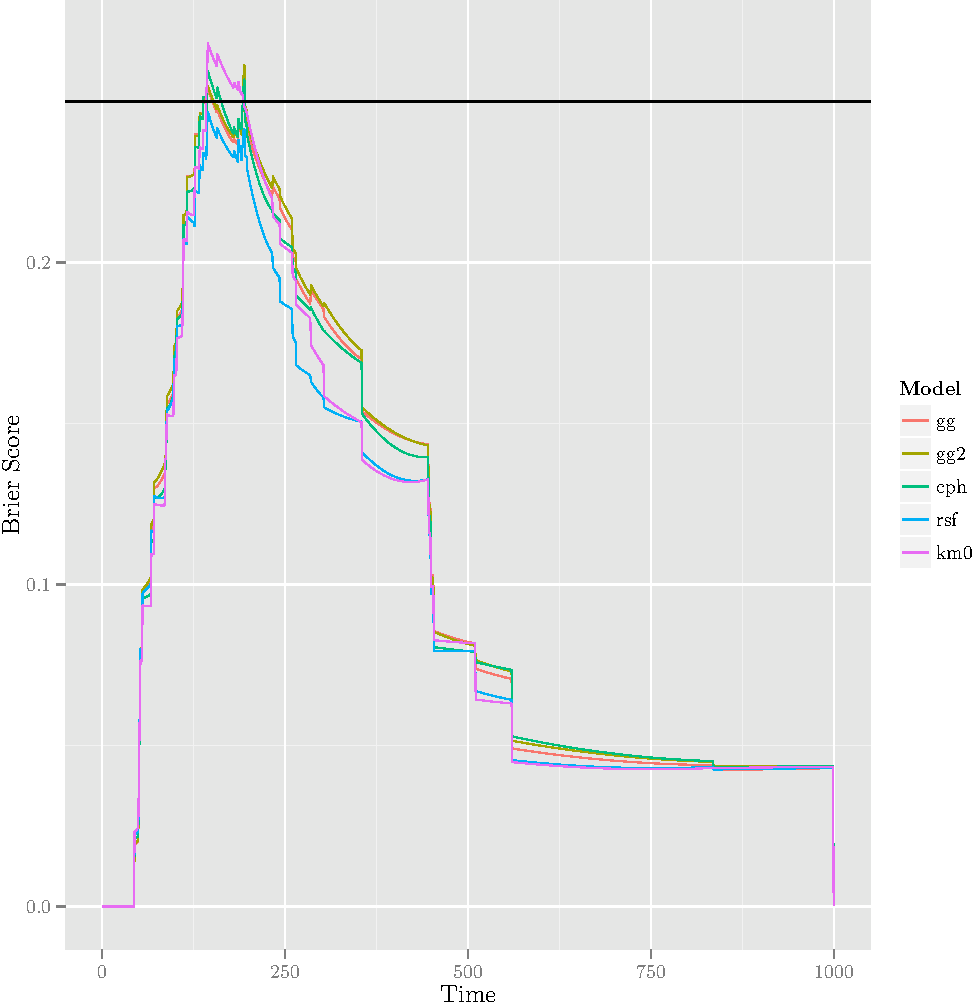
\includegraphics[width=\maxwidth]{figure/05-model-selection-bs-paths-1} 

}


\begin{kframe}\begin{alltt}
\hlstd{temp} \hlkwb{=} \hlkwd{melt}\hlstd{(}\hlkwd{aaply}\hlstd{(bsc_boots,} \hlnum{2}\hlopt{:}\hlnum{3}\hlstd{, quantile,} \hlkwc{probs} \hlstd{=} \hlkwd{c}\hlstd{(}\hlnum{0.05}\hlstd{,} \hlnum{0.5}\hlstd{,} \hlnum{0.95}\hlstd{)))}
\hlkwd{colnames}\hlstd{(temp)} \hlkwb{=} \hlkwd{c}\hlstd{(}\hlstr{"Model"}\hlstd{,} \hlstr{"Time"}\hlstd{,} \hlstr{"Quantile"}\hlstd{,} \hlstr{"Value"}\hlstd{)}
\hlstd{temp}\hlopt{$}\hlstd{Quantile} \hlkwb{=} \hlkwd{paste}\hlstd{(}\hlstr{"Q"}\hlstd{,} \hlkwd{gsub}\hlstd{(}\hlstr{"%"}\hlstd{,} \hlstr{""}\hlstd{, temp}\hlopt{$}\hlstd{Quantile),} \hlkwc{sep} \hlstd{=} \hlstr{""}\hlstd{)}
\hlstd{temp} \hlkwb{=} \hlkwd{dcast}\hlstd{(temp, Model} \hlopt{+} \hlstd{Time} \hlopt{~} \hlstd{Quantile,} \hlkwc{value.var} \hlstd{=} \hlstr{"Value"}\hlstd{)}
\hlkwd{ggplot}\hlstd{(temp,} \hlkwd{aes}\hlstd{(}\hlkwc{x} \hlstd{= Time,} \hlkwc{y} \hlstd{= Q50,} \hlkwc{ymin} \hlstd{= Q5,} \hlkwc{ymax} \hlstd{= Q95,} \hlkwc{colour} \hlstd{= Model,} \hlkwc{fill} \hlstd{= Model))} \hlopt{+} \hlkwd{geom_line}\hlstd{()} \hlopt{+} \hlkwd{geom_ribbon}\hlstd{(}\hlkwc{alpha} \hlstd{=} \hlnum{0.2}\hlstd{,} \hlkwc{colour} \hlstd{=} \hlnum{NA}\hlstd{)} \hlopt{+} \hlkwd{ylab}\hlstd{(}\hlstr{"Brier Score, 90\textbackslash{}\textbackslash{}% BI"}\hlstd{)} \hlopt{+} \hlkwd{geom_hline}\hlstd{(}\hlkwc{yintercept} \hlstd{=} \hlnum{0.25}\hlstd{)}
\end{alltt}
\end{kframe}

{\centering 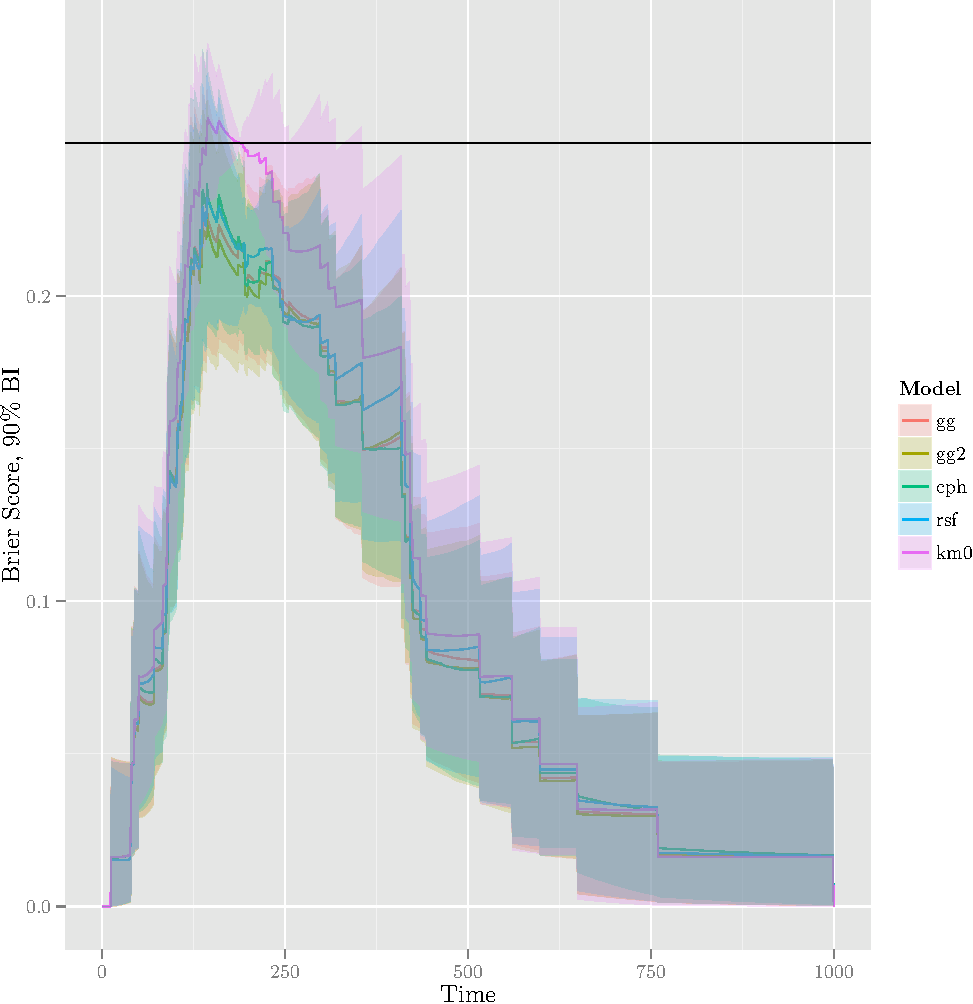
\includegraphics[width=\maxwidth]{figure/05-model-selection-bs-paths-2} 

}


\begin{kframe}\begin{alltt}
\hlstd{bsc_boots_diff} \hlkwb{=} \hlkwd{aaply}\hlstd{(bsc_boots,} \hlnum{2}\hlstd{,} \hlkwa{function}\hlstd{(}\hlkwc{x}\hlstd{) x} \hlopt{-} \hlstd{bsc_boots[,}\hlnum{5}\hlstd{,])[}\hlnum{1}\hlopt{:}\hlnum{4}\hlstd{,,]}
\hlstd{temp} \hlkwb{=} \hlkwd{melt}\hlstd{(}\hlkwd{aaply}\hlstd{(bsc_boots_diff,} \hlkwd{c}\hlstd{(}\hlnum{1}\hlstd{,}\hlnum{3}\hlstd{), quantile,} \hlkwc{probs} \hlstd{=} \hlkwd{c}\hlstd{(}\hlnum{0.05}\hlstd{,} \hlnum{0.5}\hlstd{,} \hlnum{0.95}\hlstd{)))}
\hlkwd{colnames}\hlstd{(temp)} \hlkwb{=} \hlkwd{c}\hlstd{(}\hlstr{"Model"}\hlstd{,} \hlstr{"Time"}\hlstd{,} \hlstr{"Quantile"}\hlstd{,} \hlstr{"Value"}\hlstd{)}
\hlstd{temp}\hlopt{$}\hlstd{Quantile} \hlkwb{=} \hlkwd{paste}\hlstd{(}\hlstr{"Q"}\hlstd{,} \hlkwd{gsub}\hlstd{(}\hlstr{"%"}\hlstd{,} \hlstr{""}\hlstd{, temp}\hlopt{$}\hlstd{Quantile),} \hlkwc{sep} \hlstd{=} \hlstr{""}\hlstd{)}
\hlstd{temp} \hlkwb{=} \hlkwd{dcast}\hlstd{(temp, Model} \hlopt{+} \hlstd{Time} \hlopt{~} \hlstd{Quantile,} \hlkwc{value.var} \hlstd{=} \hlstr{"Value"}\hlstd{)}
\hlkwd{ggplot}\hlstd{(temp,} \hlkwd{aes}\hlstd{(}\hlkwc{x} \hlstd{= Time,} \hlkwc{y} \hlstd{= Q50,} \hlkwc{ymin} \hlstd{= Q5,} \hlkwc{ymax} \hlstd{= Q95,} \hlkwc{colour} \hlstd{= Model,} \hlkwc{fill} \hlstd{= Model))} \hlopt{+} \hlkwd{geom_line}\hlstd{()} \hlopt{+} \hlkwd{geom_ribbon}\hlstd{(}\hlkwc{alpha} \hlstd{=} \hlnum{0.2}\hlstd{,} \hlkwc{colour} \hlstd{=} \hlnum{NA}\hlstd{)} \hlopt{+} \hlkwd{ylab}\hlstd{(}\hlstr{"Brier Score: Improvement over KM0. BS median, 90\textbackslash{}\textbackslash{}% BI"}\hlstd{)} \hlopt{+} \hlkwd{geom_hline}\hlstd{(}\hlkwc{yintercept} \hlstd{=} \hlnum{0}\hlstd{)}
\end{alltt}
\end{kframe}

{\centering 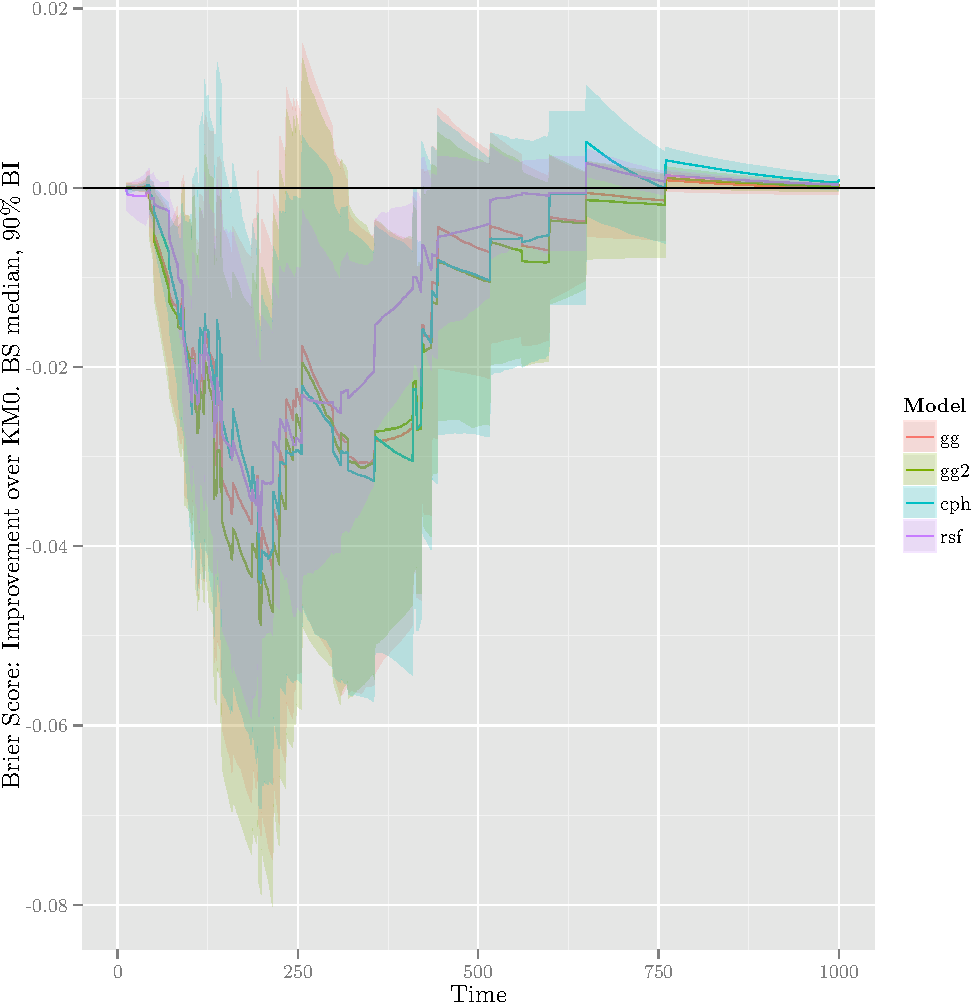
\includegraphics[width=\maxwidth]{figure/05-model-selection-bs-paths-3} 

}


\begin{kframe}\begin{alltt}
\hlkwd{ggplot}\hlstd{(temp,} \hlkwd{aes}\hlstd{(}\hlkwc{x} \hlstd{= Time,} \hlkwc{y} \hlstd{= Q50,} \hlkwc{ymin} \hlstd{= Q5,} \hlkwc{ymax} \hlstd{= Q95,} \hlkwc{colour} \hlstd{= Model,} \hlkwc{fill} \hlstd{= Model))} \hlopt{+} \hlkwd{geom_line}\hlstd{()} \hlopt{+} \hlkwd{geom_ribbon}\hlstd{(}\hlkwc{alpha} \hlstd{=} \hlnum{0.2}\hlstd{,} \hlkwc{colour} \hlstd{=} \hlnum{NA}\hlstd{)} \hlopt{+} \hlkwd{xlim}\hlstd{(}\hlnum{0}\hlstd{,} \hlnum{700}\hlstd{)} \hlopt{+} \hlkwd{ylab}\hlstd{(}\hlstr{"Brier Score: Improvement over KM0. BS median, 90\textbackslash{}\textbackslash{}% BI"}\hlstd{)} \hlopt{+} \hlkwd{geom_hline}\hlstd{(}\hlkwc{yintercept} \hlstd{=} \hlnum{0}\hlstd{)}
\end{alltt}


{\ttfamily\noindent\color{warningcolor}{\#\# Warning: Removed 1200 rows containing missing values (geom\_path).}}\end{kframe}

{\centering 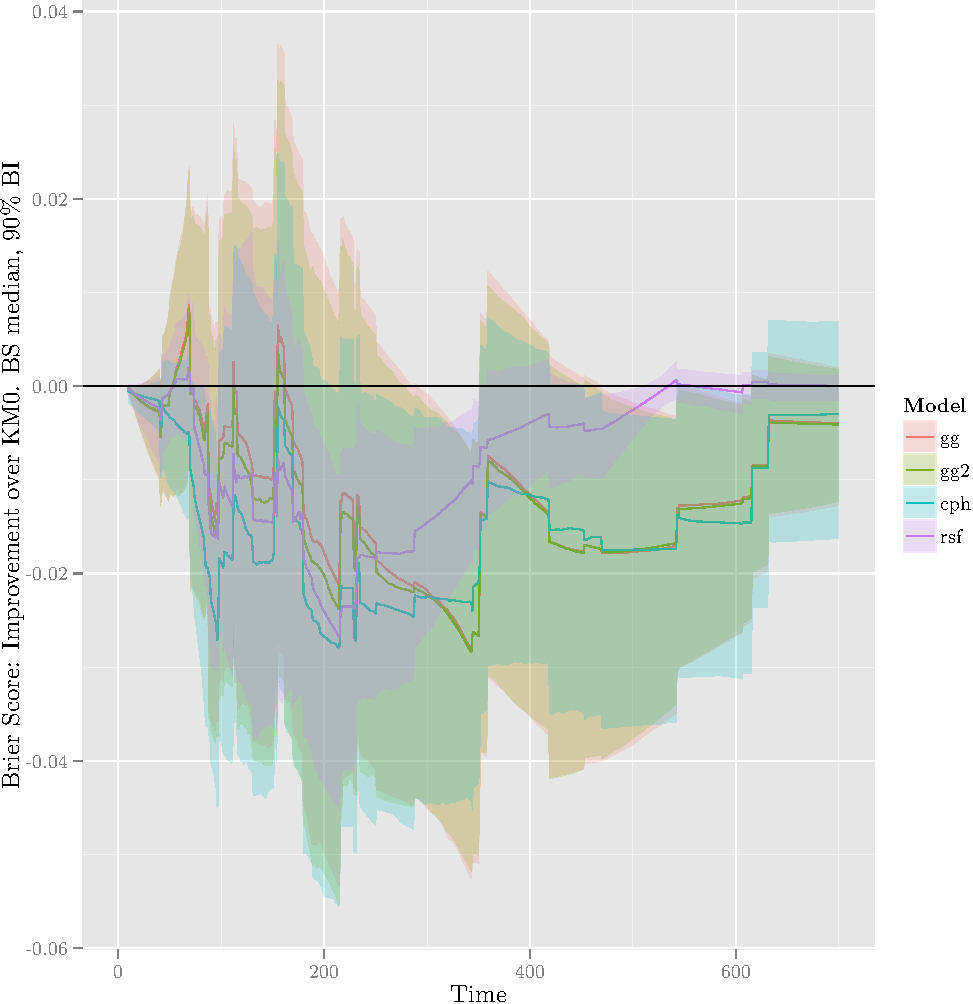
\includegraphics[width=\maxwidth]{figure/05-model-selection-bs-paths-4} 

}


\begin{kframe}\begin{alltt}
\hlkwd{ggplot}\hlstd{(temp,} \hlkwd{aes}\hlstd{(}\hlkwc{x} \hlstd{= Time,} \hlkwc{y} \hlstd{= Q50,} \hlkwc{colour} \hlstd{= Model))} \hlopt{+} \hlkwd{geom_line}\hlstd{()} \hlopt{+} \hlkwd{ylab}\hlstd{(}\hlstr{"Brier Score: Improvement over KM0, BS median"}\hlstd{)} \hlopt{+} \hlkwd{geom_hline}\hlstd{(}\hlkwc{yintercept} \hlstd{=} \hlnum{0}\hlstd{)}
\end{alltt}
\end{kframe}

{\centering 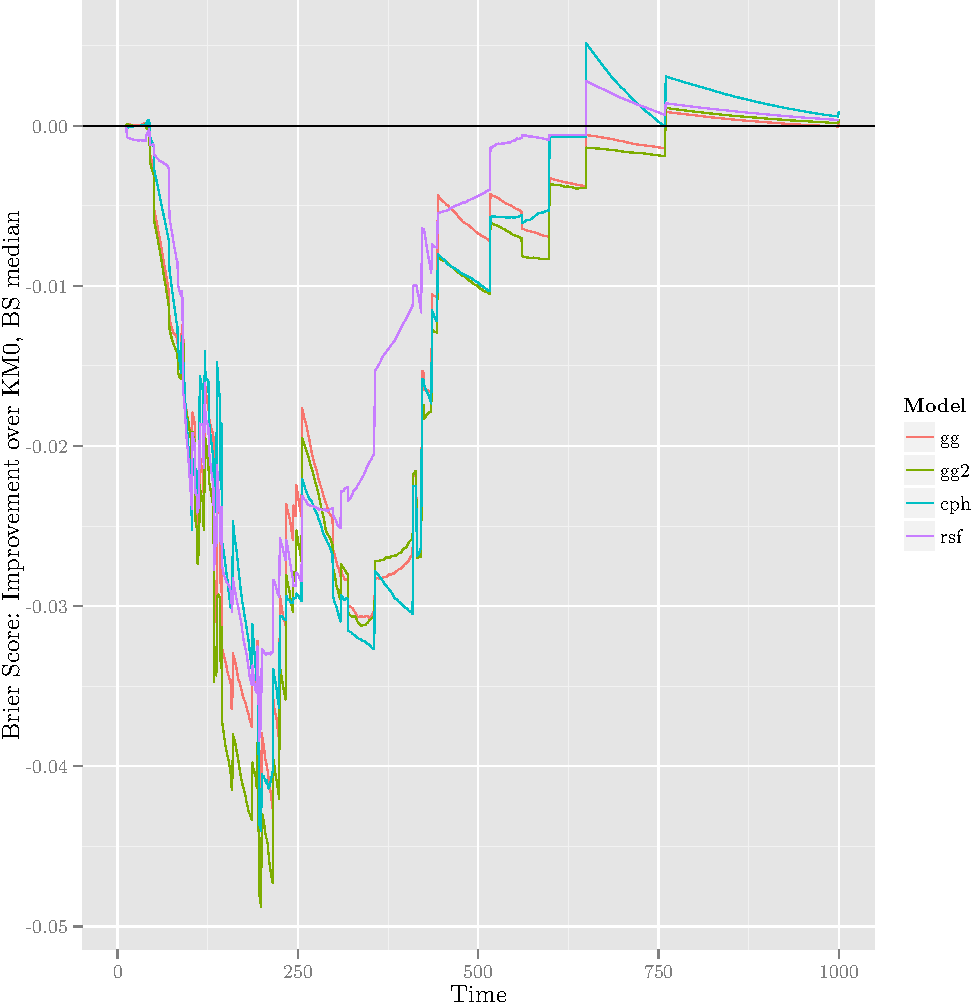
\includegraphics[width=\maxwidth]{figure/05-model-selection-bs-paths-5} 

}


\begin{kframe}\begin{alltt}
\hlkwd{ggplot}\hlstd{(temp,} \hlkwd{aes}\hlstd{(}\hlkwc{x} \hlstd{= Time,} \hlkwc{y} \hlstd{= Q50,} \hlkwc{colour} \hlstd{= Model))} \hlopt{+} \hlkwd{geom_line}\hlstd{()} \hlopt{+} \hlkwd{ylab}\hlstd{(}\hlstr{"Brier Score: Improvement over KM0, BS median"}\hlstd{)} \hlopt{+} \hlkwd{xlim}\hlstd{(}\hlnum{0}\hlstd{,} \hlnum{700}\hlstd{)} \hlopt{+} \hlkwd{geom_hline}\hlstd{(}\hlkwc{yintercept} \hlstd{=} \hlnum{0}\hlstd{)}
\end{alltt}


{\ttfamily\noindent\color{warningcolor}{\#\# Warning: Removed 1200 rows containing missing values (geom\_path).}}\end{kframe}

{\centering 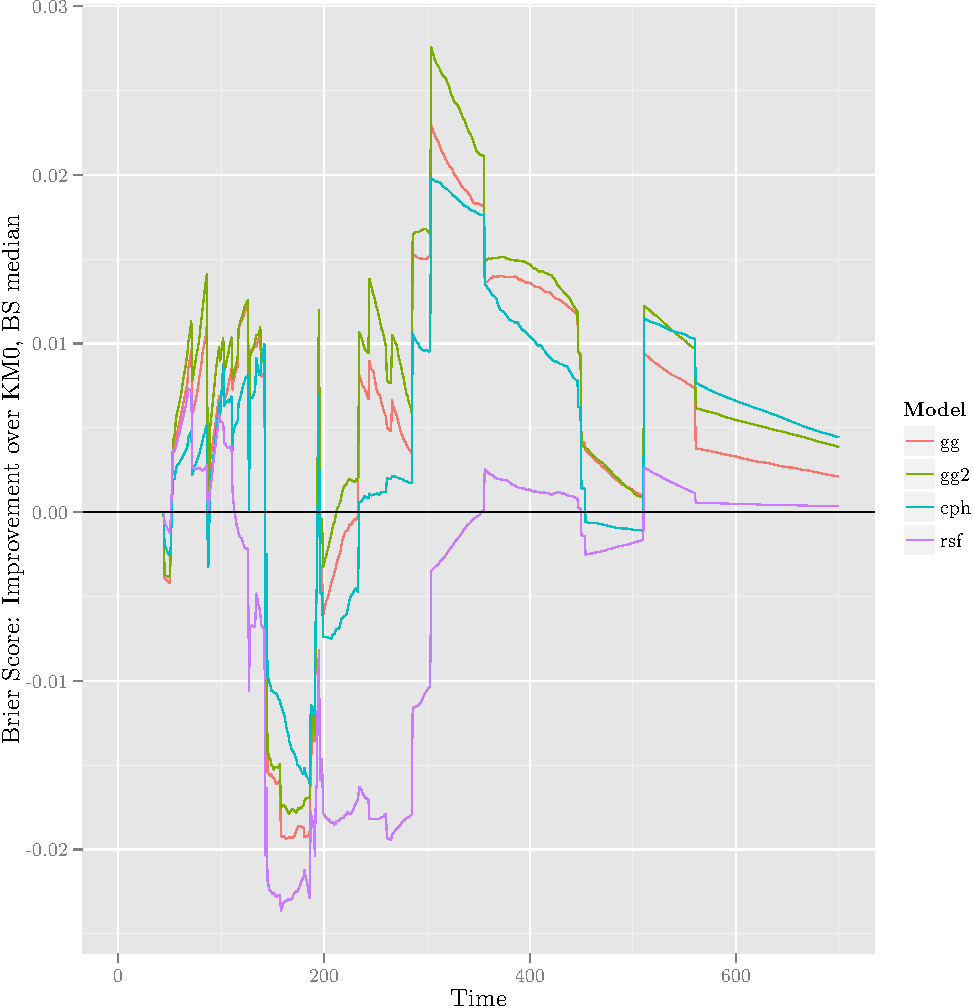
\includegraphics[width=\maxwidth]{figure/05-model-selection-bs-paths-6} 

}



\end{knitrout}

IBS comparisons.
\begin{knitrout}
\definecolor{shadecolor}{rgb}{0.969, 0.969, 0.969}\color{fgcolor}\begin{kframe}
\begin{alltt}
\hlkwd{set.seed}\hlstd{(}\hlnum{20150111}\hlstd{)}
\hlstd{ibsc_boots} \hlkwb{=} \hlkwd{t}\hlstd{(}\hlkwd{sapply}\hlstd{(}\hlnum{1}\hlopt{:}\hlnum{5e2}\hlstd{,} \hlkwa{function}\hlstd{(}\hlkwc{i}\hlstd{) \{}
        \hlkwa{if} \hlstd{(i} \hlopt \hlnum{5e1} \hlopt{==} \hlnum{0}\hlstd{)      \{} \hlkwd{message}\hlstd{(i) \}}
        \hlstd{boot_samp} \hlkwb{=} \hlkwd{sample.int}\hlstd{(}\hlkwd{nrow}\hlstd{(data.val),} \hlkwc{replace} \hlstd{=} \hlnum{TRUE}\hlstd{)}
        \hlstd{gg} \hlkwb{=} \hlkwd{calcIBS}\hlstd{(}\hlkwd{Surv}\hlstd{(data.val}\hlopt{$}\hlstd{Time, data.val}\hlopt{$}\hlstd{DSD)[boot_samp,], ibs_preds_gg[boot_samp,], ibs_times,} \hlkwd{max}\hlstd{(data.val}\hlopt{$}\hlstd{Time[boot_samp]))}\hlopt{$}\hlstd{ibs}
        \hlstd{gg2} \hlkwb{=} \hlkwd{calcIBS}\hlstd{(}\hlkwd{Surv}\hlstd{(data.val}\hlopt{$}\hlstd{Time, data.val}\hlopt{$}\hlstd{DSD)[boot_samp,], ibs_preds_gg2[boot_samp,], ibs_times,} \hlkwd{max}\hlstd{(data.val}\hlopt{$}\hlstd{Time[boot_samp]))}\hlopt{$}\hlstd{ibs}
        \hlstd{cph} \hlkwb{=} \hlkwd{calcIBS}\hlstd{(}\hlkwd{Surv}\hlstd{(data.val}\hlopt{$}\hlstd{Time, data.val}\hlopt{$}\hlstd{DSD)[boot_samp,], ibs_preds_cph[boot_samp,], ibs_times,} \hlkwd{max}\hlstd{(data.val}\hlopt{$}\hlstd{Time[boot_samp]))}\hlopt{$}\hlstd{ibs}
        \hlstd{rsf} \hlkwb{=} \hlkwd{calcIBS}\hlstd{(}\hlkwd{Surv}\hlstd{(data.val}\hlopt{$}\hlstd{Time, data.val}\hlopt{$}\hlstd{DSD)[boot_samp,], ibs_preds_rsf[boot_samp,], ibs_times,} \hlkwd{max}\hlstd{(data.val}\hlopt{$}\hlstd{Time[boot_samp]))}\hlopt{$}\hlstd{ibs}
        \hlstd{km0} \hlkwb{=} \hlkwd{calcIBS}\hlstd{(}\hlkwd{Surv}\hlstd{(data.val}\hlopt{$}\hlstd{Time, data.val}\hlopt{$}\hlstd{DSD)[boot_samp,], ibs_preds_km0[boot_samp,], ibs_times,} \hlkwd{max}\hlstd{(data.val}\hlopt{$}\hlstd{Time[boot_samp]))}\hlopt{$}\hlstd{ibs}
        \hlkwd{c}\hlstd{(gg, gg2, cph, rsf, km0)}
\hlstd{\}))}
\end{alltt}


{\ttfamily\noindent\itshape\color{messagecolor}{\#\# 50\\\#\# 100\\\#\# 150\\\#\# 200\\\#\# 250\\\#\# 300\\\#\# 350\\\#\# 400\\\#\# 450\\\#\# 500}}\begin{alltt}
\hlkwd{colnames}\hlstd{(ibsc_boots)} \hlkwb{=} \hlkwd{c}\hlstd{(}\hlstr{"gg"}\hlstd{,} \hlstr{"gg2"}\hlstd{,} \hlstr{"cph"}\hlstd{,} \hlstr{"rsf"}\hlstd{,} \hlstr{"km0"}\hlstd{)}
\end{alltt}
\end{kframe}
\end{knitrout}

\begin{knitrout}
\definecolor{shadecolor}{rgb}{0.969, 0.969, 0.969}\color{fgcolor}\begin{kframe}
\begin{alltt}
\hlkwd{calcIBS}\hlstd{(}\hlkwd{Surv}\hlstd{(data.val}\hlopt{$}\hlstd{Time, data.val}\hlopt{$}\hlstd{DSD), ibs_preds_gg, ibs_times,} \hlkwd{max}\hlstd{(data.val}\hlopt{$}\hlstd{Time))}\hlopt{$}\hlstd{ibs}
\end{alltt}
\begin{verbatim}
## [1] 147.4
\end{verbatim}
\begin{alltt}
\hlkwd{calcIBS}\hlstd{(}\hlkwd{Surv}\hlstd{(data.val}\hlopt{$}\hlstd{Time, data.val}\hlopt{$}\hlstd{DSD), ibs_preds_gg2, ibs_times,} \hlkwd{max}\hlstd{(data.val}\hlopt{$}\hlstd{Time))}\hlopt{$}\hlstd{ibs}
\end{alltt}
\begin{verbatim}
## [1] 145.6
\end{verbatim}
\begin{alltt}
\hlkwd{calcIBS}\hlstd{(}\hlkwd{Surv}\hlstd{(data.val}\hlopt{$}\hlstd{Time, data.val}\hlopt{$}\hlstd{DSD), ibs_preds_cph, ibs_times,} \hlkwd{max}\hlstd{(data.val}\hlopt{$}\hlstd{Time))}\hlopt{$}\hlstd{ibs}
\end{alltt}
\begin{verbatim}
## [1] 148.6
\end{verbatim}
\begin{alltt}
\hlkwd{calcIBS}\hlstd{(}\hlkwd{Surv}\hlstd{(data.val}\hlopt{$}\hlstd{Time, data.val}\hlopt{$}\hlstd{DSD), ibs_preds_rsf, ibs_times,} \hlkwd{max}\hlstd{(data.val}\hlopt{$}\hlstd{Time))}\hlopt{$}\hlstd{ibs}
\end{alltt}
\begin{verbatim}
## [1] 153.3
\end{verbatim}
\begin{alltt}
\hlkwd{calcIBS}\hlstd{(}\hlkwd{Surv}\hlstd{(data.val}\hlopt{$}\hlstd{Time, data.val}\hlopt{$}\hlstd{DSD), ibs_preds_km0, ibs_times,} \hlkwd{max}\hlstd{(data.val}\hlopt{$}\hlstd{Time))}\hlopt{$}\hlstd{ibs}
\end{alltt}
\begin{verbatim}
## [1] 165.4
\end{verbatim}
\begin{alltt}
\hlkwd{boxplot}\hlstd{(ibsc_boots,} \hlkwc{main} \hlstd{=} \hlstr{"IBS BS Distribution"}\hlstd{,} \hlkwc{ylab} \hlstd{=} \hlstr{"IBS"}\hlstd{)}
\end{alltt}
\end{kframe}

{\centering 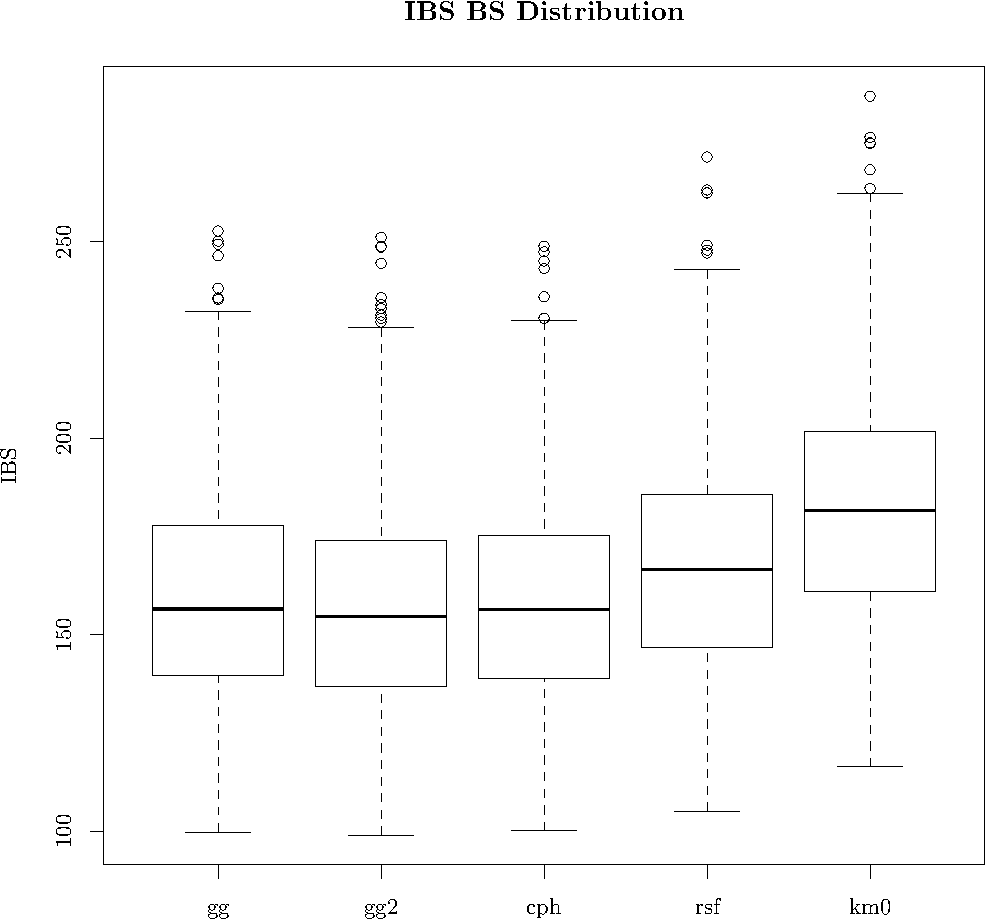
\includegraphics[width=\maxwidth]{figure/05-model-selection-ibs-1} 

}


\begin{kframe}\begin{alltt}
\hlkwd{plot}\hlstd{(}\hlkwd{density}\hlstd{(ibsc_boots[,}\hlnum{1}\hlstd{]),} \hlkwc{col} \hlstd{=} \hlstr{"blue"}\hlstd{,} \hlkwc{lwd} \hlstd{=} \hlnum{2}\hlstd{,} \hlkwc{main} \hlstd{=} \hlstr{"IBS BS Distribution"}\hlstd{,} \hlkwc{xlab} \hlstd{=} \hlstr{"IBS"}\hlstd{)}
\hlkwd{lines}\hlstd{(}\hlkwd{density}\hlstd{(ibsc_boots[,}\hlnum{2}\hlstd{]),} \hlkwc{col} \hlstd{=} \hlstr{"red"}\hlstd{,} \hlkwc{lwd} \hlstd{=} \hlnum{2}\hlstd{)}
\hlkwd{lines}\hlstd{(}\hlkwd{density}\hlstd{(ibsc_boots[,}\hlnum{3}\hlstd{]),} \hlkwc{col} \hlstd{=} \hlstr{"green"}\hlstd{,} \hlkwc{lwd} \hlstd{=} \hlnum{2}\hlstd{)}
\hlkwd{lines}\hlstd{(}\hlkwd{density}\hlstd{(ibsc_boots[,}\hlnum{4}\hlstd{]),} \hlkwc{col} \hlstd{=} \hlstr{"purple"}\hlstd{,} \hlkwc{lwd} \hlstd{=} \hlnum{2}\hlstd{)}
\hlkwd{lines}\hlstd{(}\hlkwd{density}\hlstd{(ibsc_boots[,}\hlnum{5}\hlstd{]),} \hlkwc{col} \hlstd{=} \hlstr{"black"}\hlstd{,} \hlkwc{lwd} \hlstd{=} \hlnum{2}\hlstd{)}
\hlkwd{abline}\hlstd{(}\hlkwc{v} \hlstd{=} \hlkwd{calcIBS}\hlstd{(}\hlkwd{Surv}\hlstd{(data.val}\hlopt{$}\hlstd{Time, data.val}\hlopt{$}\hlstd{DSD), ibs_preds_gg, ibs_times,} \hlkwd{max}\hlstd{(data.val}\hlopt{$}\hlstd{Time))}\hlopt{$}\hlstd{ibs,} \hlkwc{col} \hlstd{=} \hlstr{"blue"}\hlstd{,} \hlkwc{lwd} \hlstd{=} \hlnum{1}\hlstd{)}
\hlkwd{abline}\hlstd{(}\hlkwc{v} \hlstd{=} \hlkwd{calcIBS}\hlstd{(}\hlkwd{Surv}\hlstd{(data.val}\hlopt{$}\hlstd{Time, data.val}\hlopt{$}\hlstd{DSD), ibs_preds_gg2, ibs_times,} \hlkwd{max}\hlstd{(data.val}\hlopt{$}\hlstd{Time))}\hlopt{$}\hlstd{ibs,} \hlkwc{col} \hlstd{=} \hlstr{"red"}\hlstd{,} \hlkwc{lwd} \hlstd{=} \hlnum{1}\hlstd{)}
\hlkwd{abline}\hlstd{(}\hlkwc{v} \hlstd{=} \hlkwd{calcIBS}\hlstd{(}\hlkwd{Surv}\hlstd{(data.val}\hlopt{$}\hlstd{Time, data.val}\hlopt{$}\hlstd{DSD), ibs_preds_cph, ibs_times,} \hlkwd{max}\hlstd{(data.val}\hlopt{$}\hlstd{Time))}\hlopt{$}\hlstd{ibs,} \hlkwc{col} \hlstd{=} \hlstr{"green"}\hlstd{,} \hlkwc{lwd} \hlstd{=} \hlnum{1}\hlstd{)}
\hlkwd{abline}\hlstd{(}\hlkwc{v} \hlstd{=} \hlkwd{calcIBS}\hlstd{(}\hlkwd{Surv}\hlstd{(data.val}\hlopt{$}\hlstd{Time, data.val}\hlopt{$}\hlstd{DSD), ibs_preds_rsf, ibs_times,} \hlkwd{max}\hlstd{(data.val}\hlopt{$}\hlstd{Time))}\hlopt{$}\hlstd{ibs,} \hlkwc{col} \hlstd{=} \hlstr{"purple"}\hlstd{,} \hlkwc{lwd} \hlstd{=} \hlnum{1}\hlstd{)}
\hlkwd{abline}\hlstd{(}\hlkwc{v} \hlstd{=} \hlkwd{calcIBS}\hlstd{(}\hlkwd{Surv}\hlstd{(data.val}\hlopt{$}\hlstd{Time, data.val}\hlopt{$}\hlstd{DSD), ibs_preds_km0, ibs_times,} \hlkwd{max}\hlstd{(data.val}\hlopt{$}\hlstd{Time))}\hlopt{$}\hlstd{ibs,} \hlkwc{col} \hlstd{=} \hlstr{"black"}\hlstd{,} \hlkwc{lwd} \hlstd{=} \hlnum{1}\hlstd{)}
\hlkwd{legend}\hlstd{(}\hlstr{"topright"}\hlstd{,} \hlkwc{legend} \hlstd{=} \hlkwd{c}\hlstd{(}\hlstr{"gg"}\hlstd{,} \hlstr{"gg2"}\hlstd{,} \hlstr{"cph"}\hlstd{,} \hlstr{"rsf"}\hlstd{,} \hlstr{"km0"}\hlstd{),} \hlkwc{col} \hlstd{=} \hlkwd{c}\hlstd{(}\hlstr{"blue"}\hlstd{,} \hlstr{"red"}\hlstd{,} \hlstr{"green"}\hlstd{,} \hlstr{"purple"}\hlstd{,} \hlstr{"black"}\hlstd{),} \hlkwc{lty} \hlstd{=} \hlstr{"solid"}\hlstd{,} \hlkwc{inset} \hlstd{=} \hlnum{0.05}\hlstd{)}
\end{alltt}
\end{kframe}

{\centering 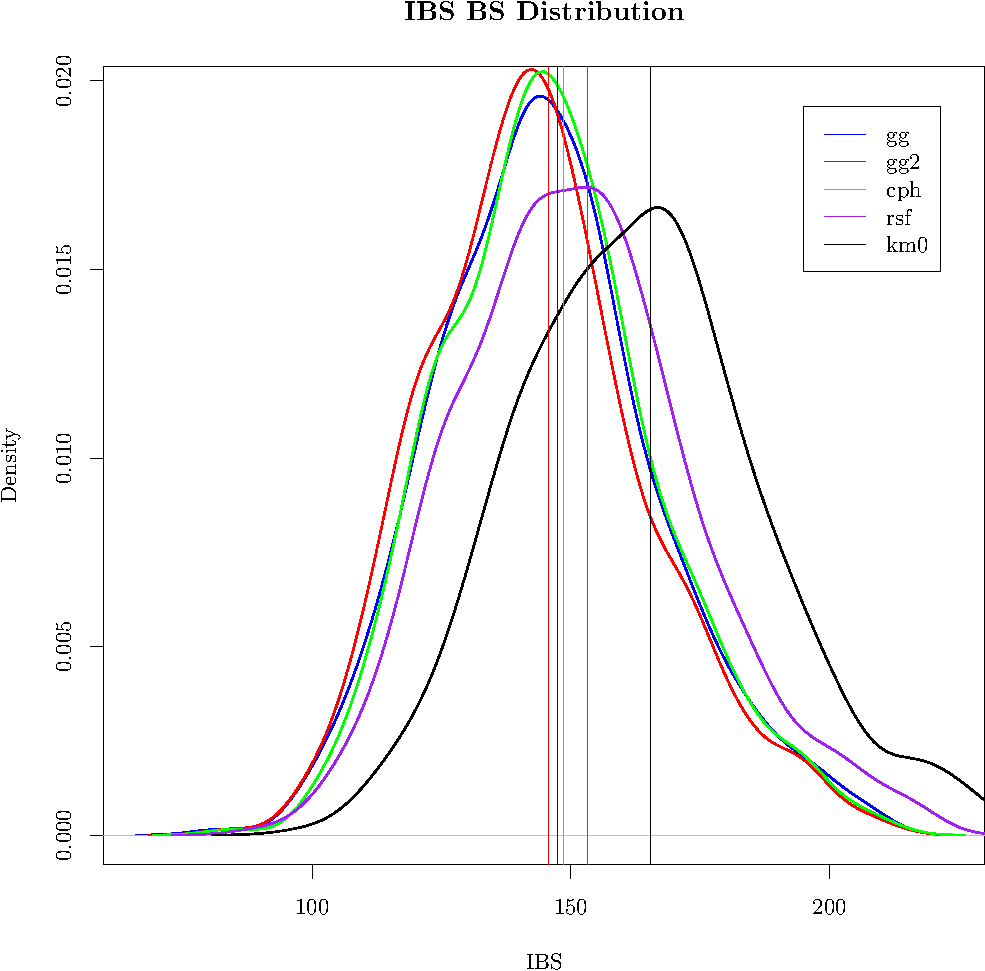
\includegraphics[width=\maxwidth]{figure/05-model-selection-ibs-2} 

}


\begin{kframe}\begin{alltt}
\hlkwd{plot}\hlstd{(}\hlkwd{density}\hlstd{(ibsc_boots[,}\hlnum{5}\hlstd{]} \hlopt{-} \hlstd{ibsc_boots[,}\hlnum{1}\hlstd{]),} \hlkwc{col} \hlstd{=} \hlstr{"blue"}\hlstd{,} \hlkwc{lwd} \hlstd{=} \hlnum{2}\hlstd{,} \hlkwc{main} \hlstd{=} \hlstr{"IBS\textbackslash{}\textbackslash{}_KM0 - IBS\textbackslash{}\textbackslash{}_x BS Distribution"}\hlstd{,} \hlkwc{xlab} \hlstd{=} \hlstr{"IBS"}\hlstd{,} \hlkwc{ylim} \hlstd{=} \hlkwd{c}\hlstd{(}\hlnum{0}\hlstd{,} \hlnum{0.1}\hlstd{))}
\hlkwd{lines}\hlstd{(}\hlkwd{density}\hlstd{(ibsc_boots[,}\hlnum{5}\hlstd{]} \hlopt{-} \hlstd{ibsc_boots[,}\hlnum{2}\hlstd{]),} \hlkwc{col} \hlstd{=} \hlstr{"red"}\hlstd{,} \hlkwc{lwd} \hlstd{=} \hlnum{2}\hlstd{)}
\hlkwd{lines}\hlstd{(}\hlkwd{density}\hlstd{(ibsc_boots[,}\hlnum{5}\hlstd{]} \hlopt{-} \hlstd{ibsc_boots[,}\hlnum{3}\hlstd{]),} \hlkwc{col} \hlstd{=} \hlstr{"green"}\hlstd{,} \hlkwc{lwd} \hlstd{=} \hlnum{2}\hlstd{)}
\hlkwd{lines}\hlstd{(}\hlkwd{density}\hlstd{(ibsc_boots[,}\hlnum{5}\hlstd{]} \hlopt{-} \hlstd{ibsc_boots[,}\hlnum{4}\hlstd{]),} \hlkwc{col} \hlstd{=} \hlstr{"purple"}\hlstd{,} \hlkwc{lwd} \hlstd{=} \hlnum{2}\hlstd{)}
\hlkwd{abline}\hlstd{(}\hlkwc{v} \hlstd{= (}\hlkwd{calcIBS}\hlstd{(}\hlkwd{Surv}\hlstd{(data.val}\hlopt{$}\hlstd{Time, data.val}\hlopt{$}\hlstd{DSD), ibs_preds_km0, ibs_times,} \hlkwd{max}\hlstd{(data.val}\hlopt{$}\hlstd{Time))}\hlopt{$}\hlstd{ibs} \hlopt{-} \hlkwd{calcIBS}\hlstd{(}\hlkwd{Surv}\hlstd{(data.val}\hlopt{$}\hlstd{Time, data.val}\hlopt{$}\hlstd{DSD), ibs_preds_gg, ibs_times,} \hlkwd{max}\hlstd{(data.val}\hlopt{$}\hlstd{Time))}\hlopt{$}\hlstd{ibs),} \hlkwc{col} \hlstd{=} \hlstr{"blue"}\hlstd{,} \hlkwc{lwd} \hlstd{=} \hlnum{1}\hlstd{)}
\hlkwd{abline}\hlstd{(}\hlkwc{v} \hlstd{= (}\hlkwd{calcIBS}\hlstd{(}\hlkwd{Surv}\hlstd{(data.val}\hlopt{$}\hlstd{Time, data.val}\hlopt{$}\hlstd{DSD), ibs_preds_km0, ibs_times,} \hlkwd{max}\hlstd{(data.val}\hlopt{$}\hlstd{Time))}\hlopt{$}\hlstd{ibs} \hlopt{-} \hlkwd{calcIBS}\hlstd{(}\hlkwd{Surv}\hlstd{(data.val}\hlopt{$}\hlstd{Time, data.val}\hlopt{$}\hlstd{DSD), ibs_preds_gg2, ibs_times,} \hlkwd{max}\hlstd{(data.val}\hlopt{$}\hlstd{Time))}\hlopt{$}\hlstd{ibs),} \hlkwc{col} \hlstd{=} \hlstr{"red"}\hlstd{,} \hlkwc{lwd} \hlstd{=} \hlnum{1}\hlstd{)}
\hlkwd{abline}\hlstd{(}\hlkwc{v} \hlstd{= (}\hlkwd{calcIBS}\hlstd{(}\hlkwd{Surv}\hlstd{(data.val}\hlopt{$}\hlstd{Time, data.val}\hlopt{$}\hlstd{DSD), ibs_preds_km0, ibs_times,} \hlkwd{max}\hlstd{(data.val}\hlopt{$}\hlstd{Time))}\hlopt{$}\hlstd{ibs} \hlopt{-} \hlkwd{calcIBS}\hlstd{(}\hlkwd{Surv}\hlstd{(data.val}\hlopt{$}\hlstd{Time, data.val}\hlopt{$}\hlstd{DSD), ibs_preds_cph, ibs_times,} \hlkwd{max}\hlstd{(data.val}\hlopt{$}\hlstd{Time))}\hlopt{$}\hlstd{ibs),} \hlkwc{col} \hlstd{=} \hlstr{"green"}\hlstd{,} \hlkwc{lwd} \hlstd{=} \hlnum{1}\hlstd{)}
\hlkwd{abline}\hlstd{(}\hlkwc{v} \hlstd{= (}\hlkwd{calcIBS}\hlstd{(}\hlkwd{Surv}\hlstd{(data.val}\hlopt{$}\hlstd{Time, data.val}\hlopt{$}\hlstd{DSD), ibs_preds_km0, ibs_times,} \hlkwd{max}\hlstd{(data.val}\hlopt{$}\hlstd{Time))}\hlopt{$}\hlstd{ibs} \hlopt{-} \hlkwd{calcIBS}\hlstd{(}\hlkwd{Surv}\hlstd{(data.val}\hlopt{$}\hlstd{Time, data.val}\hlopt{$}\hlstd{DSD), ibs_preds_rsf, ibs_times,} \hlkwd{max}\hlstd{(data.val}\hlopt{$}\hlstd{Time))}\hlopt{$}\hlstd{ibs),} \hlkwc{col} \hlstd{=} \hlstr{"purple"}\hlstd{,} \hlkwc{lwd} \hlstd{=} \hlnum{1}\hlstd{)}
\hlkwd{legend}\hlstd{(}\hlstr{"topright"}\hlstd{,} \hlkwc{legend} \hlstd{=} \hlkwd{c}\hlstd{(}\hlstr{"gg"}\hlstd{,} \hlstr{"gg2"}\hlstd{,} \hlstr{"cph"}\hlstd{,} \hlstr{"rsf"}\hlstd{),} \hlkwc{col} \hlstd{=} \hlkwd{c}\hlstd{(}\hlstr{"blue"}\hlstd{,} \hlstr{"red"}\hlstd{,} \hlstr{"green"}\hlstd{,} \hlstr{"purple"}\hlstd{),} \hlkwc{lty} \hlstd{=} \hlstr{"solid"}\hlstd{,} \hlkwc{inset} \hlstd{=} \hlnum{0.05}\hlstd{)}
\end{alltt}
\end{kframe}

{\centering 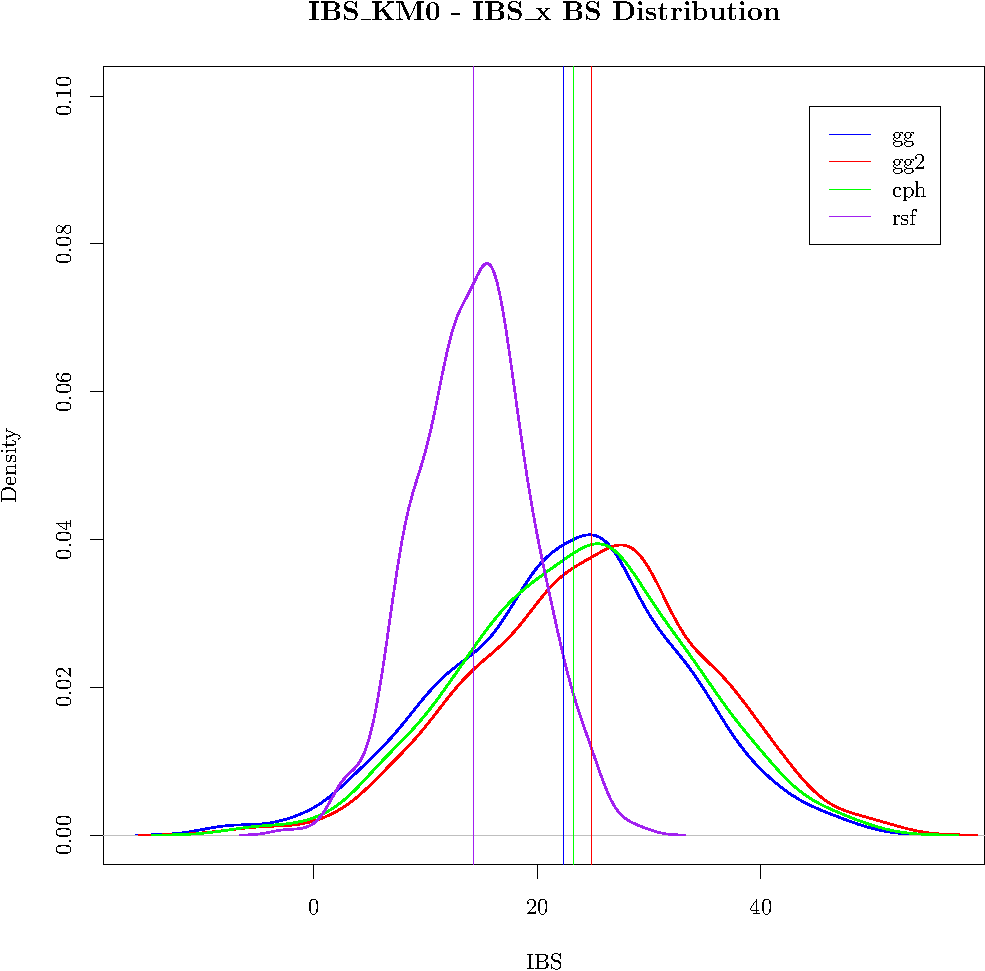
\includegraphics[width=\maxwidth]{figure/05-model-selection-ibs-3} 

}



\end{knitrout}

Do some proper BCA bootstrapping on the differences, just as a double-check test.
\begin{knitrout}
\definecolor{shadecolor}{rgb}{0.969, 0.969, 0.969}\color{fgcolor}\begin{kframe}
\begin{alltt}
\hlkwd{set.seed}\hlstd{(}\hlnum{20150111}\hlstd{)}
\hlstd{ibsc_boots2} \hlkwb{=} \hlkwd{boot}\hlstd{(data.val,} \hlkwc{statistic} \hlstd{=} \hlkwa{function}\hlstd{(}\hlkwc{d}\hlstd{,} \hlkwc{i}\hlstd{) \{}
        \hlstd{gg} \hlkwb{=} \hlkwd{calcIBS}\hlstd{(}\hlkwd{Surv}\hlstd{(d}\hlopt{$}\hlstd{Time, d}\hlopt{$}\hlstd{DSD)[i,], ibs_preds_gg[i,], ibs_times,} \hlkwd{max}\hlstd{(d}\hlopt{$}\hlstd{Time[i]))}\hlopt{$}\hlstd{ibs}
        \hlstd{gg2} \hlkwb{=} \hlkwd{calcIBS}\hlstd{(}\hlkwd{Surv}\hlstd{(d}\hlopt{$}\hlstd{Time, d}\hlopt{$}\hlstd{DSD)[i,], ibs_preds_gg2[i,], ibs_times,} \hlkwd{max}\hlstd{(d}\hlopt{$}\hlstd{Time[i]))}\hlopt{$}\hlstd{ibs}
        \hlstd{cph} \hlkwb{=} \hlkwd{calcIBS}\hlstd{(}\hlkwd{Surv}\hlstd{(d}\hlopt{$}\hlstd{Time, d}\hlopt{$}\hlstd{DSD)[i,], ibs_preds_cph[i,], ibs_times,} \hlkwd{max}\hlstd{(d}\hlopt{$}\hlstd{Time[i]))}\hlopt{$}\hlstd{ibs}
        \hlstd{rsf} \hlkwb{=} \hlkwd{calcIBS}\hlstd{(}\hlkwd{Surv}\hlstd{(d}\hlopt{$}\hlstd{Time, d}\hlopt{$}\hlstd{DSD)[i,], ibs_preds_rsf[i,], ibs_times,} \hlkwd{max}\hlstd{(d}\hlopt{$}\hlstd{Time[i]))}\hlopt{$}\hlstd{ibs}
        \hlstd{km0} \hlkwb{=} \hlkwd{calcIBS}\hlstd{(}\hlkwd{Surv}\hlstd{(d}\hlopt{$}\hlstd{Time, d}\hlopt{$}\hlstd{DSD)[i,], ibs_preds_km0[i,], ibs_times,} \hlkwd{max}\hlstd{(d}\hlopt{$}\hlstd{Time[i]))}\hlopt{$}\hlstd{ibs}
        \hlkwd{c}\hlstd{(gg} \hlopt{-} \hlstd{km0, gg2} \hlopt{-} \hlstd{km0, cph} \hlopt{-} \hlstd{km0, rsf} \hlopt{-} \hlstd{km0, gg} \hlopt{-} \hlstd{rsf, gg2} \hlopt{-} \hlstd{rsf, cph} \hlopt{-} \hlstd{rsf, gg} \hlopt{-} \hlstd{cph, gg2} \hlopt{-} \hlstd{cph, gg} \hlopt{-} \hlstd{gg2)}
\hlstd{\},} \hlkwc{R} \hlstd{=} \hlnum{500}\hlstd{)}
\hlstd{ibsc_boots2_ci} \hlkwb{=} \hlkwd{t}\hlstd{(}\hlkwd{sapply}\hlstd{(}\hlnum{1}\hlopt{:}\hlkwd{length}\hlstd{(ibsc_boots2}\hlopt{$}\hlstd{t0),} \hlkwa{function}\hlstd{(}\hlkwc{i}\hlstd{)} \hlkwd{boot.ci}\hlstd{(ibsc_boots2,} \hlkwc{index} \hlstd{= i,} \hlkwc{type} \hlstd{=} \hlstr{"bca"}\hlstd{)}\hlopt{$}\hlstd{bca))}
\hlkwd{rownames}\hlstd{(ibsc_boots2_ci)} \hlkwb{=} \hlkwd{c}\hlstd{(}\hlstr{"gg-km0"}\hlstd{,} \hlstr{"gg2-km0"}\hlstd{,} \hlstr{"cph-km0"}\hlstd{,} \hlstr{"rsf-km0"}\hlstd{,} \hlstr{"gg-rsf"}\hlstd{,} \hlstr{"gg2-rsf"}\hlstd{,} \hlstr{"cph-rsf"}\hlstd{,} \hlstr{"gg-cph"}\hlstd{,} \hlstr{"gg2-cph"}\hlstd{,} \hlstr{"gg-gg2"}\hlstd{)}
\hlkwd{colnames}\hlstd{(ibsc_boots2_ci)} \hlkwb{=} \hlkwd{c}\hlstd{(}\hlstr{"level"}\hlstd{,} \hlstr{"orderi1"}\hlstd{,} \hlstr{"orderi2"}\hlstd{,} \hlstr{"lci"}\hlstd{,} \hlstr{"uci"}\hlstd{)}
\hlstd{ibsc_boots2}
\end{alltt}
\begin{verbatim}
## 
## ORDINARY NONPARAMETRIC BOOTSTRAP
## 
## 
## Call:
## boot(data = data.val, statistic = function(d, i) {
##     gg = calcIBS(Surv(d$Time, d$DSD)[i, ], ibs_preds_gg[i, ], 
##         ibs_times, max(d$Time[i]))$ibs
##     gg2 = calcIBS(Surv(d$Time, d$DSD)[i, ], ibs_preds_gg2[i, 
##         ], ibs_times, max(d$Time[i]))$ibs
##     cph = calcIBS(Surv(d$Time, d$DSD)[i, ], ibs_preds_cph[i, 
##         ], ibs_times, max(d$Time[i]))$ibs
##     rsf = calcIBS(Surv(d$Time, d$DSD)[i, ], ibs_preds_rsf[i, 
##         ], ibs_times, max(d$Time[i]))$ibs
##     km0 = calcIBS(Surv(d$Time, d$DSD)[i, ], ibs_preds_km0[i, 
##         ], ibs_times, max(d$Time[i]))$ibs
##     c(gg - km0, gg2 - km0, cph - km0, rsf - km0, gg - rsf, gg2 - 
##         rsf, cph - rsf, gg - cph, gg2 - cph, gg - gg2)
## }, R = 500)
## 
## 
## Bootstrap Statistics :
##      original   bias    std. error
## t1*   -17.960  0.16202       9.092
## t2*   -19.764  0.08589       9.303
## t3*   -16.830 -0.34992       9.293
## t4*   -12.092  0.06313       4.847
## t5*    -5.868  0.09888       4.847
## t6*    -7.672  0.02275       5.138
## t7*    -4.738 -0.41305       5.075
## t8*    -1.129  0.51193       2.188
## t9*    -2.934  0.43580       1.239
## t10*    1.805  0.07613       2.012
\end{verbatim}
\begin{alltt}
\hlstd{ibsc_boots2_ci}
\end{alltt}
\begin{verbatim}
##         level orderi1 orderi2     lci      uci
## gg-km0   0.95   12.62   488.6 -36.586  0.04987
## gg2-km0  0.95   13.26   489.1 -38.095 -0.93649
## cph-km0  0.95   15.77   490.9 -35.135  1.22396
## rsf-km0  0.95   15.92   491.0 -21.344 -1.94556
## gg-rsf   0.95   16.84   491.8 -13.848  4.78985
## gg2-rsf  0.95   13.27   489.1 -17.593  2.48774
## cph-rsf  0.95   16.67   491.4 -14.727  4.96039
## gg-cph   0.95    6.57   477.5  -5.556  3.09545
## gg2-cph  0.95    1.63   442.8  -5.680 -1.02330
## gg-gg2   0.95   13.43   489.4  -2.239  5.99125
\end{verbatim}
\end{kframe}
\end{knitrout}
All models perform equivalently on the validation set.  Select the simplest: gg.


%%%%%%%%%%%%%%%%%%%%%%%%%%%%%%%%%%%%%%%%%%%%%%%%%%%%%%%%%%%%%%%%%%%%%%
% CALCULATE AND SAVE FINAL MODEL
%%%%%%%%%%%%%%%%%%%%%%%%%%%%%%%%%%%%%%%%%%%%%%%%%%%%%%%%%%%%%%%%%%%%%%
Final model fitting:
\begin{knitrout}
\definecolor{shadecolor}{rgb}{0.969, 0.969, 0.969}\color{fgcolor}\begin{kframe}
\begin{alltt}
\hlstd{data.all} \hlkwb{=} \hlkwd{rbind}\hlstd{(data[}\hlkwd{colnames}\hlstd{(data.val)], data.val)}
\hlkwd{head}\hlstd{(data.all)}
\end{alltt}
\begin{verbatim}
##           Time  DSD  SexM AgeCent LocBody SizeCent    A2    A4
## NSWPCN_4   937 TRUE  TRUE     -16   FALSE       -1 FALSE  TRUE
## NSWPCN_7   247 TRUE FALSE      -1   FALSE       -2 FALSE  TRUE
## NSWPCN_10  177 TRUE  TRUE      -9   FALSE       10 FALSE  TRUE
## NSWPCN_13  247 TRUE FALSE     -19    TRUE       20 FALSE  TRUE
## NSWPCN_20  256 TRUE FALSE      -8   FALSE        0 FALSE  TRUE
## NSWPCN_21  763 TRUE FALSE      -1   FALSE       -2 FALSE FALSE
\end{verbatim}
\begin{alltt}
\hlstd{fit.final.gg} \hlkwb{=} \hlkwd{flexsurvreg}\hlstd{(}\hlkwd{Surv}\hlstd{(Time, DSD)} \hlopt{~} \hlstd{SexM} \hlopt{+} \hlstd{SizeCent} \hlopt{+} \hlstd{A2} \hlopt{+} \hlstd{A4,}
        \hlkwc{anc} \hlstd{=} \hlkwd{list}\hlstd{(}
                \hlkwc{sigma} \hlstd{=} \hlopt{~} \hlstd{SexM,}
                \hlkwc{Q} \hlstd{=} \hlopt{~} \hlstd{SexM),}
        \hlkwc{data} \hlstd{= data.all,} \hlkwc{dist} \hlstd{=} \hlstr{"gengamma"}\hlstd{)}
\hlstd{fit.final.gg2} \hlkwb{=} \hlkwd{flexsurvreg}\hlstd{(}\hlkwd{Surv}\hlstd{(Time, DSD)} \hlopt{~} \hlstd{SexM} \hlopt{+} \hlstd{SizeCent} \hlopt{+} \hlstd{A2} \hlopt{+} \hlstd{A4} \hlopt{+} \hlkwd{I}\hlstd{(SexM} \hlopt{==} \hlnum{FALSE} \hlopt{&} \hlstd{A2} \hlopt{==} \hlnum{FALSE} \hlopt{&} \hlstd{A4} \hlopt{==} \hlnum{FALSE}\hlstd{),}
    \hlkwc{anc} \hlstd{=} \hlkwd{list}\hlstd{(}
        \hlkwc{sigma} \hlstd{=} \hlopt{~} \hlstd{SexM,}
        \hlkwc{Q} \hlstd{=} \hlopt{~} \hlstd{SexM),}
    \hlkwc{data} \hlstd{= data.all,} \hlkwc{dist} \hlstd{=} \hlstr{"gengamma"}\hlstd{)}
\hlstd{fit.final.cph} \hlkwb{=} \hlkwd{coxph}\hlstd{(}\hlkwd{Surv}\hlstd{(Time, DSD)} \hlopt{~} \hlkwd{strata}\hlstd{(SexM)} \hlopt{+} \hlstd{SizeCent} \hlopt{+} \hlstd{A2} \hlopt{+} \hlstd{A4,} \hlkwc{data} \hlstd{= data.all,} \hlkwc{x} \hlstd{=} \hlnum{TRUE}\hlstd{,} \hlkwc{y} \hlstd{=} \hlnum{TRUE}\hlstd{,} \hlkwc{model} \hlstd{=} \hlnum{TRUE}\hlstd{)}
\hlkwd{set.seed}\hlstd{(}\hlnum{20150111}\hlstd{)}
\hlstd{fit.final.rsf} \hlkwb{=} \hlkwd{rfsrc}\hlstd{(}\hlkwd{Surv}\hlstd{(Time, DSD)} \hlopt{~} \hlstd{SexM} \hlopt{+} \hlstd{AgeCent} \hlopt{+} \hlstd{LocBody} \hlopt{+} \hlstd{SizeCent} \hlopt{+} \hlstd{A2} \hlopt{+} \hlstd{A4,} \hlkwc{data} \hlstd{= data.all,} \hlkwc{mtry} \hlstd{=} \hlnum{1}\hlstd{,} \hlkwc{splitrule} \hlstd{=} \hlstr{"logrankscore"}\hlstd{,} \hlkwc{nsplit} \hlstd{=} \hlnum{2}\hlstd{,} \hlkwc{ntree} \hlstd{=} \hlnum{1000}\hlstd{)}
\hlstd{fit.final.km0} \hlkwb{=} \hlkwd{survfit}\hlstd{(}\hlkwd{Surv}\hlstd{(Time, DSD)} \hlopt{~} \hlnum{1}\hlstd{, data.all)}
\hlkwd{saveRDS}\hlstd{(}\hlkwd{list}\hlstd{(}\hlkwc{gg} \hlstd{= fit.final.gg,} \hlkwc{km0} \hlstd{= fit.final.km0,} \hlkwc{gg2} \hlstd{= fit.final.gg2,} \hlkwc{cph} \hlstd{= fit.final.cph,} \hlkwc{rsf} \hlstd{= fit.final.rsf,} \hlkwc{data.train} \hlstd{= data.all),} \hlkwc{file} \hlstd{=} \hlstr{"05_final_model.rds"}\hlstd{)}
\end{alltt}
\end{kframe}
\end{knitrout}

%%%%%%%%%%%%%%%%%%%%%%%%%%%%%%%%%%%%%%%%%%%%%%%%%%%%%%%%%%%%%%%%%%%%%%
% THE END
%%%%%%%%%%%%%%%%%%%%%%%%%%%%%%%%%%%%%%%%%%%%%%%%%%%%%%%%%%%%%%%%%%%%%%
\section{Session information}
\begin{knitrout}
\definecolor{shadecolor}{rgb}{0.969, 0.969, 0.969}\color{fgcolor}\begin{kframe}
\begin{alltt}
\hlkwd{sessionInfo}\hlstd{()}
\end{alltt}
\begin{verbatim}
## R version 3.1.1 (2014-07-10)
## Platform: x86_64-unknown-linux-gnu (64-bit)
## 
## locale:
##  [1] LC_CTYPE=en_US.UTF-8          LC_NUMERIC=C                 
##  [3] LC_TIME=en_US.UTF-8           LC_COLLATE=en_US.UTF-8       
##  [5] LC_MONETARY=en_US.UTF-8       LC_MESSAGES=en_US.UTF-8      
##  [7] LC_PAPER=en_US.UTF-8          LC_NAME=en_US.UTF-8          
##  [9] LC_ADDRESS=en_US.UTF-8        LC_TELEPHONE=en_US.UTF-8     
## [11] LC_MEASUREMENT=en_US.UTF-8    LC_IDENTIFICATION=en_US.UTF-8
## 
## attached base packages:
## [1] parallel  splines   methods   stats     graphics  grDevices utils    
## [8] datasets  base     
## 
## other attached packages:
##  [1] timeROC_0.2           timereg_1.8.6         mvtnorm_1.0-1        
##  [4] pec_2.4.4             boot_1.3-13           MASS_7.3-35          
##  [7] ggplot2_1.0.0         plyr_1.8.1            reshape2_1.4         
## [10] randomForestSRC_1.5.5 flexsurv_0.5          glmulti_1.0.7        
## [13] rJava_0.9-6           survival_2.37-7       tikzDevice_0.7.0     
## [16] filehash_2.2-2        knitr_1.8            
## 
## loaded via a namespace (and not attached):
##  [1] codetools_0.2-9  colorspace_1.2-4 deSolve_1.11     digest_0.6.4    
##  [5] evaluate_0.5.5   foreach_1.4.2    formatR_1.0      grid_3.1.1      
##  [9] gtable_0.1.2     highr_0.4        iterators_1.0.7  labeling_0.3    
## [13] lava_1.3         muhaz_1.2.6      munsell_0.4.2    prodlim_1.5.1   
## [17] proto_0.3-10     Rcpp_0.11.3      scales_0.2.4     stringr_0.6.2   
## [21] tools_3.1.1
\end{verbatim}
\end{kframe}
\end{knitrout}

\end{document}



